% Options for packages loaded elsewhere
\PassOptionsToPackage{unicode}{hyperref}
\PassOptionsToPackage{hyphens}{url}
%
\documentclass[
]{article}
\usepackage{amsmath,amssymb}
\usepackage{lmodern}
\usepackage{iftex}
\ifPDFTeX
  \usepackage[T1]{fontenc}
  \usepackage[utf8]{inputenc}
  \usepackage{textcomp} % provide euro and other symbols
\else % if luatex or xetex
  \usepackage{unicode-math}
  \defaultfontfeatures{Scale=MatchLowercase}
  \defaultfontfeatures[\rmfamily]{Ligatures=TeX,Scale=1}
\fi
% Use upquote if available, for straight quotes in verbatim environments
\IfFileExists{upquote.sty}{\usepackage{upquote}}{}
\IfFileExists{microtype.sty}{% use microtype if available
  \usepackage[]{microtype}
  \UseMicrotypeSet[protrusion]{basicmath} % disable protrusion for tt fonts
}{}
\usepackage{xcolor}
\usepackage[margin=1in]{geometry}
\usepackage{color}
\usepackage{fancyvrb}
\newcommand{\VerbBar}{|}
\newcommand{\VERB}{\Verb[commandchars=\\\{\}]}
\DefineVerbatimEnvironment{Highlighting}{Verbatim}{commandchars=\\\{\}}
% Add ',fontsize=\small' for more characters per line
\usepackage{framed}
\definecolor{shadecolor}{RGB}{248,248,248}
\newenvironment{Shaded}{\begin{snugshade}}{\end{snugshade}}
\newcommand{\AlertTok}[1]{\textcolor[rgb]{0.94,0.16,0.16}{#1}}
\newcommand{\AnnotationTok}[1]{\textcolor[rgb]{0.56,0.35,0.01}{\textbf{\textit{#1}}}}
\newcommand{\AttributeTok}[1]{\textcolor[rgb]{0.77,0.63,0.00}{#1}}
\newcommand{\BaseNTok}[1]{\textcolor[rgb]{0.00,0.00,0.81}{#1}}
\newcommand{\BuiltInTok}[1]{#1}
\newcommand{\CharTok}[1]{\textcolor[rgb]{0.31,0.60,0.02}{#1}}
\newcommand{\CommentTok}[1]{\textcolor[rgb]{0.56,0.35,0.01}{\textit{#1}}}
\newcommand{\CommentVarTok}[1]{\textcolor[rgb]{0.56,0.35,0.01}{\textbf{\textit{#1}}}}
\newcommand{\ConstantTok}[1]{\textcolor[rgb]{0.00,0.00,0.00}{#1}}
\newcommand{\ControlFlowTok}[1]{\textcolor[rgb]{0.13,0.29,0.53}{\textbf{#1}}}
\newcommand{\DataTypeTok}[1]{\textcolor[rgb]{0.13,0.29,0.53}{#1}}
\newcommand{\DecValTok}[1]{\textcolor[rgb]{0.00,0.00,0.81}{#1}}
\newcommand{\DocumentationTok}[1]{\textcolor[rgb]{0.56,0.35,0.01}{\textbf{\textit{#1}}}}
\newcommand{\ErrorTok}[1]{\textcolor[rgb]{0.64,0.00,0.00}{\textbf{#1}}}
\newcommand{\ExtensionTok}[1]{#1}
\newcommand{\FloatTok}[1]{\textcolor[rgb]{0.00,0.00,0.81}{#1}}
\newcommand{\FunctionTok}[1]{\textcolor[rgb]{0.00,0.00,0.00}{#1}}
\newcommand{\ImportTok}[1]{#1}
\newcommand{\InformationTok}[1]{\textcolor[rgb]{0.56,0.35,0.01}{\textbf{\textit{#1}}}}
\newcommand{\KeywordTok}[1]{\textcolor[rgb]{0.13,0.29,0.53}{\textbf{#1}}}
\newcommand{\NormalTok}[1]{#1}
\newcommand{\OperatorTok}[1]{\textcolor[rgb]{0.81,0.36,0.00}{\textbf{#1}}}
\newcommand{\OtherTok}[1]{\textcolor[rgb]{0.56,0.35,0.01}{#1}}
\newcommand{\PreprocessorTok}[1]{\textcolor[rgb]{0.56,0.35,0.01}{\textit{#1}}}
\newcommand{\RegionMarkerTok}[1]{#1}
\newcommand{\SpecialCharTok}[1]{\textcolor[rgb]{0.00,0.00,0.00}{#1}}
\newcommand{\SpecialStringTok}[1]{\textcolor[rgb]{0.31,0.60,0.02}{#1}}
\newcommand{\StringTok}[1]{\textcolor[rgb]{0.31,0.60,0.02}{#1}}
\newcommand{\VariableTok}[1]{\textcolor[rgb]{0.00,0.00,0.00}{#1}}
\newcommand{\VerbatimStringTok}[1]{\textcolor[rgb]{0.31,0.60,0.02}{#1}}
\newcommand{\WarningTok}[1]{\textcolor[rgb]{0.56,0.35,0.01}{\textbf{\textit{#1}}}}
\usepackage{longtable,booktabs,array}
\usepackage{calc} % for calculating minipage widths
% Correct order of tables after \paragraph or \subparagraph
\usepackage{etoolbox}
\makeatletter
\patchcmd\longtable{\par}{\if@noskipsec\mbox{}\fi\par}{}{}
\makeatother
% Allow footnotes in longtable head/foot
\IfFileExists{footnotehyper.sty}{\usepackage{footnotehyper}}{\usepackage{footnote}}
\makesavenoteenv{longtable}
\usepackage{graphicx}
\makeatletter
\def\maxwidth{\ifdim\Gin@nat@width>\linewidth\linewidth\else\Gin@nat@width\fi}
\def\maxheight{\ifdim\Gin@nat@height>\textheight\textheight\else\Gin@nat@height\fi}
\makeatother
% Scale images if necessary, so that they will not overflow the page
% margins by default, and it is still possible to overwrite the defaults
% using explicit options in \includegraphics[width, height, ...]{}
\setkeys{Gin}{width=\maxwidth,height=\maxheight,keepaspectratio}
% Set default figure placement to htbp
\makeatletter
\def\fps@figure{htbp}
\makeatother
\setlength{\emergencystretch}{3em} % prevent overfull lines
\providecommand{\tightlist}{%
  \setlength{\itemsep}{0pt}\setlength{\parskip}{0pt}}
\setcounter{secnumdepth}{5}
\usepackage{float} \floatplacement{figure}{H}
\usepackage{booktabs}
\usepackage{longtable}
\usepackage{array}
\usepackage{multirow}
\usepackage{wrapfig}
\usepackage{float}
\usepackage{colortbl}
\usepackage{pdflscape}
\usepackage{tabu}
\usepackage{threeparttable}
\usepackage{threeparttablex}
\usepackage[normalem]{ulem}
\usepackage{makecell}
\usepackage{xcolor}
\ifLuaTeX
  \usepackage{selnolig}  % disable illegal ligatures
\fi
\IfFileExists{bookmark.sty}{\usepackage{bookmark}}{\usepackage{hyperref}}
\IfFileExists{xurl.sty}{\usepackage{xurl}}{} % add URL line breaks if available
\urlstyle{same} % disable monospaced font for URLs
\hypersetup{
  pdftitle={everyday\_CI},
  pdfauthor={Meg Cychosz},
  hidelinks,
  pdfcreator={LaTeX via pandoc}}

\title{everyday\_CI}
\author{Meg Cychosz}
\date{11 January 2023}

\begin{document}
\maketitle

\begin{Shaded}
\begin{Highlighting}[]
\NormalTok{matches }\OtherTok{\textless{}{-}} \FunctionTok{read.csv}\NormalTok{(}\StringTok{\textquotesingle{}dataframes/CI\_TH\_matches.csv\textquotesingle{}}\NormalTok{) }\SpecialCharTok{\%\textgreater{}\%} 
  \FunctionTok{select}\NormalTok{(}\SpecialCharTok{{-}}\NormalTok{gender)}

\NormalTok{match\_info }\OtherTok{\textless{}{-}}\NormalTok{ matches }\SpecialCharTok{\%\textgreater{}\%} \FunctionTok{select}\NormalTok{(match, child\_id) }
\end{Highlighting}
\end{Shaded}

\begin{Shaded}
\begin{Highlighting}[]
\CommentTok{\# this code is shared for presentation purposes only}
\CommentTok{\# the results are already constructed into csv files}
\CommentTok{\# which are loaded in the following chunk}

\CommentTok{\# get LENA measures}
\NormalTok{pre\_its\_df }\OtherTok{\textless{}{-}}\NormalTok{ plyr}\SpecialCharTok{::}\FunctionTok{ldply}\NormalTok{( }\AttributeTok{.data =} \FunctionTok{list.files}\NormalTok{(}\AttributeTok{pattern=}\StringTok{"*its\_info.csv"}\NormalTok{, }\CommentTok{\# info about recording and child}
                                    \AttributeTok{recursive=}\ConstantTok{TRUE}\NormalTok{),}
                    \AttributeTok{.fun =}\NormalTok{ read.csv,}\AttributeTok{colClasses=}\FunctionTok{c}\NormalTok{(}\StringTok{"child\_id"}\OtherTok{=}\StringTok{"character"}\NormalTok{)) }\SpecialCharTok{\%\textgreater{}\%}
  \FunctionTok{select}\NormalTok{(}\SpecialCharTok{{-}}\NormalTok{X, }\SpecialCharTok{{-}}\NormalTok{DOB) }\SpecialCharTok{\%\textgreater{}\%}
  \FunctionTok{filter}\NormalTok{(child\_id }\SpecialCharTok{\%in\%}\NormalTok{ matches}\SpecialCharTok{$}\NormalTok{child\_id) }\SpecialCharTok{\%\textgreater{}\%}
  \FunctionTok{mutate}\NormalTok{(}\AttributeTok{endTimeSecs=}\FunctionTok{case\_when}\NormalTok{(child\_id}\SpecialCharTok{==}\StringTok{\textquotesingle{}177RTP1\textquotesingle{}} \SpecialCharTok{\textasciitilde{}} \StringTok{"46214.05S"}\NormalTok{,   }\CommentTok{\# three participants paused their recordings briefly }
                              \ConstantTok{TRUE} \SpecialCharTok{\textasciitilde{}} \StringTok{"57599.99S"}\NormalTok{)) }\SpecialCharTok{\%\textgreater{}\%}              \CommentTok{\# only one participant truly had a \textless{}16hr recording}
                             \FunctionTok{mutate}\NormalTok{(}\AttributeTok{corpus =} \FunctionTok{substring}\NormalTok{(child\_id, }\DecValTok{4}\NormalTok{, }\DecValTok{4}\NormalTok{)) }\CommentTok{\# create a variable for corpus  Jessica)}
                                                                    \CommentTok{\# note that endClockTime is wrong here!}
                                                                    \CommentTok{\# which is fine bc I\textquotesingle{}m not currently using it, but may                                                                         eventually}

\NormalTok{R }\OtherTok{\textless{}{-}}\NormalTok{ pre\_its\_df }\SpecialCharTok{\%\textgreater{}\%} 
  \FunctionTok{filter}\NormalTok{(corpus}\SpecialCharTok{==}\StringTok{\textquotesingle{}R\textquotesingle{}} \SpecialCharTok{|}\NormalTok{ corpus }\SpecialCharTok{==} \StringTok{\textquotesingle{}J\textquotesingle{}}\NormalTok{) }\SpecialCharTok{\%\textgreater{}\%} \CommentTok{\# timezone reported in GMT so we convert to EST and CST here }
  \FunctionTok{mutate}\NormalTok{(}\AttributeTok{startTimestamp =} \FunctionTok{with\_tz}\NormalTok{(}\FunctionTok{ymd\_hms}\NormalTok{(startClockTime, }\AttributeTok{tz =} \StringTok{"GMT"}\NormalTok{),}\StringTok{"America/New\_York"}\NormalTok{),}
         \AttributeTok{endTimeStamp =} \FunctionTok{with\_tz}\NormalTok{(}\FunctionTok{ymd\_hms}\NormalTok{(endClockTime, }\AttributeTok{tz =} \StringTok{"GMT"}\NormalTok{),}\StringTok{"America/New\_York"}\NormalTok{)) }

\NormalTok{its\_df }\OtherTok{\textless{}{-}}\NormalTok{ pre\_its\_df }\SpecialCharTok{\%\textgreater{}\%} 
  \FunctionTok{filter}\NormalTok{(corpus}\SpecialCharTok{!=}\StringTok{\textquotesingle{}R\textquotesingle{}} \SpecialCharTok{\&}\NormalTok{ corpus }\SpecialCharTok{!=}\StringTok{\textquotesingle{}J\textquotesingle{}}\NormalTok{) }\SpecialCharTok{\%\textgreater{}\%} 
  \FunctionTok{mutate}\NormalTok{(}\AttributeTok{startTimestamp =} \FunctionTok{with\_tz}\NormalTok{(}\FunctionTok{ymd\_hms}\NormalTok{(startClockTime, }\AttributeTok{tz =} \StringTok{"GMT"}\NormalTok{),}\StringTok{"America/Chicago"}\NormalTok{),}
         \AttributeTok{endTimeStamp =} \FunctionTok{with\_tz}\NormalTok{(}\FunctionTok{ymd\_hms}\NormalTok{(endClockTime, }\AttributeTok{tz =} \StringTok{"GMT"}\NormalTok{),}\StringTok{"America/Chicago"}\NormalTok{)) }\SpecialCharTok{\%\textgreater{}\%}  
  \FunctionTok{rbind}\NormalTok{(., R) }\SpecialCharTok{\%\textgreater{}\%} 
    \FunctionTok{mutate}\NormalTok{(}\AttributeTok{date =} \FunctionTok{date}\NormalTok{(startTimestamp),}
    \AttributeTok{startClockHours =} \FunctionTok{hour}\NormalTok{(startTimestamp),  }
    \AttributeTok{startClockMinutes =} \FunctionTok{minute}\NormalTok{(startTimestamp),}
    \AttributeTok{startClockSeconds =} \FunctionTok{second}\NormalTok{(startTimestamp),}
    \AttributeTok{endClockHours =} \FunctionTok{hour}\NormalTok{(endTimeStamp),  }
    \AttributeTok{endClockMinutes =} \FunctionTok{minute}\NormalTok{(endTimeStamp),}
    \AttributeTok{endClockSeconds =} \FunctionTok{second}\NormalTok{(endTimeStamp)) }\SpecialCharTok{\%\textgreater{}\%}
    \FunctionTok{mutate}\NormalTok{(}\AttributeTok{total\_hrs=}\FunctionTok{as.numeric}\NormalTok{(}\FunctionTok{case\_when}\NormalTok{(child\_id}\SpecialCharTok{==}\StringTok{\textquotesingle{}177RTP1\textquotesingle{}} \SpecialCharTok{\textasciitilde{}} \StringTok{"12.83"}\NormalTok{, }\CommentTok{\# one participant \textless{} 16hr recording }
                              \ConstantTok{TRUE} \SpecialCharTok{\textasciitilde{}} \StringTok{"16"}\NormalTok{))) }\SpecialCharTok{\%\textgreater{}\%}
    \FunctionTok{mutate}\NormalTok{(}\AttributeTok{startClockTotalSeconds =}\NormalTok{ ((startClockHours}\SpecialCharTok{*}\DecValTok{60}\NormalTok{)}\SpecialCharTok{*}\DecValTok{60}\NormalTok{)}\SpecialCharTok{+}\NormalTok{(}\DecValTok{60}\SpecialCharTok{*}\NormalTok{startClockMinutes)}\SpecialCharTok{+}\NormalTok{startClockSeconds) }\CommentTok{\# convert everything to seconds}

\NormalTok{speech\_df }\OtherTok{\textless{}{-}}\NormalTok{ plyr}\SpecialCharTok{::}\FunctionTok{ldply}\NormalTok{( }\AttributeTok{.data =} \FunctionTok{list.files}\NormalTok{(}\AttributeTok{pattern=}\StringTok{"*AN\_timestamps.csv"}\NormalTok{, }
                                    \AttributeTok{recursive=}\ConstantTok{TRUE}\NormalTok{, }\AttributeTok{ignore.case =} \ConstantTok{TRUE}\NormalTok{),}
                    \AttributeTok{.fun =}\NormalTok{ read.csv) }\SpecialCharTok{\%\textgreater{}\%} 
  \FunctionTok{select}\NormalTok{(}\SpecialCharTok{{-}}\NormalTok{X) }\SpecialCharTok{\%\textgreater{}\%}
  \FunctionTok{filter}\NormalTok{(duration}\SpecialCharTok{\textless{}}\DecValTok{10}\NormalTok{) }\SpecialCharTok{\%\textgreater{}\%} \CommentTok{\# clips \textgreater{}10s are much more likely to be mislabeled}
  \FunctionTok{mutate}\NormalTok{(}\AttributeTok{corpus =} \FunctionTok{substring}\NormalTok{(child\_id, }\DecValTok{4}\NormalTok{, }\DecValTok{4}\NormalTok{)) }\SpecialCharTok{\%\textgreater{}\%}
  \FunctionTok{filter}\NormalTok{(child\_id }\SpecialCharTok{\%in\%}\NormalTok{ matches}\SpecialCharTok{$}\NormalTok{child\_id) }\SpecialCharTok{\%\textgreater{}\%}
  \FunctionTok{mutate}\NormalTok{(}\AttributeTok{hours =} \FunctionTok{hour}\NormalTok{(}\FunctionTok{seconds\_to\_period}\NormalTok{(seconds)), }
         \AttributeTok{minutes =} \FunctionTok{minute}\NormalTok{(}\FunctionTok{seconds\_to\_period}\NormalTok{(seconds))) }\SpecialCharTok{\%\textgreater{}\%}
 \FunctionTok{merge}\NormalTok{(., its\_df, }\AttributeTok{by=}\FunctionTok{c}\NormalTok{(}\StringTok{\textquotesingle{}corpus\textquotesingle{}}\NormalTok{, }\StringTok{\textquotesingle{}child\_id\textquotesingle{}}\NormalTok{)) }\SpecialCharTok{\%\textgreater{}\%}
 \FunctionTok{mutate}\NormalTok{(}\AttributeTok{avg\_dB=}\NormalTok{avg\_dB}\SpecialCharTok{+}\DecValTok{97}\NormalTok{,}
        \AttributeTok{peak\_dB=}\NormalTok{peak\_dB}\SpecialCharTok{+}\DecValTok{97}\NormalTok{)}

\NormalTok{ctc\_df }\OtherTok{\textless{}{-}}\NormalTok{ plyr}\SpecialCharTok{::}\FunctionTok{ldply}\NormalTok{( }\AttributeTok{.data =} \FunctionTok{list.files}\NormalTok{(}\AttributeTok{pattern=}\StringTok{"*CTC\_timestamps.csv"}\NormalTok{, }
                                    \AttributeTok{recursive=}\ConstantTok{TRUE}\NormalTok{, }\AttributeTok{ignore.case =} \ConstantTok{TRUE}\NormalTok{),}
                    \AttributeTok{.fun =}\NormalTok{ read.csv) }\SpecialCharTok{\%\textgreater{}\%}
  \FunctionTok{select}\NormalTok{(}\SpecialCharTok{{-}}\NormalTok{X) }\SpecialCharTok{\%\textgreater{}\%}
  \FunctionTok{mutate}\NormalTok{(}\AttributeTok{corpus =} \FunctionTok{substring}\NormalTok{(child\_id, }\DecValTok{4}\NormalTok{, }\DecValTok{4}\NormalTok{)) }\SpecialCharTok{\%\textgreater{}\%}
  \FunctionTok{filter}\NormalTok{(child\_id }\SpecialCharTok{\%in\%}\NormalTok{ matches}\SpecialCharTok{$}\NormalTok{child\_id) }\SpecialCharTok{\%\textgreater{}\%}
  \FunctionTok{mutate}\NormalTok{(}\AttributeTok{hours =} \FunctionTok{hour}\NormalTok{(}\FunctionTok{seconds\_to\_period}\NormalTok{(seconds)), }
         \AttributeTok{minutes =} \FunctionTok{minute}\NormalTok{(}\FunctionTok{seconds\_to\_period}\NormalTok{(seconds))) }\SpecialCharTok{\%\textgreater{}\%} 
 \FunctionTok{merge}\NormalTok{(., its\_df, }\AttributeTok{by=}\FunctionTok{c}\NormalTok{(}\StringTok{\textquotesingle{}corpus\textquotesingle{}}\NormalTok{, }\StringTok{\textquotesingle{}child\_id\textquotesingle{}}\NormalTok{)) }

\NormalTok{voc\_df }\OtherTok{\textless{}{-}}\NormalTok{ plyr}\SpecialCharTok{::}\FunctionTok{ldply}\NormalTok{( }\AttributeTok{.data =} \FunctionTok{list.files}\NormalTok{(}\AttributeTok{pattern=}\StringTok{"*CHN\_timestamps.csv"}\NormalTok{, }
                                       \AttributeTok{recursive=}\ConstantTok{TRUE}\NormalTok{, }\AttributeTok{ignore.case =} \ConstantTok{TRUE}\NormalTok{),}
                    \AttributeTok{.fun =}\NormalTok{ read.csv,}
                    \AttributeTok{colClasses=}\FunctionTok{c}\NormalTok{(}\StringTok{"its\_file\_name"}\OtherTok{=}\StringTok{"character"}\NormalTok{)) }\SpecialCharTok{\%\textgreater{}\%}
  \FunctionTok{select}\NormalTok{(}\SpecialCharTok{{-}}\NormalTok{X) }\SpecialCharTok{\%\textgreater{}\%}
  \FunctionTok{mutate}\NormalTok{(}\AttributeTok{corpus =} \FunctionTok{substring}\NormalTok{(its\_file\_name, }\DecValTok{4}\NormalTok{, }\DecValTok{4}\NormalTok{)) }\SpecialCharTok{\%\textgreater{}\%}
  \FunctionTok{rename}\NormalTok{(}\AttributeTok{child\_id =}\NormalTok{ its\_file\_name) }\SpecialCharTok{\%\textgreater{}\%}
  \FunctionTok{filter}\NormalTok{(child\_id }\SpecialCharTok{\%in\%}\NormalTok{ matches}\SpecialCharTok{$}\NormalTok{child\_id) }\SpecialCharTok{\%\textgreater{}\%}
  \FunctionTok{mutate}\NormalTok{(}\AttributeTok{hours =} \FunctionTok{hour}\NormalTok{(}\FunctionTok{seconds\_to\_period}\NormalTok{(seconds)), }
         \AttributeTok{minutes =} \FunctionTok{minute}\NormalTok{(}\FunctionTok{seconds\_to\_period}\NormalTok{(seconds))) }\SpecialCharTok{\%\textgreater{}\%}
 \FunctionTok{merge}\NormalTok{(., its\_df, }\AttributeTok{by=}\FunctionTok{c}\NormalTok{(}\StringTok{\textquotesingle{}corpus\textquotesingle{}}\NormalTok{, }\StringTok{\textquotesingle{}child\_id\textquotesingle{}}\NormalTok{)) }\SpecialCharTok{\%\textgreater{}\%}
  \FunctionTok{mutate}\NormalTok{(}\AttributeTok{secondsClock =}\NormalTok{ startClockTotalSeconds}\SpecialCharTok{+}\NormalTok{seconds,}
         \AttributeTok{minutesClock =} \FunctionTok{minute}\NormalTok{(}\FunctionTok{seconds\_to\_period}\NormalTok{(secondsClock)),}
         \AttributeTok{hoursClock =} \FunctionTok{hour}\NormalTok{(}\FunctionTok{seconds\_to\_period}\NormalTok{(secondsClock))) }\SpecialCharTok{\%\textgreater{}\%} 
  \FunctionTok{mutate}\NormalTok{(}\AttributeTok{avg\_dB=}\NormalTok{avg\_dB}\SpecialCharTok{+}\DecValTok{97}\NormalTok{,}
         \AttributeTok{peak\_dB=}\NormalTok{peak\_dB}\SpecialCharTok{+}\DecValTok{97}\NormalTok{) }\SpecialCharTok{\%\textgreater{}\%} \CommentTok{\# scale intensity into something interpretable  }
  \FunctionTok{mutate}\NormalTok{(}\AttributeTok{childUttLen=}\FunctionTok{as.numeric}\NormalTok{(}\FunctionTok{str\_sub}\NormalTok{(childUttLen,}\DecValTok{2}\NormalTok{,}\SpecialCharTok{{-}}\DecValTok{2}\NormalTok{)),}
         \AttributeTok{childCryVfxLen=}\FunctionTok{as.numeric}\NormalTok{(}\FunctionTok{str\_sub}\NormalTok{(childCryVfxLen,}\DecValTok{2}\NormalTok{,}\SpecialCharTok{{-}}\DecValTok{2}\NormalTok{))) }\SpecialCharTok{\%\textgreater{}\%}
  \FunctionTok{filter}\NormalTok{(childUttLen}\SpecialCharTok{!=}\StringTok{\textquotesingle{}0\textquotesingle{}}\NormalTok{) }\SpecialCharTok{\%\textgreater{}\%} \CommentTok{\# 0 utt length indicates cries; remove them}
  \FunctionTok{filter}\NormalTok{(childCryVfxLen}\SpecialCharTok{==}\StringTok{\textquotesingle{}0\textquotesingle{}}\NormalTok{) }\CommentTok{\# also remove the vocalizations that *contain* cries as we can\textquotesingle{}t distinguish}
\end{Highlighting}
\end{Shaded}

\hypertarget{read-in-data}{%
\section{Read in data}\label{read-in-data}}

\begin{Shaded}
\begin{Highlighting}[]
\CommentTok{\# dataframe containing LENA data for the kids that are matched}
\NormalTok{its\_df }\OtherTok{\textless{}{-}} \FunctionTok{read.csv}\NormalTok{(}\StringTok{\textquotesingle{}dataframes/icphs\_voc\_its.csv\textquotesingle{}}\NormalTok{) }\SpecialCharTok{\%\textgreater{}\%}
  \FunctionTok{merge}\NormalTok{(., matches, }\AttributeTok{by=}\FunctionTok{c}\NormalTok{(}\StringTok{\textquotesingle{}child\_id\textquotesingle{}}\NormalTok{)) }\SpecialCharTok{\%\textgreater{}\%} \CommentTok{\# merge with demo info}
  \FunctionTok{select}\NormalTok{(}\SpecialCharTok{{-}}\NormalTok{X.x, }\SpecialCharTok{{-}}\NormalTok{X.y)}

\NormalTok{vocs }\OtherTok{\textless{}{-}} \FunctionTok{read.csv}\NormalTok{(}\StringTok{\textquotesingle{}dataframes/icphs\_voc\_voc.csv\textquotesingle{}}\NormalTok{) }\SpecialCharTok{\%\textgreater{}\%}
  \FunctionTok{merge}\NormalTok{(., matches, }\AttributeTok{by=}\FunctionTok{c}\NormalTok{(}\StringTok{\textquotesingle{}child\_id\textquotesingle{}}\NormalTok{)) }\SpecialCharTok{\%\textgreater{}\%} 
  \FunctionTok{select}\NormalTok{(}\SpecialCharTok{{-}}\NormalTok{X.x, }\SpecialCharTok{{-}}\NormalTok{X.y)}

\NormalTok{speech }\OtherTok{\textless{}{-}} \FunctionTok{read.csv}\NormalTok{(}\StringTok{\textquotesingle{}dataframes/icphs\_speech.csv\textquotesingle{}}\NormalTok{) }\SpecialCharTok{\%\textgreater{}\%}
  \FunctionTok{merge}\NormalTok{(., matches, }\AttributeTok{by =}\StringTok{\textquotesingle{}child\_id\textquotesingle{}}\NormalTok{) }\SpecialCharTok{\%\textgreater{}\%} 
  \FunctionTok{select}\NormalTok{(}\SpecialCharTok{{-}}\NormalTok{X.x, }\SpecialCharTok{{-}}\NormalTok{X.y)}

\NormalTok{convo }\OtherTok{\textless{}{-}} \FunctionTok{read.csv}\NormalTok{(}\StringTok{\textquotesingle{}dataframes/icphs\_ctc.csv\textquotesingle{}}\NormalTok{) }\SpecialCharTok{\%\textgreater{}\%}
  \FunctionTok{merge}\NormalTok{(., matches, }\AttributeTok{by =}\StringTok{\textquotesingle{}child\_id\textquotesingle{}}\NormalTok{) }\SpecialCharTok{\%\textgreater{}\%} 
  \FunctionTok{select}\NormalTok{(}\SpecialCharTok{{-}}\NormalTok{X.x, }\SpecialCharTok{{-}}\NormalTok{X.y)}
\end{Highlighting}
\end{Shaded}

\begin{Shaded}
\begin{Highlighting}[]
\NormalTok{num\_CI }\OtherTok{\textless{}{-}}\NormalTok{ vocs }\SpecialCharTok{\%\textgreater{}\%} 
  \FunctionTok{distinct\_at}\NormalTok{(., }\FunctionTok{vars}\NormalTok{(child\_id, match)) }\SpecialCharTok{\%\textgreater{}\%}
  \FunctionTok{filter}\NormalTok{(match}\SpecialCharTok{==}\StringTok{\textquotesingle{}CI\textquotesingle{}}\NormalTok{) }\SpecialCharTok{\%\textgreater{}\%}
  \FunctionTok{nrow}\NormalTok{()}
\FunctionTok{print}\NormalTok{(}\FunctionTok{paste}\NormalTok{(}\StringTok{\textquotesingle{}There should be 18 children w/ CIs and there are\textquotesingle{}}\NormalTok{, num\_CI))}
\end{Highlighting}
\end{Shaded}

\begin{verbatim}
## [1] "There should be 18 children w/ CIs and there are 18"
\end{verbatim}

\begin{Shaded}
\begin{Highlighting}[]
\NormalTok{num\_ha }\OtherTok{\textless{}{-}}\NormalTok{ vocs }\SpecialCharTok{\%\textgreater{}\%} 
  \FunctionTok{distinct\_at}\NormalTok{(., }\FunctionTok{vars}\NormalTok{(child\_id, match)) }\SpecialCharTok{\%\textgreater{}\%}
  \FunctionTok{filter}\NormalTok{(match}\SpecialCharTok{==}\StringTok{\textquotesingle{}HA\textquotesingle{}}\NormalTok{) }\SpecialCharTok{\%\textgreater{}\%}
  \FunctionTok{nrow}\NormalTok{()}
\FunctionTok{print}\NormalTok{(}\FunctionTok{paste}\NormalTok{(}\StringTok{\textquotesingle{}There should be 16 hearing age matches and there are\textquotesingle{}}\NormalTok{, num\_ha)) }
\end{Highlighting}
\end{Shaded}

\begin{verbatim}
## [1] "There should be 16 hearing age matches and there are 16"
\end{verbatim}

\begin{Shaded}
\begin{Highlighting}[]
\NormalTok{num\_chrono }\OtherTok{\textless{}{-}}\NormalTok{ vocs }\SpecialCharTok{\%\textgreater{}\%} 
  \FunctionTok{distinct\_at}\NormalTok{(., }\FunctionTok{vars}\NormalTok{(child\_id, match)) }\SpecialCharTok{\%\textgreater{}\%} 
  \FunctionTok{filter}\NormalTok{(match}\SpecialCharTok{==}\StringTok{\textquotesingle{}chrono\textquotesingle{}}\NormalTok{) }\SpecialCharTok{\%\textgreater{}\%}
  \FunctionTok{nrow}\NormalTok{()}
\FunctionTok{print}\NormalTok{(}\FunctionTok{paste}\NormalTok{(}\StringTok{\textquotesingle{}There should be 18 chronological age matches and there are\textquotesingle{}}\NormalTok{, num\_chrono))}
\end{Highlighting}
\end{Shaded}

\begin{verbatim}
## [1] "There should be 18 chronological age matches and there are 18"
\end{verbatim}

\begin{Shaded}
\begin{Highlighting}[]
\NormalTok{num\_CI\_speech }\OtherTok{\textless{}{-}}\NormalTok{ speech }\SpecialCharTok{\%\textgreater{}\%} 
  \FunctionTok{distinct\_at}\NormalTok{(., }\FunctionTok{vars}\NormalTok{(child\_id, match)) }\SpecialCharTok{\%\textgreater{}\%}
  \FunctionTok{filter}\NormalTok{(match}\SpecialCharTok{==}\StringTok{\textquotesingle{}CI\textquotesingle{}}\NormalTok{) }\SpecialCharTok{\%\textgreater{}\%}
  \FunctionTok{nrow}\NormalTok{()}
\FunctionTok{print}\NormalTok{(}\FunctionTok{paste}\NormalTok{(}\StringTok{\textquotesingle{}There should be 18 children w/ CIs and there are\textquotesingle{}}\NormalTok{, num\_CI\_speech))}
\end{Highlighting}
\end{Shaded}

\begin{verbatim}
## [1] "There should be 18 children w/ CIs and there are 18"
\end{verbatim}

\begin{Shaded}
\begin{Highlighting}[]
\NormalTok{num\_ha\_speech }\OtherTok{\textless{}{-}}\NormalTok{ speech }\SpecialCharTok{\%\textgreater{}\%} 
  \FunctionTok{distinct\_at}\NormalTok{(., }\FunctionTok{vars}\NormalTok{(child\_id, match)) }\SpecialCharTok{\%\textgreater{}\%}
  \FunctionTok{filter}\NormalTok{(match}\SpecialCharTok{==}\StringTok{\textquotesingle{}HA\textquotesingle{}}\NormalTok{) }\SpecialCharTok{\%\textgreater{}\%}
  \FunctionTok{nrow}\NormalTok{()}
\FunctionTok{print}\NormalTok{(}\FunctionTok{paste}\NormalTok{(}\StringTok{\textquotesingle{}There should be 16 hearing age matches and there are\textquotesingle{}}\NormalTok{, num\_ha\_speech)) }
\end{Highlighting}
\end{Shaded}

\begin{verbatim}
## [1] "There should be 16 hearing age matches and there are 16"
\end{verbatim}

\begin{Shaded}
\begin{Highlighting}[]
\NormalTok{num\_chrono\_speech }\OtherTok{\textless{}{-}}\NormalTok{ speech }\SpecialCharTok{\%\textgreater{}\%} 
  \FunctionTok{distinct\_at}\NormalTok{(., }\FunctionTok{vars}\NormalTok{(child\_id, match)) }\SpecialCharTok{\%\textgreater{}\%} 
  \FunctionTok{filter}\NormalTok{(match}\SpecialCharTok{==}\StringTok{\textquotesingle{}chrono\textquotesingle{}}\NormalTok{) }\SpecialCharTok{\%\textgreater{}\%}
  \FunctionTok{nrow}\NormalTok{()}
\FunctionTok{print}\NormalTok{(}\FunctionTok{paste}\NormalTok{(}\StringTok{\textquotesingle{}There should be 18 chronological age matches and there are\textquotesingle{}}\NormalTok{, num\_chrono\_speech))}
\end{Highlighting}
\end{Shaded}

\begin{verbatim}
## [1] "There should be 18 chronological age matches and there are 18"
\end{verbatim}

\begin{Shaded}
\begin{Highlighting}[]
\CommentTok{\# duration of segments}
\NormalTok{adult\_dur }\OtherTok{\textless{}{-}}\NormalTok{ speech }\SpecialCharTok{\%\textgreater{}\%}
  \FunctionTok{group\_by}\NormalTok{(segment\_type) }\SpecialCharTok{\%\textgreater{}\%}
  \FunctionTok{summarize}\NormalTok{(}\AttributeTok{total\_dur =} \FunctionTok{sum}\NormalTok{(duration)) }\SpecialCharTok{\%\textgreater{}\%}
  \FunctionTok{summarize}\NormalTok{(}\AttributeTok{total\_dur\_hour =}\NormalTok{ (total\_dur}\SpecialCharTok{/}\DecValTok{60}\NormalTok{)}\SpecialCharTok{/}\DecValTok{60}\NormalTok{)}

\NormalTok{voc\_dur }\OtherTok{\textless{}{-}}\NormalTok{ vocs }\SpecialCharTok{\%\textgreater{}\%}
  \FunctionTok{summarize}\NormalTok{(}\AttributeTok{total\_dur =} \FunctionTok{sum}\NormalTok{(duration)) }\SpecialCharTok{\%\textgreater{}\%}
  \FunctionTok{summarize}\NormalTok{(}\AttributeTok{total\_dur\_hour =}\NormalTok{ (total\_dur}\SpecialCharTok{/}\DecValTok{60}\NormalTok{)}\SpecialCharTok{/}\DecValTok{60}\NormalTok{)}

\NormalTok{convo\_dur }\OtherTok{\textless{}{-}}\NormalTok{ convo }\SpecialCharTok{\%\textgreater{}\%}
  \FunctionTok{summarize}\NormalTok{(}\AttributeTok{total\_dur =} \FunctionTok{sum}\NormalTok{(duration)) }\SpecialCharTok{\%\textgreater{}\%}
  \FunctionTok{summarize}\NormalTok{(}\AttributeTok{total\_dur\_hour =}\NormalTok{ (total\_dur}\SpecialCharTok{/}\DecValTok{60}\NormalTok{)}\SpecialCharTok{/}\DecValTok{60}\NormalTok{)}

\CommentTok{\# counts of segments}
\NormalTok{voc\_cts }\OtherTok{\textless{}{-}}\NormalTok{ vocs }\SpecialCharTok{\%\textgreater{}\%}
  \FunctionTok{nrow}\NormalTok{()}
\end{Highlighting}
\end{Shaded}

\hypertarget{demo-info}{%
\section{Demo info}\label{demo-info}}

\begin{Shaded}
\begin{Highlighting}[]
\NormalTok{ci\_device }\OtherTok{\textless{}{-}}\NormalTok{ matches }\SpecialCharTok{\%\textgreater{}\%}
  \FunctionTok{filter}\NormalTok{(match}\SpecialCharTok{==}\StringTok{\textquotesingle{}CI\textquotesingle{}}\NormalTok{) }\SpecialCharTok{\%\textgreater{}\%}
  \FunctionTok{count}\NormalTok{(device\_config)}
\end{Highlighting}
\end{Shaded}

\begin{Shaded}
\begin{Highlighting}[]
\NormalTok{gender }\OtherTok{\textless{}{-}}\NormalTok{ its\_df }\SpecialCharTok{\%\textgreater{}\%}
  \FunctionTok{group\_by}\NormalTok{(match) }\SpecialCharTok{\%\textgreater{}\%}
  \FunctionTok{count}\NormalTok{(gender) }\SpecialCharTok{\%\textgreater{}\%}
  \FunctionTok{spread}\NormalTok{(gender, n) }\SpecialCharTok{\%\textgreater{}\%}
  \FunctionTok{mutate}\NormalTok{(}\AttributeTok{Gender=}\FunctionTok{paste0}\NormalTok{(}\StringTok{\textasciigrave{}}\AttributeTok{FALSE}\StringTok{\textasciigrave{}}\NormalTok{,}\StringTok{\textquotesingle{},\textquotesingle{}}\NormalTok{,M)) }\SpecialCharTok{\%\textgreater{}\%}
  \FunctionTok{select}\NormalTok{(match, Gender) }\SpecialCharTok{\%\textgreater{}\%}
  \FunctionTok{spread}\NormalTok{(}\AttributeTok{key=}\StringTok{\textquotesingle{}match\textquotesingle{}}\NormalTok{, }\AttributeTok{value=}\StringTok{\textquotesingle{}Gender\textquotesingle{}}\NormalTok{) }\SpecialCharTok{\%\textgreater{}\%}
  \FunctionTok{mutate}\NormalTok{(}\AttributeTok{measure=}\StringTok{\textquotesingle{}Gender (F,M)\textquotesingle{}}\NormalTok{)}

\NormalTok{demo }\OtherTok{\textless{}{-}}\NormalTok{ its\_df }\SpecialCharTok{\%\textgreater{}\%}
  \FunctionTok{group\_by}\NormalTok{(match) }\SpecialCharTok{\%\textgreater{}\%}
  \FunctionTok{summarize}\NormalTok{(}\AttributeTok{chrono\_age =} \FunctionTok{mean}\NormalTok{(age\_mos),}
            \AttributeTok{chrono\_age\_sd =} \FunctionTok{sd}\NormalTok{(age\_mos),}
            \AttributeTok{chrono\_age\_min =} \FunctionTok{min}\NormalTok{(age\_mos),}
            \AttributeTok{chrono\_age\_max =} \FunctionTok{max}\NormalTok{(age\_mos),}
            \AttributeTok{mat\_ed =} \FunctionTok{mean}\NormalTok{(Maternal\_education\_level),}
            \AttributeTok{mat\_ed\_sd =} \FunctionTok{sd}\NormalTok{(Maternal\_education\_level),}
            \AttributeTok{mat\_ed\_min =} \FunctionTok{min}\NormalTok{(Maternal\_education\_level),}
            \AttributeTok{mat\_ed\_max =} \FunctionTok{max}\NormalTok{(Maternal\_education\_level)) }\SpecialCharTok{\%\textgreater{}\%}
    \FunctionTok{mutate\_if}\NormalTok{(is.numeric, round, }\DecValTok{2}\NormalTok{) }\SpecialCharTok{\%\textgreater{}\%}
  \FunctionTok{mutate}\NormalTok{(}\AttributeTok{Chrono\_age=}\FunctionTok{paste0}\NormalTok{(chrono\_age, }\StringTok{\textquotesingle{}(\textquotesingle{}}\NormalTok{, chrono\_age\_sd, }\StringTok{\textquotesingle{})\textquotesingle{}}\NormalTok{, }\StringTok{\textquotesingle{},\textquotesingle{}}\NormalTok{,chrono\_age\_min, }\StringTok{\textquotesingle{}{-}\textquotesingle{}}\NormalTok{, chrono\_age\_max),}
         \AttributeTok{Mat\_ed=}\FunctionTok{paste0}\NormalTok{(mat\_ed,}\StringTok{\textquotesingle{}(\textquotesingle{}}\NormalTok{,mat\_ed\_sd,}\StringTok{\textquotesingle{})\textquotesingle{}}\NormalTok{,}\StringTok{\textquotesingle{},\textquotesingle{}}\NormalTok{,mat\_ed\_min,}\StringTok{\textquotesingle{}{-}\textquotesingle{}}\NormalTok{,mat\_ed\_max)) }

\NormalTok{mat\_ed }\OtherTok{\textless{}{-}}\NormalTok{ demo }\SpecialCharTok{\%\textgreater{}\%}
  \FunctionTok{select}\NormalTok{(match, Mat\_ed) }\SpecialCharTok{\%\textgreater{}\%}
  \FunctionTok{spread}\NormalTok{(match, Mat\_ed) }\SpecialCharTok{\%\textgreater{}\%}
  \FunctionTok{mutate}\NormalTok{(}\AttributeTok{measure=}\StringTok{\textquotesingle{}Maternal Education\textquotesingle{}}\NormalTok{)}

\NormalTok{ci\_demo }\OtherTok{\textless{}{-}}\NormalTok{ its\_df }\SpecialCharTok{\%\textgreater{}\%}
  \FunctionTok{filter}\NormalTok{(match}\SpecialCharTok{==}\StringTok{\textquotesingle{}CI\textquotesingle{}}\NormalTok{) }\SpecialCharTok{\%\textgreater{}\%}
  \FunctionTok{summarize}\NormalTok{(}\AttributeTok{ha\_mean=}\FunctionTok{mean}\NormalTok{(hearing\_age),}
            \AttributeTok{ha\_sd=}\FunctionTok{sd}\NormalTok{(hearing\_age),}
            \AttributeTok{ha\_min=}\FunctionTok{min}\NormalTok{(hearing\_age),}
            \AttributeTok{ha\_max=}\FunctionTok{max}\NormalTok{(hearing\_age),}
            \AttributeTok{implant\_mean=}\FunctionTok{mean}\NormalTok{(age\_of\_implantation),}
            \AttributeTok{implant\_sd=}\FunctionTok{sd}\NormalTok{(age\_of\_implantation),}
            \AttributeTok{implant\_min=}\FunctionTok{min}\NormalTok{(age\_of\_implantation),}
            \AttributeTok{implant\_max=}\FunctionTok{max}\NormalTok{(age\_of\_implantation)) }\SpecialCharTok{\%\textgreater{}\%}
  \FunctionTok{mutate\_if}\NormalTok{(is.numeric, round, }\DecValTok{2}\NormalTok{) }\SpecialCharTok{\%\textgreater{}\%}
  \FunctionTok{mutate}\NormalTok{(}\StringTok{\textasciigrave{}}\AttributeTok{Hearing Age (mos)}\StringTok{\textasciigrave{}}\OtherTok{=}\FunctionTok{paste0}\NormalTok{(ha\_mean,}\StringTok{\textquotesingle{}(\textquotesingle{}}\NormalTok{,ha\_sd,}\StringTok{\textquotesingle{})\textquotesingle{}}\NormalTok{,}\StringTok{\textquotesingle{},\textquotesingle{}}\NormalTok{,ha\_min,}\StringTok{\textquotesingle{}{-}\textquotesingle{}}\NormalTok{,ha\_max),}
         \StringTok{\textasciigrave{}}\AttributeTok{Implant Age (mos)}\StringTok{\textasciigrave{}}\OtherTok{=}\FunctionTok{paste0}\NormalTok{(implant\_mean,}\StringTok{\textquotesingle{}(\textquotesingle{}}\NormalTok{,implant\_sd,}\StringTok{\textquotesingle{})\textquotesingle{}}\NormalTok{,}\StringTok{\textquotesingle{},\textquotesingle{}}\NormalTok{,implant\_min,}\StringTok{\textquotesingle{}{-}\textquotesingle{}}\NormalTok{,implant\_max)) }\SpecialCharTok{\%\textgreater{}\%}
  \FunctionTok{select}\NormalTok{(}\StringTok{\textasciigrave{}}\AttributeTok{Hearing Age (mos)}\StringTok{\textasciigrave{}}\NormalTok{,}\StringTok{\textasciigrave{}}\AttributeTok{Implant Age (mos)}\StringTok{\textasciigrave{}}\NormalTok{) }\SpecialCharTok{\%\textgreater{}\%}
  \FunctionTok{gather}\NormalTok{(}\AttributeTok{key=}\StringTok{\textquotesingle{}measure\textquotesingle{}}\NormalTok{,}\AttributeTok{value=}\StringTok{\textquotesingle{}stat\textquotesingle{}}\NormalTok{,}\StringTok{\textasciigrave{}}\AttributeTok{Hearing Age (mos)}\StringTok{\textasciigrave{}}\NormalTok{,}\StringTok{\textasciigrave{}}\AttributeTok{Implant Age (mos)}\StringTok{\textasciigrave{}}\NormalTok{) }\SpecialCharTok{\%\textgreater{}\%}
  \FunctionTok{rename}\NormalTok{(}\AttributeTok{CI=}\NormalTok{stat) }\SpecialCharTok{\%\textgreater{}\%}
  \FunctionTok{mutate}\NormalTok{(}\AttributeTok{chrono=}\StringTok{\textquotesingle{}NA\textquotesingle{}}\NormalTok{,}
         \AttributeTok{HA=}\StringTok{\textquotesingle{}NA\textquotesingle{}}\NormalTok{)}
  
  
\NormalTok{demo\_tbl }\OtherTok{\textless{}{-}}\NormalTok{ demo }\SpecialCharTok{\%\textgreater{}\%}
  \FunctionTok{select}\NormalTok{(match, Chrono\_age) }\SpecialCharTok{\%\textgreater{}\%}
  \FunctionTok{spread}\NormalTok{(match, Chrono\_age) }\SpecialCharTok{\%\textgreater{}\%}
  \FunctionTok{mutate}\NormalTok{(}\AttributeTok{measure=}\StringTok{\textquotesingle{}Chrono. Age (mos)\textquotesingle{}}\NormalTok{) }\SpecialCharTok{\%\textgreater{}\%}
  \FunctionTok{rbind}\NormalTok{(., gender) }\SpecialCharTok{\%\textgreater{}\%}
  \FunctionTok{rbind}\NormalTok{(., mat\_ed) }\SpecialCharTok{\%\textgreater{}\%}
  \FunctionTok{rbind}\NormalTok{(., ci\_demo) }\SpecialCharTok{\%\textgreater{}\%}
  \FunctionTok{select}\NormalTok{(measure, }\FunctionTok{everything}\NormalTok{())}

\FunctionTok{kable}\NormalTok{(demo\_tbl, }\AttributeTok{booktabs=}\NormalTok{T, }
              \AttributeTok{caption=} \StringTok{"Demographic and audiological information. Mean (SD), range."}\NormalTok{,}
             \AttributeTok{row.names =} \ConstantTok{FALSE}\NormalTok{,}
       \AttributeTok{col.names =} \FunctionTok{c}\NormalTok{(}\StringTok{" "}\NormalTok{,}
                    \StringTok{"Chrono. age matches"}\NormalTok{,}
                    \StringTok{"Cochlear implant"}\NormalTok{,}
                    \StringTok{"Hearing age matches"}\NormalTok{)) }\SpecialCharTok{\%\textgreater{}\%} 
  \FunctionTok{kable\_styling}\NormalTok{() }\SpecialCharTok{\%\textgreater{}\%}
\NormalTok{  kableExtra}\SpecialCharTok{::}\FunctionTok{kable\_styling}\NormalTok{(}\AttributeTok{latex\_options =} \StringTok{"hold\_position"}\NormalTok{)}
\end{Highlighting}
\end{Shaded}

\begin{table}[!h]

\caption{(\#tab:make the demo info table)Demographic and audiological information. Mean (SD), range.}
\centering
\begin{tabular}[t]{llll}
\toprule
  & Chrono. age matches & Cochlear implant & Hearing age matches\\
\midrule
Chrono. Age (mos) & 46.28(10.8),32-66 & 47.72(9.84),31-65 & 35(12.71),17-52\\
Gender (F,M) & 9,9 & 9,9 & 9,7\\
Maternal Education & 6.22(1),3-7 & 6.11(1.02),3-7 & 6.25(1),3-7\\
Hearing Age (mos) & NA & 31.28(14.3),8-54 & NA\\
Implant Age (mos) & NA & 16.44(9.7),7-45 & NA\\
\bottomrule
\end{tabular}
\end{table}

\hypertarget{vocalization-analyses}{%
\section{Vocalization analyses}\label{vocalization-analyses}}

\hypertarget{compute-vocalizations}{%
\subsection{Compute vocalizations}\label{compute-vocalizations}}

\begin{Shaded}
\begin{Highlighting}[]
\CommentTok{\# summary statistics for each child }
\NormalTok{recording\_vocs }\OtherTok{\textless{}{-}}\NormalTok{ vocs }\SpecialCharTok{\%\textgreater{}\%}
  \FunctionTok{group\_by}\NormalTok{(child\_id) }\SpecialCharTok{\%\textgreater{}\%}
  \FunctionTok{summarize}\NormalTok{(}\AttributeTok{normed\_vocs =} \FunctionTok{sum}\NormalTok{(childUttCnt)}\SpecialCharTok{/}\NormalTok{total\_hrs,}
            \AttributeTok{avg\_dur =} \FunctionTok{mean}\NormalTok{(childUttLen)}\SpecialCharTok{*}\DecValTok{1000}\NormalTok{,}
            \AttributeTok{sd\_dur =} \FunctionTok{sd}\NormalTok{(childUttLen)}\SpecialCharTok{*}\DecValTok{1000}\NormalTok{,}
            \AttributeTok{mean\_dB =} \FunctionTok{mean}\NormalTok{(avg\_dB),}
            \AttributeTok{sd\_dB =}  \FunctionTok{sd}\NormalTok{(avg\_dB)) }\SpecialCharTok{\%\textgreater{}\%}
  \FunctionTok{distinct}\NormalTok{(child\_id, }\AttributeTok{.keep\_all =}\NormalTok{ T) }\SpecialCharTok{\%\textgreater{}\%}
  \FunctionTok{merge}\NormalTok{(.,matches, }\AttributeTok{by=}\StringTok{\textquotesingle{}child\_id\textquotesingle{}}\NormalTok{)}

\CommentTok{\# the num of vocalizations for each child, for each hour of the day}
\NormalTok{hourly\_vocs }\OtherTok{\textless{}{-}}\NormalTok{ vocs }\SpecialCharTok{\%\textgreater{}\%}
  \FunctionTok{group\_by}\NormalTok{(match, implanted, age\_of\_implantation, child\_id, hours) }\SpecialCharTok{\%\textgreater{}\%} 
  \FunctionTok{summarize}\NormalTok{(}\AttributeTok{normed\_hourly\_vocs =} \FunctionTok{sum}\NormalTok{(childUttCnt))}

\CommentTok{\# summary statistics for each match }
\NormalTok{prep\_voc\_tbl }\OtherTok{\textless{}{-}}\NormalTok{ vocs }\SpecialCharTok{\%\textgreater{}\%}
  \FunctionTok{group\_by}\NormalTok{(match) }\SpecialCharTok{\%\textgreater{}\%} 
  \FunctionTok{summarize}\NormalTok{(}\AttributeTok{mean\_dur =} \FunctionTok{mean}\NormalTok{(childUttLen)}\SpecialCharTok{*}\DecValTok{1000}\NormalTok{,}
            \AttributeTok{sd\_dur =} \FunctionTok{sd}\NormalTok{(childUttLen)}\SpecialCharTok{*}\DecValTok{1000}\NormalTok{,}
            \AttributeTok{min\_dur=}\FunctionTok{min}\NormalTok{(childUttLen)}\SpecialCharTok{*}\DecValTok{1000}\NormalTok{,}
            \AttributeTok{max\_dur=}\FunctionTok{max}\NormalTok{(childUttLen)}\SpecialCharTok{*}\DecValTok{1000}\NormalTok{,}
            \AttributeTok{mean\_dB =} \FunctionTok{mean}\NormalTok{(avg\_dB),}
            \AttributeTok{sd\_dB =} \FunctionTok{sd}\NormalTok{(avg\_dB),}
            \AttributeTok{min\_dB=}\FunctionTok{min}\NormalTok{(avg\_dB),}
            \AttributeTok{max\_dB=}\FunctionTok{max}\NormalTok{(avg\_dB)) }\SpecialCharTok{\%\textgreater{}\%}
  \FunctionTok{mutate\_if}\NormalTok{(is.numeric, round, }\DecValTok{2}\NormalTok{) }\SpecialCharTok{\%\textgreater{}\%}
    \FunctionTok{mutate}\NormalTok{(}\AttributeTok{duration=}\FunctionTok{paste0}\NormalTok{(mean\_dur,}\StringTok{\textquotesingle{}(\textquotesingle{}}\NormalTok{,sd\_dur,}\StringTok{\textquotesingle{})\textquotesingle{}}\NormalTok{,}\StringTok{\textquotesingle{},\textquotesingle{}}\NormalTok{,min\_dur,}\StringTok{\textquotesingle{}{-}\textquotesingle{}}\NormalTok{,max\_dur),}
           \AttributeTok{intensity=}\FunctionTok{paste0}\NormalTok{(mean\_dB,}\StringTok{\textquotesingle{}(\textquotesingle{}}\NormalTok{,sd\_dB,}\StringTok{\textquotesingle{})\textquotesingle{}}\NormalTok{,}\StringTok{\textquotesingle{},\textquotesingle{}}\NormalTok{,min\_dB,}\StringTok{\textquotesingle{}{-}\textquotesingle{}}\NormalTok{,max\_dB)) }

\NormalTok{dur }\OtherTok{\textless{}{-}}\NormalTok{ prep\_voc\_tbl }\SpecialCharTok{\%\textgreater{}\%} \FunctionTok{select}\NormalTok{(match,duration) }\SpecialCharTok{\%\textgreater{}\%} \FunctionTok{spread}\NormalTok{(match,duration)}
\NormalTok{intensity }\OtherTok{\textless{}{-}}\NormalTok{ prep\_voc\_tbl }\SpecialCharTok{\%\textgreater{}\%} \FunctionTok{select}\NormalTok{(match,intensity) }\SpecialCharTok{\%\textgreater{}\%} \FunctionTok{spread}\NormalTok{(match,intensity)}

\NormalTok{voc\_quantity }\OtherTok{\textless{}{-}}\NormalTok{ vocs }\SpecialCharTok{\%\textgreater{}\%}
  \FunctionTok{group\_by}\NormalTok{(match, child\_id) }\SpecialCharTok{\%\textgreater{}\%}
  \FunctionTok{summarize}\NormalTok{(}\AttributeTok{normed\_vocs =} \FunctionTok{sum}\NormalTok{(childUttCnt)}\SpecialCharTok{/}\NormalTok{total\_hrs) }\SpecialCharTok{\%\textgreater{}\%}
  \FunctionTok{ungroup}\NormalTok{() }\SpecialCharTok{\%\textgreater{}\%}
  \FunctionTok{group\_by}\NormalTok{(match) }\SpecialCharTok{\%\textgreater{}\%}
  \FunctionTok{summarize}\NormalTok{(}\AttributeTok{avg\_normed\_vocs =} \FunctionTok{mean}\NormalTok{(normed\_vocs),}
            \AttributeTok{sd\_normed\_vocs =} \FunctionTok{sd}\NormalTok{(normed\_vocs),}
            \AttributeTok{min\_normed\_vocs =}\FunctionTok{min}\NormalTok{(normed\_vocs),}
            \AttributeTok{max\_normed\_vocs=}\FunctionTok{max}\NormalTok{(normed\_vocs)) }\SpecialCharTok{\%\textgreater{}\%}
  \FunctionTok{mutate\_if}\NormalTok{(is.numeric, round, }\DecValTok{2}\NormalTok{) }\SpecialCharTok{\%\textgreater{}\%}
  \FunctionTok{ungroup}\NormalTok{() }\SpecialCharTok{\%\textgreater{}\%}
  \FunctionTok{mutate}\NormalTok{(}\AttributeTok{quantity=}\FunctionTok{paste0}\NormalTok{(avg\_normed\_vocs,}\StringTok{\textquotesingle{}(\textquotesingle{}}\NormalTok{,}
\NormalTok{                         sd\_normed\_vocs,}\StringTok{\textquotesingle{})\textquotesingle{}}\NormalTok{,}\StringTok{\textquotesingle{},\textquotesingle{}}\NormalTok{,}
\NormalTok{                         min\_normed\_vocs,}\StringTok{\textquotesingle{}{-}\textquotesingle{}}\NormalTok{,}
\NormalTok{                         max\_normed\_vocs)) }\SpecialCharTok{\%\textgreater{}\%}
  \FunctionTok{select}\NormalTok{(match,quantity) }\SpecialCharTok{\%\textgreater{}\%}
  \FunctionTok{spread}\NormalTok{(match, quantity) }

\NormalTok{voc\_tbl }\OtherTok{\textless{}{-}}\NormalTok{ intensity }\SpecialCharTok{\%\textgreater{}\%}
  \FunctionTok{rbind}\NormalTok{(., voc\_quantity) }\SpecialCharTok{\%\textgreater{}\%}
  \FunctionTok{rbind}\NormalTok{(., dur) }\SpecialCharTok{\%\textgreater{}\%}
  \FunctionTok{rownames\_to\_column}\NormalTok{(.,}\AttributeTok{var =} \StringTok{\textquotesingle{}measure\textquotesingle{}}\NormalTok{) }\SpecialCharTok{\%\textgreater{}\%}
  \FunctionTok{mutate}\NormalTok{(}\AttributeTok{measure =} \FunctionTok{case\_when}\NormalTok{(measure}\SpecialCharTok{==}\StringTok{\textquotesingle{}1\textquotesingle{}}\SpecialCharTok{\textasciitilde{}}\StringTok{\textquotesingle{}intensity\textquotesingle{}}\NormalTok{,}
\NormalTok{            measure}\SpecialCharTok{==}\StringTok{\textquotesingle{}2\textquotesingle{}}\SpecialCharTok{\textasciitilde{}}\StringTok{\textquotesingle{}num\_vocs\_hr\textquotesingle{}}\NormalTok{,}
            \ConstantTok{TRUE}\SpecialCharTok{\textasciitilde{}}\StringTok{\textquotesingle{}voc\_dur\textquotesingle{}}\NormalTok{))}
\end{Highlighting}
\end{Shaded}

\begin{Shaded}
\begin{Highlighting}[]
\CommentTok{\# compute the percentage of minutes in the child\textquotesingle{}s day with \textgreater{}1 vocalization}

\NormalTok{time\_steps }\OtherTok{\textless{}{-}} \FunctionTok{rep}\NormalTok{(}\FunctionTok{seq}\NormalTok{(}\DecValTok{60}\NormalTok{,}\DecValTok{57600}\NormalTok{,}\DecValTok{60}\NormalTok{),}\AttributeTok{times=}\DecValTok{52}\NormalTok{) }\SpecialCharTok{\%\textgreater{}\%} \FunctionTok{as.data.frame}\NormalTok{() }
\NormalTok{time\_steps}\SpecialCharTok{$}\NormalTok{seconds }\OtherTok{\textless{}{-}}\NormalTok{ time\_steps}\SpecialCharTok{$}\NormalTok{.}
\NormalTok{ids }\OtherTok{\textless{}{-}}\NormalTok{ vocs }\SpecialCharTok{\%\textgreater{}\%} \FunctionTok{distinct}\NormalTok{(child\_id) }
\NormalTok{ids\_repeat }\OtherTok{\textless{}{-}} \FunctionTok{rep}\NormalTok{(ids}\SpecialCharTok{$}\NormalTok{child\_id,}\DecValTok{960}\NormalTok{) }\SpecialCharTok{\%\textgreater{}\%} \FunctionTok{as.data.frame}\NormalTok{()}
\NormalTok{ids\_repeat}\SpecialCharTok{$}\NormalTok{child\_id }\OtherTok{\textless{}{-}}\NormalTok{ ids\_repeat}\SpecialCharTok{$}\NormalTok{.}
\NormalTok{time\_steps\_demo }\OtherTok{\textless{}{-}}\NormalTok{ ids\_repeat }\SpecialCharTok{\%\textgreater{}\%}
  \FunctionTok{arrange}\NormalTok{(child\_id) }\SpecialCharTok{\%\textgreater{}\%}
  \FunctionTok{select}\NormalTok{(}\SpecialCharTok{{-}}\NormalTok{.) }\SpecialCharTok{\%\textgreater{}\%}
  \FunctionTok{cbind}\NormalTok{(., time\_steps) }\SpecialCharTok{\%\textgreater{}\%}
  \FunctionTok{select}\NormalTok{(child\_id, seconds)}

\NormalTok{match\_info }\OtherTok{\textless{}{-}}\NormalTok{ matches }\SpecialCharTok{\%\textgreater{}\%} \FunctionTok{select}\NormalTok{(match, child\_id) }
  
\NormalTok{pre\_voc\_consis }\OtherTok{\textless{}{-}}\NormalTok{ vocs }\SpecialCharTok{\%\textgreater{}\%}
  \FunctionTok{select}\NormalTok{(child\_id, seconds, duration, childUttCnt, childUttLen) }\SpecialCharTok{\%\textgreater{}\%} 
  \FunctionTok{merge}\NormalTok{(., time\_steps\_demo, }\AttributeTok{by=}\FunctionTok{c}\NormalTok{(}\StringTok{\textquotesingle{}seconds\textquotesingle{}}\NormalTok{, }\StringTok{\textquotesingle{}child\_id\textquotesingle{}}\NormalTok{),}\AttributeTok{all=}\ConstantTok{TRUE}\NormalTok{) }\SpecialCharTok{\%\textgreater{}\%} \CommentTok{\# impute the missing seconds}
  \FunctionTok{replace\_na}\NormalTok{(}\FunctionTok{list}\NormalTok{(}\AttributeTok{duration =} \DecValTok{0}\NormalTok{, }\AttributeTok{childUttCnt=}\DecValTok{0}\NormalTok{, }\AttributeTok{childUttLen=}\DecValTok{0}\NormalTok{)) }\SpecialCharTok{\%\textgreater{}\%} \CommentTok{\# replace the imputed time stamps with 0 vocalizations and 0 duration  }
  \FunctionTok{merge}\NormalTok{(., match\_info, }\AttributeTok{by=}\StringTok{\textquotesingle{}child\_id\textquotesingle{}}\NormalTok{) }\CommentTok{\# remerge to get complete df of addtl measures w/o na\textquotesingle{}s }


\NormalTok{voc\_consis }\OtherTok{\textless{}{-}}\NormalTok{ pre\_voc\_consis }\SpecialCharTok{\%\textgreater{}\%}
  \FunctionTok{group\_by}\NormalTok{(match, child\_id, seconds) }\SpecialCharTok{\%\textgreater{}\%}
  \FunctionTok{summarize}\NormalTok{(}\AttributeTok{vocalizations =} \FunctionTok{sum}\NormalTok{(childUttCnt)) }\SpecialCharTok{\%\textgreater{}\%}
  \FunctionTok{ungroup}\NormalTok{() }\SpecialCharTok{\%\textgreater{}\%}
  \FunctionTok{mutate}\NormalTok{(}\AttributeTok{contains\_vocs =} \FunctionTok{if\_else}\NormalTok{((vocalizations }\SpecialCharTok{\textgreater{}} \DecValTok{0}\NormalTok{), }\StringTok{\textquotesingle{}TRUE\textquotesingle{}}\NormalTok{, }\StringTok{\textquotesingle{}FALSE\textquotesingle{}}\NormalTok{)) }\SpecialCharTok{\%\textgreater{}\%} \CommentTok{\# boolean if it contains vocs}
  \FunctionTok{ungroup}\NormalTok{() }\SpecialCharTok{\%\textgreater{}\%}
  \FunctionTok{group\_by}\NormalTok{(child\_id, contains\_vocs) }\SpecialCharTok{\%\textgreater{}\%}
  \FunctionTok{tally}\NormalTok{() }\SpecialCharTok{\%\textgreater{}\%}
  \FunctionTok{mutate}\NormalTok{(}\AttributeTok{perc\_vocs =} \FunctionTok{if\_else}\NormalTok{(child\_id}\SpecialCharTok{==}\StringTok{\textquotesingle{}177RTP1\textquotesingle{}}\NormalTok{, n}\SpecialCharTok{/}\DecValTok{770}\NormalTok{, n}\SpecialCharTok{/}\DecValTok{960}\NormalTok{)) }\SpecialCharTok{\%\textgreater{}\%} \CommentTok{\#769.8 minutes in 12.83 hr recording; others have 960}
  \FunctionTok{filter}\NormalTok{(contains\_vocs}\SpecialCharTok{==}\StringTok{\textquotesingle{}TRUE\textquotesingle{}}\NormalTok{) }\SpecialCharTok{\%\textgreater{}\%}
  \FunctionTok{merge}\NormalTok{(., match\_info, }\AttributeTok{by=}\StringTok{\textquotesingle{}child\_id\textquotesingle{}}\NormalTok{)}

\NormalTok{voc\_consis\_tbl }\OtherTok{\textless{}{-}}\NormalTok{ voc\_consis }\SpecialCharTok{\%\textgreater{}\%}
  \FunctionTok{group\_by}\NormalTok{(match) }\SpecialCharTok{\%\textgreater{}\%}
  \FunctionTok{summarize}\NormalTok{(}\AttributeTok{mean\_perc\_vocs =} \FunctionTok{mean}\NormalTok{(perc\_vocs),}
            \AttributeTok{sd\_perc\_vocs =} \FunctionTok{sd}\NormalTok{(perc\_vocs),}
            \AttributeTok{min\_perc\_vocs =} \FunctionTok{min}\NormalTok{(perc\_vocs),}
            \AttributeTok{max\_perc\_vocs =} \FunctionTok{max}\NormalTok{(perc\_vocs)) }\SpecialCharTok{\%\textgreater{}\%}
  \FunctionTok{mutate\_if}\NormalTok{(is.numeric, round, }\DecValTok{2}\NormalTok{) }\SpecialCharTok{\%\textgreater{}\%}
  \FunctionTok{mutate}\NormalTok{(}\AttributeTok{voc\_consistency =} \FunctionTok{paste0}\NormalTok{(mean\_perc\_vocs,}\StringTok{"("}\NormalTok{,sd\_perc\_vocs,}\StringTok{")"}\NormalTok{,}\StringTok{","}\NormalTok{,min\_perc\_vocs,}\StringTok{"{-}"}\NormalTok{,max\_perc\_vocs)) }\SpecialCharTok{\%\textgreater{}\%}
  \FunctionTok{select}\NormalTok{(match, voc\_consistency) }\SpecialCharTok{\%\textgreater{}\%}
  \FunctionTok{spread}\NormalTok{(match, voc\_consistency) }\SpecialCharTok{\%\textgreater{}\%}
  \FunctionTok{rownames\_to\_column}\NormalTok{(.,}\AttributeTok{var =} \StringTok{\textquotesingle{}measure\textquotesingle{}}\NormalTok{)}
\end{Highlighting}
\end{Shaded}

\begin{Shaded}
\begin{Highlighting}[]
\CommentTok{\# create a 4th "match" of CI kids to compute hearing age}
\NormalTok{ha\_kids }\OtherTok{\textless{}{-}}\NormalTok{ its\_df }\SpecialCharTok{\%\textgreater{}\%}
  \FunctionTok{select}\NormalTok{(child\_id, age\_mos) }\SpecialCharTok{\%\textgreater{}\%}
  \FunctionTok{merge}\NormalTok{(., recording\_vocs, }\AttributeTok{by=}\StringTok{\textquotesingle{}child\_id\textquotesingle{}}\NormalTok{) }\SpecialCharTok{\%\textgreater{}\%}
  \FunctionTok{filter}\NormalTok{(match}\SpecialCharTok{==}\StringTok{\textquotesingle{}CI\textquotesingle{}}\NormalTok{) }\SpecialCharTok{\%\textgreater{}\%}
  \FunctionTok{select}\NormalTok{(}\SpecialCharTok{{-}}\NormalTok{age\_mos, }\SpecialCharTok{{-}}\NormalTok{match) }\SpecialCharTok{\%\textgreater{}\%}
  \FunctionTok{mutate}\NormalTok{(}\AttributeTok{age\_mos =}\NormalTok{ hearing\_age,}
         \AttributeTok{match =} \StringTok{\textquotesingle{}CI\_by\_hearing\_age\textquotesingle{}}\NormalTok{) }\SpecialCharTok{\%\textgreater{}\%}
  \FunctionTok{filter}\NormalTok{(}\SpecialCharTok{!}\NormalTok{hearing\_age }\SpecialCharTok{\textless{}=} \DecValTok{12}\NormalTok{)  }\CommentTok{\# remove the two kids who weren\textquotesingle{}t matched by hearing age }


\NormalTok{voc\_growth\_tbl }\OtherTok{\textless{}{-}}\NormalTok{ its\_df }\SpecialCharTok{\%\textgreater{}\%}
  \FunctionTok{select}\NormalTok{(child\_id, age\_mos) }\SpecialCharTok{\%\textgreater{}\%}
  \FunctionTok{merge}\NormalTok{(., recording\_vocs, }\AttributeTok{by=}\StringTok{\textquotesingle{}child\_id\textquotesingle{}}\NormalTok{) }\SpecialCharTok{\%\textgreater{}\%}
  \FunctionTok{rbind}\NormalTok{(., ha\_kids) }\SpecialCharTok{\%\textgreater{}\%}
  \FunctionTok{group\_by}\NormalTok{(match) }\SpecialCharTok{\%\textgreater{}\%}
  \FunctionTok{do}\NormalTok{(}\AttributeTok{voc\_growth =} \FunctionTok{lm}\NormalTok{(normed\_vocs}\SpecialCharTok{\textasciitilde{}}\NormalTok{age\_mos, }\AttributeTok{data=}\NormalTok{.),}
     \AttributeTok{mod2 =} \FunctionTok{cor}\NormalTok{(.}\SpecialCharTok{$}\NormalTok{normed\_vocs, .}\SpecialCharTok{$}\NormalTok{age\_mos, }\AttributeTok{method =} \StringTok{"pearson"}\NormalTok{)) }\SpecialCharTok{\%\textgreater{}\%}
  \FunctionTok{mutate}\NormalTok{(}\AttributeTok{slope =} \FunctionTok{summary}\NormalTok{(voc\_growth)}\SpecialCharTok{$}\NormalTok{coeff[}\DecValTok{2}\NormalTok{],}
         \AttributeTok{p\_value =} \FunctionTok{summary}\NormalTok{(voc\_growth)}\SpecialCharTok{$}\NormalTok{coeff[}\DecValTok{8}\NormalTok{],}
         \AttributeTok{Pearson =}\NormalTok{ mod2[}\DecValTok{1}\NormalTok{]) }\SpecialCharTok{\%\textgreater{}\%}
  \FunctionTok{select}\NormalTok{(match, slope, p\_value, Pearson) }\SpecialCharTok{\%\textgreater{}\%}
  \FunctionTok{mutate\_if}\NormalTok{(is.numeric, round, }\DecValTok{2}\NormalTok{) }\SpecialCharTok{\%\textgreater{}\%}
  \FunctionTok{mutate}\NormalTok{(}\AttributeTok{stats=}\FunctionTok{paste0}\NormalTok{(}\StringTok{\textquotesingle{}B=\textquotesingle{}}\NormalTok{,slope,}\StringTok{","}\NormalTok{,}\StringTok{"p="}\NormalTok{,p\_value, }\StringTok{","}\NormalTok{,}\StringTok{"r="}\NormalTok{, Pearson)) }\SpecialCharTok{\%\textgreater{}\%}
  \FunctionTok{select}\NormalTok{(}\SpecialCharTok{{-}}\NormalTok{slope, }\SpecialCharTok{{-}}\NormalTok{p\_value, }\SpecialCharTok{{-}}\NormalTok{Pearson) }\SpecialCharTok{\%\textgreater{}\%}
  \FunctionTok{spread}\NormalTok{(match, stats) }\SpecialCharTok{\%\textgreater{}\%}
  \FunctionTok{mutate}\NormalTok{(}\AttributeTok{measure=}\StringTok{\textquotesingle{}Child voc. quantity growth\textquotesingle{}}\NormalTok{) }

\NormalTok{voc\_dur\_growth\_tbl }\OtherTok{\textless{}{-}}\NormalTok{ its\_df }\SpecialCharTok{\%\textgreater{}\%}
  \FunctionTok{select}\NormalTok{(child\_id, age\_mos) }\SpecialCharTok{\%\textgreater{}\%}
  \FunctionTok{merge}\NormalTok{(., recording\_vocs, }\AttributeTok{by=}\StringTok{\textquotesingle{}child\_id\textquotesingle{}}\NormalTok{) }\SpecialCharTok{\%\textgreater{}\%}
  \FunctionTok{rbind}\NormalTok{(., ha\_kids) }\SpecialCharTok{\%\textgreater{}\%}
  \FunctionTok{group\_by}\NormalTok{(match) }\SpecialCharTok{\%\textgreater{}\%}
  \FunctionTok{do}\NormalTok{(}\AttributeTok{voc\_growth =} \FunctionTok{lm}\NormalTok{(avg\_dur}\SpecialCharTok{*}\DecValTok{1000}\SpecialCharTok{\textasciitilde{}}\NormalTok{age\_mos, }\AttributeTok{data=}\NormalTok{.),}
     \AttributeTok{mod2 =} \FunctionTok{cor}\NormalTok{(.}\SpecialCharTok{$}\NormalTok{avg\_dur}\SpecialCharTok{*}\DecValTok{1000}\NormalTok{, .}\SpecialCharTok{$}\NormalTok{age\_mos, }\AttributeTok{method =} \StringTok{"pearson"}\NormalTok{)) }\SpecialCharTok{\%\textgreater{}\%}
  \FunctionTok{mutate}\NormalTok{(}\AttributeTok{slope =} \FunctionTok{summary}\NormalTok{(voc\_growth)}\SpecialCharTok{$}\NormalTok{coeff[}\DecValTok{2}\NormalTok{],}
         \AttributeTok{p\_value =} \FunctionTok{summary}\NormalTok{(voc\_growth)}\SpecialCharTok{$}\NormalTok{coeff[}\DecValTok{8}\NormalTok{],}
         \AttributeTok{Pearson =}\NormalTok{ mod2[}\DecValTok{1}\NormalTok{]) }\SpecialCharTok{\%\textgreater{}\%}
  \FunctionTok{select}\NormalTok{(match, slope, p\_value, Pearson) }\SpecialCharTok{\%\textgreater{}\%}
  \FunctionTok{mutate\_if}\NormalTok{(is.numeric, round, }\DecValTok{2}\NormalTok{) }\SpecialCharTok{\%\textgreater{}\%}
  \FunctionTok{mutate}\NormalTok{(}\AttributeTok{stats=}\FunctionTok{paste0}\NormalTok{(}\StringTok{\textquotesingle{}B=\textquotesingle{}}\NormalTok{,slope,}\StringTok{","}\NormalTok{,}\StringTok{"p="}\NormalTok{,p\_value, }\StringTok{","}\NormalTok{,}\StringTok{"r="}\NormalTok{, Pearson)) }\SpecialCharTok{\%\textgreater{}\%}
  \FunctionTok{select}\NormalTok{(}\SpecialCharTok{{-}}\NormalTok{slope, }\SpecialCharTok{{-}}\NormalTok{p\_value, }\SpecialCharTok{{-}}\NormalTok{Pearson) }\SpecialCharTok{\%\textgreater{}\%}
  \FunctionTok{spread}\NormalTok{(match, stats) }\SpecialCharTok{\%\textgreater{}\%}
  \FunctionTok{mutate}\NormalTok{(}\AttributeTok{measure=}\StringTok{\textquotesingle{}Child voc. duration growth (ms)\textquotesingle{}}\NormalTok{) }
\end{Highlighting}
\end{Shaded}

\hypertarget{visualize-vocalizations}{%
\subsection{Visualize vocalizations}\label{visualize-vocalizations}}

\begin{Shaded}
\begin{Highlighting}[]
\NormalTok{its\_df }\SpecialCharTok{\%\textgreater{}\%}
  \FunctionTok{select}\NormalTok{(child\_id, age\_mos) }\SpecialCharTok{\%\textgreater{}\%}
  \FunctionTok{merge}\NormalTok{(., recording\_vocs, }\AttributeTok{by=}\StringTok{\textquotesingle{}child\_id\textquotesingle{}}\NormalTok{) }\SpecialCharTok{\%\textgreater{}\%}
  \FunctionTok{rbind}\NormalTok{(., ha\_kids) }\SpecialCharTok{\%\textgreater{}\%}
\FunctionTok{mutate}\NormalTok{(}\AttributeTok{match=}\FunctionTok{recode}\NormalTok{(match,}
                      \AttributeTok{chrono=}\StringTok{\textquotesingle{}Chrono. }\SpecialCharTok{\textbackslash{}n}\StringTok{ age matches\textquotesingle{}}\NormalTok{,}
                      \AttributeTok{CI=}\StringTok{\textquotesingle{}CI by }\SpecialCharTok{\textbackslash{}n}\StringTok{ chrono. age\textquotesingle{}}\NormalTok{,}
                      \AttributeTok{CI\_by\_hearing\_age=}\StringTok{\textquotesingle{}CI by }\SpecialCharTok{\textbackslash{}n}\StringTok{ hearing age\textquotesingle{}}\NormalTok{,}
                      \AttributeTok{HA=}\StringTok{\textquotesingle{}Hearing }\SpecialCharTok{\textbackslash{}n}\StringTok{ age matches\textquotesingle{}}\NormalTok{)) }\SpecialCharTok{\%\textgreater{}\%}
\FunctionTok{ggplot}\NormalTok{(., }\FunctionTok{aes}\NormalTok{(age\_mos, avg\_dur)) }\SpecialCharTok{+}
  \FunctionTok{geom\_jitter}\NormalTok{(}\FunctionTok{aes}\NormalTok{(}\AttributeTok{color=}\NormalTok{match, }\AttributeTok{fill=}\NormalTok{match, }\AttributeTok{shape=}\NormalTok{match),}\AttributeTok{size=}\FloatTok{2.8}\NormalTok{,}\AttributeTok{alpha=}\NormalTok{.}\DecValTok{6}\NormalTok{,}\AttributeTok{width =}\NormalTok{ .}\DecValTok{3}\NormalTok{) }\SpecialCharTok{+}
  \FunctionTok{geom\_smooth}\NormalTok{(}\FunctionTok{aes}\NormalTok{(}\AttributeTok{fill=}\NormalTok{match, }\AttributeTok{color=}\NormalTok{match), }\AttributeTok{method =} \StringTok{"lm"}\NormalTok{,}\AttributeTok{size=}\FloatTok{1.2}\NormalTok{) }\SpecialCharTok{+}
  \FunctionTok{facet\_grid}\NormalTok{(}\SpecialCharTok{\textasciitilde{}}\NormalTok{match) }\SpecialCharTok{+}
  \FunctionTok{scale\_y\_continuous}\NormalTok{(}\AttributeTok{limits =} \FunctionTok{c}\NormalTok{(}\DecValTok{750}\NormalTok{, }\DecValTok{1100}\NormalTok{)) }\SpecialCharTok{+}
  \FunctionTok{scale\_color\_brewer}\NormalTok{(}\AttributeTok{palette=}\StringTok{"Dark2"}\NormalTok{) }\SpecialCharTok{+}
  \FunctionTok{scale\_fill\_brewer}\NormalTok{(}\AttributeTok{palette=}\StringTok{"Dark2"}\NormalTok{) }\SpecialCharTok{+}
  \FunctionTok{scale\_shape\_manual}\NormalTok{(}\AttributeTok{values=}\FunctionTok{c}\NormalTok{(}\DecValTok{15}\NormalTok{,}\DecValTok{16}\NormalTok{,}\DecValTok{16}\NormalTok{,}\DecValTok{17}\NormalTok{)) }\SpecialCharTok{+}
  \FunctionTok{xlab}\NormalTok{(}\StringTok{"Age (mos)"}\NormalTok{) }\SpecialCharTok{+}
  \FunctionTok{ylab}\NormalTok{(}\StringTok{"Avg. duration of }\SpecialCharTok{\textbackslash{}n}\StringTok{ vocalizations (ms)"}\NormalTok{) }\SpecialCharTok{+} 
  \FunctionTok{theme}\NormalTok{(}\AttributeTok{axis.title =} \FunctionTok{element\_text}\NormalTok{(}\AttributeTok{face =}\StringTok{"bold"}\NormalTok{, }\AttributeTok{size=}\DecValTok{12}\NormalTok{),}
        \AttributeTok{legend.position =} \StringTok{"none"}\NormalTok{, }
        \AttributeTok{axis.text =} \FunctionTok{element\_text}\NormalTok{(}\AttributeTok{face=}\StringTok{"bold"}\NormalTok{, }\AttributeTok{color=}\StringTok{\textquotesingle{}gray50\textquotesingle{}}\NormalTok{, }\AttributeTok{size=}\DecValTok{9}\NormalTok{),}
        \AttributeTok{strip.text=}\FunctionTok{element\_text}\NormalTok{(}\AttributeTok{face=}\StringTok{\textquotesingle{}bold\textquotesingle{}}\NormalTok{, }\AttributeTok{size=}\DecValTok{10}\NormalTok{))}
\end{Highlighting}
\end{Shaded}

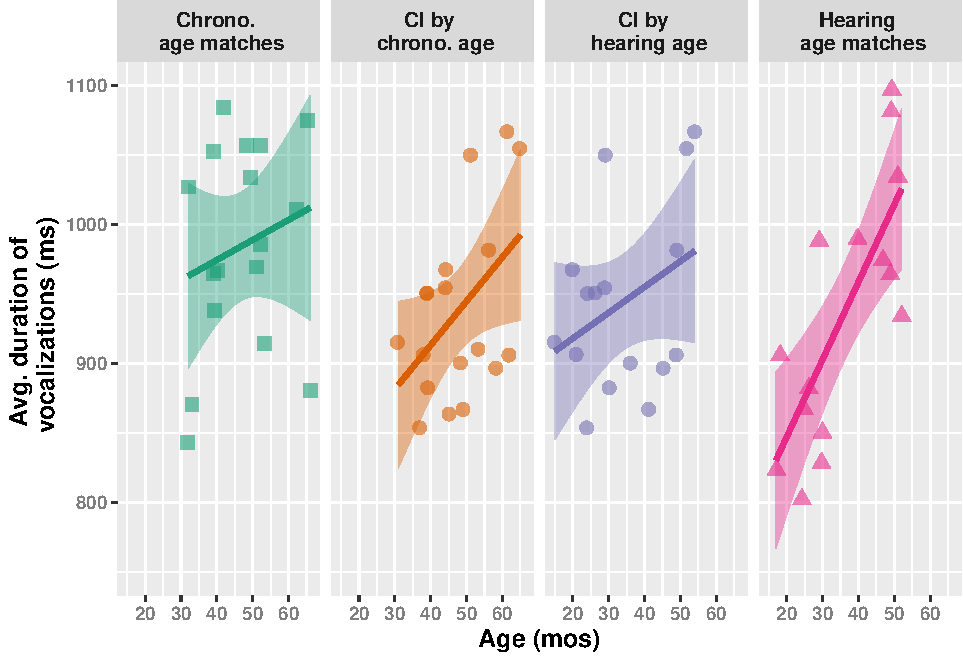
\includegraphics{everyday_CI_files/figure-latex/visualize age and voc duration continuously-1.pdf}

\begin{Shaded}
\begin{Highlighting}[]
\NormalTok{its\_df }\SpecialCharTok{\%\textgreater{}\%}
  \FunctionTok{select}\NormalTok{(child\_id, age\_mos) }\SpecialCharTok{\%\textgreater{}\%}
  \FunctionTok{merge}\NormalTok{(., recording\_vocs, }\AttributeTok{by=}\StringTok{\textquotesingle{}child\_id\textquotesingle{}}\NormalTok{) }\SpecialCharTok{\%\textgreater{}\%}
  \FunctionTok{rbind}\NormalTok{(., ha\_kids) }\SpecialCharTok{\%\textgreater{}\%}
  \FunctionTok{mutate}\NormalTok{(}\AttributeTok{match=}\FunctionTok{recode}\NormalTok{(match,}
                      \AttributeTok{chrono=}\StringTok{\textquotesingle{}Chrono. }\SpecialCharTok{\textbackslash{}n}\StringTok{ age matches\textquotesingle{}}\NormalTok{,}
                      \AttributeTok{CI=}\StringTok{\textquotesingle{}CI by }\SpecialCharTok{\textbackslash{}n}\StringTok{ chrono. age\textquotesingle{}}\NormalTok{,}
                      \AttributeTok{CI\_by\_hearing\_age=}\StringTok{\textquotesingle{}CI by }\SpecialCharTok{\textbackslash{}n}\StringTok{ hearing age\textquotesingle{}}\NormalTok{,}
                      \AttributeTok{HA=}\StringTok{\textquotesingle{}Hearing }\SpecialCharTok{\textbackslash{}n}\StringTok{ age matches\textquotesingle{}}\NormalTok{)) }\SpecialCharTok{\%\textgreater{}\%}
\FunctionTok{ggplot}\NormalTok{(., }\FunctionTok{aes}\NormalTok{(age\_mos, normed\_vocs)) }\SpecialCharTok{+}
  \FunctionTok{geom\_jitter}\NormalTok{(}\FunctionTok{aes}\NormalTok{(}\AttributeTok{color=}\NormalTok{match, }\AttributeTok{fill=}\NormalTok{match, }\AttributeTok{shape=}\NormalTok{match),}\AttributeTok{size=}\FloatTok{2.8}\NormalTok{,}\AttributeTok{alpha=}\NormalTok{.}\DecValTok{6}\NormalTok{,}\AttributeTok{width =}\NormalTok{ .}\DecValTok{3}\NormalTok{) }\SpecialCharTok{+}
  \FunctionTok{geom\_smooth}\NormalTok{(}\FunctionTok{aes}\NormalTok{(}\AttributeTok{fill=}\NormalTok{match, }\AttributeTok{color=}\NormalTok{match), }\AttributeTok{method =} \StringTok{"lm"}\NormalTok{,}\AttributeTok{size=}\FloatTok{1.2}\NormalTok{) }\SpecialCharTok{+}
  \FunctionTok{scale\_shape\_manual}\NormalTok{(}\AttributeTok{values=}\FunctionTok{c}\NormalTok{(}\DecValTok{15}\NormalTok{,}\DecValTok{16}\NormalTok{,}\DecValTok{16}\NormalTok{,}\DecValTok{17}\NormalTok{)) }\SpecialCharTok{+}
  \FunctionTok{facet\_grid}\NormalTok{(}\SpecialCharTok{\textasciitilde{}}\NormalTok{match) }\SpecialCharTok{+}
  \FunctionTok{scale\_color\_brewer}\NormalTok{(}\AttributeTok{palette=}\StringTok{"Dark2"}\NormalTok{) }\SpecialCharTok{+}
  \FunctionTok{scale\_fill\_brewer}\NormalTok{(}\AttributeTok{palette=}\StringTok{"Dark2"}\NormalTok{) }\SpecialCharTok{+}
  \FunctionTok{xlab}\NormalTok{(}\StringTok{"Age (mos)"}\NormalTok{) }\SpecialCharTok{+}
  \FunctionTok{ylab}\NormalTok{(}\StringTok{"Avg. \# of }\SpecialCharTok{\textbackslash{}n}\StringTok{ vocalizations/hr"}\NormalTok{) }\SpecialCharTok{+} 
    \FunctionTok{theme}\NormalTok{(}\AttributeTok{axis.title =} \FunctionTok{element\_text}\NormalTok{(}\AttributeTok{face =}\StringTok{"bold"}\NormalTok{, }\AttributeTok{size=}\DecValTok{12}\NormalTok{),}
        \AttributeTok{legend.position =} \StringTok{"none"}\NormalTok{, }
        \AttributeTok{axis.text =} \FunctionTok{element\_text}\NormalTok{(}\AttributeTok{face=}\StringTok{"bold"}\NormalTok{, }\AttributeTok{color=}\StringTok{\textquotesingle{}gray50\textquotesingle{}}\NormalTok{, }\AttributeTok{size=}\DecValTok{9}\NormalTok{),}
        \AttributeTok{strip.text=}\FunctionTok{element\_text}\NormalTok{(}\AttributeTok{face=}\StringTok{\textquotesingle{}bold\textquotesingle{}}\NormalTok{, }\AttributeTok{size=}\DecValTok{10}\NormalTok{))}
\end{Highlighting}
\end{Shaded}

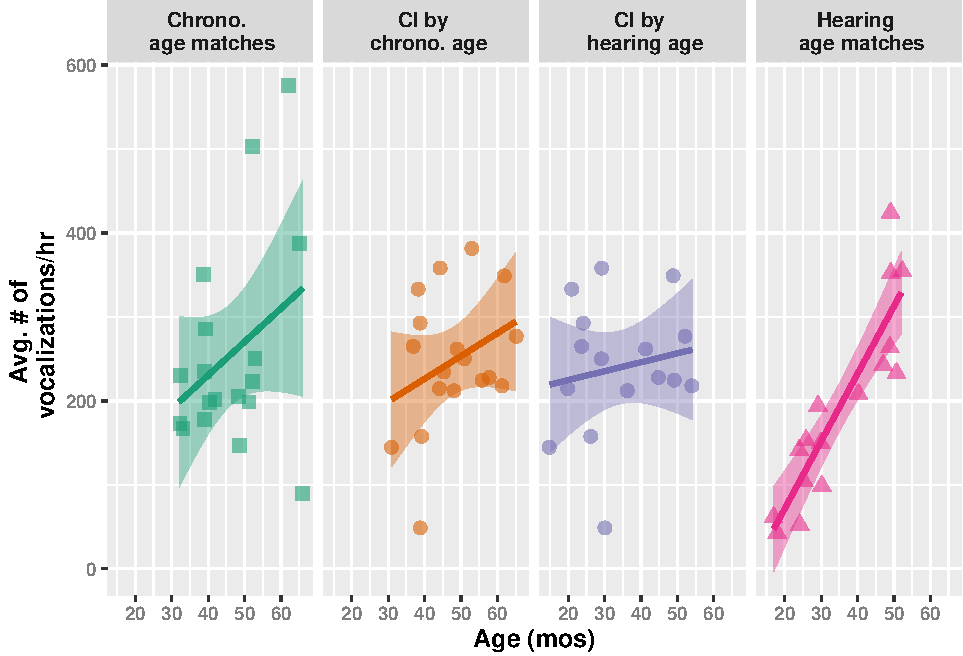
\includegraphics{everyday_CI_files/figure-latex/visualize age and voc quantity continuously-1.pdf}

\hypertarget{model-vocalizations}{%
\subsection{Model vocalizations}\label{model-vocalizations}}

\begin{Shaded}
\begin{Highlighting}[]
\CommentTok{\# {-}{-}{-}{-}{-}{-}{-}{-}{-}{-} QUANTITY {-}{-}{-}{-}{-}{-}{-}{-}{-}{-}{-}{-}}
\CommentTok{\# repeated measures}
\CommentTok{\# intensity}
\NormalTok{vocs}\SpecialCharTok{$}\NormalTok{match }\OtherTok{\textless{}{-}} \FunctionTok{relevel}\NormalTok{(}\FunctionTok{factor}\NormalTok{(vocs}\SpecialCharTok{$}\NormalTok{match), }\AttributeTok{ref =} \StringTok{"CI"}\NormalTok{)}
\NormalTok{voc\_intensity\_m0 }\OtherTok{\textless{}{-}} \FunctionTok{lmer}\NormalTok{(avg\_dB}\SpecialCharTok{\textasciitilde{}} \SpecialCharTok{+}\NormalTok{ (}\DecValTok{1} \SpecialCharTok{|}\NormalTok{ child\_id), }\AttributeTok{data=}\NormalTok{vocs)}
\NormalTok{voc\_intensity\_m1 }\OtherTok{\textless{}{-}} \FunctionTok{lmer}\NormalTok{(avg\_dB}\SpecialCharTok{\textasciitilde{}}\NormalTok{match }\SpecialCharTok{+}\NormalTok{ (}\DecValTok{1} \SpecialCharTok{|}\NormalTok{ child\_id), }\AttributeTok{data=}\NormalTok{vocs)}
\FunctionTok{anova}\NormalTok{(voc\_intensity\_m0,voc\_intensity\_m1)}
\end{Highlighting}
\end{Shaded}

\begin{verbatim}
## Data: vocs
## Models:
## voc_intensity_m0: avg_dB ~ +(1 | child_id)
## voc_intensity_m1: avg_dB ~ match + (1 | child_id)
##                  npar    AIC    BIC  logLik deviance  Chisq Df Pr(>Chisq)
## voc_intensity_m0    3 963736 963766 -481865   963730                     
## voc_intensity_m1    5 963739 963789 -481865   963729 0.6216  2     0.7329
\end{verbatim}

\begin{Shaded}
\begin{Highlighting}[]
\CommentTok{\# duration}
\NormalTok{hourly\_vocLen\_m0 }\OtherTok{\textless{}{-}} \FunctionTok{lmer}\NormalTok{(childUttLen}\SpecialCharTok{*}\DecValTok{1000}\SpecialCharTok{\textasciitilde{}} \SpecialCharTok{+}\NormalTok{ (}\DecValTok{1} \SpecialCharTok{|}\NormalTok{ child\_id), }\AttributeTok{data=}\NormalTok{vocs)}
\NormalTok{hourly\_vocLen\_m1 }\OtherTok{\textless{}{-}} \FunctionTok{lmer}\NormalTok{(childUttLen}\SpecialCharTok{*}\DecValTok{1000}\SpecialCharTok{\textasciitilde{}}\NormalTok{ match}\SpecialCharTok{+}\NormalTok{ (}\DecValTok{1} \SpecialCharTok{|}\NormalTok{ child\_id), }\AttributeTok{data=}\NormalTok{vocs)}
\FunctionTok{anova}\NormalTok{(hourly\_vocLen\_m0,hourly\_vocLen\_m1)}
\end{Highlighting}
\end{Shaded}

\begin{verbatim}
## Data: vocs
## Models:
## hourly_vocLen_m0: childUttLen * 1000 ~ +(1 | child_id)
## hourly_vocLen_m1: childUttLen * 1000 ~ match + (1 | child_id)
##                  npar     AIC     BIC   logLik deviance  Chisq Df Pr(>Chisq)  
## hourly_vocLen_m0    3 2620905 2620935 -1310450  2620899                       
## hourly_vocLen_m1    5 2620902 2620952 -1310446  2620892 6.9481  2    0.03099 *
## ---
## Signif. codes:  0 '***' 0.001 '**' 0.01 '*' 0.05 '.' 0.1 ' ' 1
\end{verbatim}

\begin{Shaded}
\begin{Highlighting}[]
\FunctionTok{summary}\NormalTok{(hourly\_vocLen\_m1)}
\end{Highlighting}
\end{Shaded}

\begin{verbatim}
## Linear mixed model fit by REML. t-tests use Satterthwaite's method [
## lmerModLmerTest]
## Formula: childUttLen * 1000 ~ match + (1 | child_id)
##    Data: vocs
## 
## REML criterion at convergence: 2620868
## 
## Scaled residuals: 
##     Min      1Q  Median      3Q     Max 
## -1.8378 -0.5909 -0.2715  0.2922 30.3097 
## 
## Random effects:
##  Groups   Name        Variance Std.Dev.
##  child_id (Intercept)   8178    90.43  
##  Residual             377986   614.81  
## Number of obs: 167130, groups:  child_id, 52
## 
## Fixed effects:
##             Estimate Std. Error     df t value Pr(>|t|)    
## (Intercept)   937.56      21.49  48.25   43.64   <2e-16 ***
## matchchrono    59.25      30.38  48.24    1.95    0.057 .  
## matchHA       -19.46      31.40  48.74   -0.62    0.538    
## ---
## Signif. codes:  0 '***' 0.001 '**' 0.01 '*' 0.05 '.' 0.1 ' ' 1
## 
## Correlation of Fixed Effects:
##             (Intr) mtchch
## matchchrono -0.707       
## matchHA     -0.684  0.484
\end{verbatim}

\begin{Shaded}
\begin{Highlighting}[]
\CommentTok{\# hourly measures }
\NormalTok{hourly\_vocs}\SpecialCharTok{$}\NormalTok{match }\OtherTok{\textless{}{-}} \FunctionTok{relevel}\NormalTok{(}\FunctionTok{factor}\NormalTok{(hourly\_vocs}\SpecialCharTok{$}\NormalTok{match), }\AttributeTok{ref =} \StringTok{"CI"}\NormalTok{)}
\NormalTok{hourly\_vocs}\SpecialCharTok{$}\NormalTok{hours }\OtherTok{\textless{}{-}} \FunctionTok{as.factor}\NormalTok{(hourly\_vocs}\SpecialCharTok{$}\NormalTok{hours)}
\NormalTok{hourly\_vocs\_m0 }\OtherTok{\textless{}{-}} \FunctionTok{lmer}\NormalTok{(normed\_hourly\_vocs}\SpecialCharTok{\textasciitilde{}} \SpecialCharTok{+}\NormalTok{ (}\DecValTok{1} \SpecialCharTok{|}\NormalTok{ child\_id) }\SpecialCharTok{+}\NormalTok{ (}\DecValTok{1}\SpecialCharTok{|}\NormalTok{hours), }\AttributeTok{data=}\NormalTok{hourly\_vocs)}
\NormalTok{hourly\_vocs\_m1 }\OtherTok{\textless{}{-}} \FunctionTok{lmer}\NormalTok{(normed\_hourly\_vocs}\SpecialCharTok{\textasciitilde{}}\NormalTok{ match}\SpecialCharTok{+}\NormalTok{ (}\DecValTok{1} \SpecialCharTok{|}\NormalTok{ child\_id) }\SpecialCharTok{+}\NormalTok{ (}\DecValTok{1}\SpecialCharTok{|}\NormalTok{hours), }\AttributeTok{data=}\NormalTok{hourly\_vocs)}
\FunctionTok{anova}\NormalTok{(hourly\_vocs\_m0,hourly\_vocs\_m1)}
\end{Highlighting}
\end{Shaded}

\begin{verbatim}
## Data: hourly_vocs
## Models:
## hourly_vocs_m0: normed_hourly_vocs ~ +(1 | child_id) + (1 | hours)
## hourly_vocs_m1: normed_hourly_vocs ~ match + (1 | child_id) + (1 | hours)
##                npar    AIC    BIC  logLik deviance  Chisq Df Pr(>Chisq)
## hourly_vocs_m0    4 8970.1 8988.1 -4481.0   8962.1                     
## hourly_vocs_m1    6 8971.8 8998.9 -4479.9   8959.8 2.2808  2     0.3197
\end{verbatim}

\begin{Shaded}
\begin{Highlighting}[]
\CommentTok{\# {-}{-}{-}{-}{-}{-}{-}{-}{-}{-} CONSISTENCY {-}{-}{-}{-}{-}{-}{-}{-}{-}{-}{-}{-}}
\NormalTok{voc\_consis2 }\OtherTok{\textless{}{-}}\NormalTok{ its\_df }\SpecialCharTok{\%\textgreater{}\%} \FunctionTok{select}\NormalTok{(age\_mos, child\_id) }\SpecialCharTok{\%\textgreater{}\%} \FunctionTok{merge}\NormalTok{(., voc\_consis, }\AttributeTok{by=}\StringTok{\textquotesingle{}child\_id\textquotesingle{}}\NormalTok{)}
\NormalTok{voc\_consis2}\SpecialCharTok{$}\NormalTok{match }\OtherTok{\textless{}{-}} \FunctionTok{relevel}\NormalTok{(}\FunctionTok{factor}\NormalTok{(voc\_consis2}\SpecialCharTok{$}\NormalTok{match), }\AttributeTok{ref =} \StringTok{"CI"}\NormalTok{)}
\NormalTok{voc\_consis\_m0 }\OtherTok{\textless{}{-}} \FunctionTok{lm}\NormalTok{(perc\_vocs}\SpecialCharTok{\textasciitilde{}}\NormalTok{age\_mos, }\AttributeTok{data=}\NormalTok{voc\_consis2)}
\NormalTok{voc\_consis\_m1 }\OtherTok{\textless{}{-}} \FunctionTok{lm}\NormalTok{(perc\_vocs}\SpecialCharTok{\textasciitilde{}}\NormalTok{ age\_mos }\SpecialCharTok{+}\NormalTok{ match, }\AttributeTok{data=}\NormalTok{voc\_consis2)}
\FunctionTok{anova}\NormalTok{(voc\_consis\_m0,voc\_consis\_m1) }\CommentTok{\# no}
\end{Highlighting}
\end{Shaded}

\begin{verbatim}
## Analysis of Variance Table
## 
## Model 1: perc_vocs ~ age_mos
## Model 2: perc_vocs ~ age_mos + match
##   Res.Df     RSS Df Sum of Sq      F Pr(>F)
## 1     50 0.79041                           
## 2     48 0.78237  2 0.0080337 0.2464 0.7826
\end{verbatim}

\begin{Shaded}
\begin{Highlighting}[]
\NormalTok{voc\_consis\_m2 }\OtherTok{\textless{}{-}} \FunctionTok{lm}\NormalTok{(perc\_vocs}\SpecialCharTok{\textasciitilde{}}\NormalTok{ age\_mos}\SpecialCharTok{*}\NormalTok{match, }\AttributeTok{data=}\NormalTok{voc\_consis2)}
\FunctionTok{anova}\NormalTok{(voc\_consis\_m0,voc\_consis\_m2) }\CommentTok{\# no}
\end{Highlighting}
\end{Shaded}

\begin{verbatim}
## Analysis of Variance Table
## 
## Model 1: perc_vocs ~ age_mos
## Model 2: perc_vocs ~ age_mos * match
##   Res.Df     RSS Df Sum of Sq      F Pr(>F)
## 1     50 0.79041                           
## 2     46 0.71175  4  0.078656 1.2709 0.2951
\end{verbatim}

\hypertarget{input-analyses}{%
\section{Input analyses}\label{input-analyses}}

\hypertarget{compute-input-statistics-and-make-tables}{%
\subsection{Compute input statistics and make tables}\label{compute-input-statistics-and-make-tables}}

\begin{Shaded}
\begin{Highlighting}[]
\CommentTok{\# summary statistics for each child }
\NormalTok{recording\_speech }\OtherTok{\textless{}{-}}\NormalTok{ speech }\SpecialCharTok{\%\textgreater{}\%}
  \FunctionTok{group\_by}\NormalTok{(match, child\_id) }\SpecialCharTok{\%\textgreater{}\%}
  \FunctionTok{summarize}\NormalTok{(}\AttributeTok{normed\_words =} \FunctionTok{sum}\NormalTok{(wordCount)}\SpecialCharTok{/}\NormalTok{total\_hrs, }\CommentTok{\# avg. number of words/hr}
            \AttributeTok{normed\_speech =} \FunctionTok{sum}\NormalTok{(duration)}\SpecialCharTok{/}\NormalTok{total\_hrs) }\SpecialCharTok{\%\textgreater{}\%}  \CommentTok{\# avg. \# of seconds of speech/hr}
  \FunctionTok{distinct}\NormalTok{(child\_id, }\AttributeTok{.keep\_all =}\NormalTok{ T) }

\NormalTok{prep\_speech\_quantity\_tbl }\OtherTok{\textless{}{-}}\NormalTok{ recording\_speech }\SpecialCharTok{\%\textgreater{}\%}
  \FunctionTok{group\_by}\NormalTok{(match) }\SpecialCharTok{\%\textgreater{}\%}
  \FunctionTok{summarize}\NormalTok{(}\AttributeTok{mean\_normed\_words =} \FunctionTok{mean}\NormalTok{(normed\_words), }\CommentTok{\# avg. number of words/hr}
            \AttributeTok{sd\_normed\_words =} \FunctionTok{sd}\NormalTok{(normed\_words),}
            \AttributeTok{min\_normed\_words =} \FunctionTok{min}\NormalTok{(normed\_words),}
            \AttributeTok{max\_normed\_words =} \FunctionTok{max}\NormalTok{(normed\_words),}
            \AttributeTok{mean\_normed\_speech =} \FunctionTok{mean}\NormalTok{(normed\_speech),  }\CommentTok{\# avg. \# of seconds of speech/hr}
            \AttributeTok{sd\_normed\_speech =} \FunctionTok{sd}\NormalTok{(normed\_speech),}
            \AttributeTok{min\_normed\_speech =} \FunctionTok{min}\NormalTok{(normed\_speech),}
            \AttributeTok{max\_normed\_speech =} \FunctionTok{max}\NormalTok{(normed\_speech)) }\SpecialCharTok{\%\textgreater{}\%}
  \FunctionTok{mutate\_if}\NormalTok{(is.numeric, round, }\DecValTok{2}\NormalTok{)}

\NormalTok{intensity\_stat }\OtherTok{\textless{}{-}}\NormalTok{ speech }\SpecialCharTok{\%\textgreater{}\%}
  \FunctionTok{group\_by}\NormalTok{(match) }\SpecialCharTok{\%\textgreater{}\%}
  \FunctionTok{summarize}\NormalTok{(}\AttributeTok{mean\_dB =} \FunctionTok{mean}\NormalTok{(avg\_dB), }\CommentTok{\# group{-}level average}
            \AttributeTok{sd\_dB =} \FunctionTok{sd}\NormalTok{(avg\_dB), }\CommentTok{\# group{-}level variance}
            \AttributeTok{min\_dB =} \FunctionTok{min}\NormalTok{(avg\_dB),}
            \AttributeTok{max\_dB =} \FunctionTok{max}\NormalTok{(avg\_dB)) }\SpecialCharTok{\%\textgreater{}\%}
  \FunctionTok{mutate\_if}\NormalTok{(is.numeric, round, }\DecValTok{2}\NormalTok{)}

\NormalTok{word\_stat }\OtherTok{\textless{}{-}}\NormalTok{ prep\_speech\_quantity\_tbl }\SpecialCharTok{\%\textgreater{}\%}
  \FunctionTok{mutate}\NormalTok{(}\AttributeTok{word\_quantity =} \FunctionTok{paste0}\NormalTok{(mean\_normed\_words,}\StringTok{"("}\NormalTok{,}
\NormalTok{                                sd\_normed\_words,}\StringTok{")"}\NormalTok{,}\StringTok{","}\NormalTok{,}
\NormalTok{                                min\_normed\_words,}\StringTok{"{-}"}\NormalTok{,}
\NormalTok{                                max\_normed\_words)) }\SpecialCharTok{\%\textgreater{}\%}
  \FunctionTok{select}\NormalTok{(match, word\_quantity) }\SpecialCharTok{\%\textgreater{}\%}
  \FunctionTok{spread}\NormalTok{(match, word\_quantity)}

\NormalTok{speech\_stat }\OtherTok{\textless{}{-}}\NormalTok{ prep\_speech\_quantity\_tbl }\SpecialCharTok{\%\textgreater{}\%}
  \FunctionTok{mutate}\NormalTok{(}\AttributeTok{input\_quantity =} \FunctionTok{paste0}\NormalTok{(mean\_normed\_speech,}\StringTok{"("}\NormalTok{,}
\NormalTok{                                 sd\_normed\_speech,}\StringTok{")"}\NormalTok{,}\StringTok{","}\NormalTok{,}
\NormalTok{                                 min\_normed\_speech,}\StringTok{"{-}"}\NormalTok{,}
\NormalTok{                                 max\_normed\_speech)) }\SpecialCharTok{\%\textgreater{}\%}
  \FunctionTok{select}\NormalTok{(match, input\_quantity) }\SpecialCharTok{\%\textgreater{}\%}
  \FunctionTok{spread}\NormalTok{(match, input\_quantity)}

\NormalTok{speech\_quantity\_tbl }\OtherTok{\textless{}{-}}\NormalTok{ intensity\_stat }\SpecialCharTok{\%\textgreater{}\%}
  \FunctionTok{mutate}\NormalTok{(}\AttributeTok{input\_intensity =} \FunctionTok{paste0}\NormalTok{(mean\_dB,}\StringTok{"("}\NormalTok{,sd\_dB,}\StringTok{")"}\NormalTok{,}\StringTok{","}\NormalTok{,min\_dB,}\StringTok{"{-}"}\NormalTok{,max\_dB)) }\SpecialCharTok{\%\textgreater{}\%}
  \FunctionTok{select}\NormalTok{(match, input\_intensity) }\SpecialCharTok{\%\textgreater{}\%}
  \FunctionTok{spread}\NormalTok{(match, input\_intensity) }\SpecialCharTok{\%\textgreater{}\%}
  \FunctionTok{rbind}\NormalTok{(., word\_stat) }\SpecialCharTok{\%\textgreater{}\%}
  \FunctionTok{rbind}\NormalTok{(., speech\_stat) }\SpecialCharTok{\%\textgreater{}\%}
  \FunctionTok{rownames\_to\_column}\NormalTok{(.,}\AttributeTok{var =} \StringTok{\textquotesingle{}measure\textquotesingle{}}\NormalTok{) }\SpecialCharTok{\%\textgreater{}\%}
  \FunctionTok{mutate}\NormalTok{(}\AttributeTok{measure =} \FunctionTok{case\_when}\NormalTok{(measure}\SpecialCharTok{==}\StringTok{\textquotesingle{}1\textquotesingle{}}\SpecialCharTok{\textasciitilde{}}\StringTok{\textquotesingle{}intensity\textquotesingle{}}\NormalTok{,}
\NormalTok{            measure}\SpecialCharTok{==}\StringTok{\textquotesingle{}2\textquotesingle{}}\SpecialCharTok{\textasciitilde{}}\StringTok{\textquotesingle{}num\_words\_hr\textquotesingle{}}\NormalTok{,}
            \ConstantTok{TRUE}\SpecialCharTok{\textasciitilde{}}\StringTok{\textquotesingle{}mins\_speech\_hr\textquotesingle{}}\NormalTok{))}

  
\CommentTok{\# the num of words and amount of speech from adults for each child, for each hour of the day}
\CommentTok{\# hourly speech refers to the avg. num of seconds of speech input each hour}
\NormalTok{hourly\_speech }\OtherTok{\textless{}{-}}\NormalTok{ speech }\SpecialCharTok{\%\textgreater{}\%}
  \FunctionTok{group\_by}\NormalTok{(match, implanted, child\_id, age\_mos, hours) }\SpecialCharTok{\%\textgreater{}\%} 
  \FunctionTok{summarize}\NormalTok{(}\AttributeTok{normed\_hourly\_words =} \FunctionTok{sum}\NormalTok{(wordCount),}
            \AttributeTok{normed\_hourly\_speech =} \FunctionTok{sum}\NormalTok{(duration)) }\SpecialCharTok{\%\textgreater{}\%}
  \FunctionTok{filter}\NormalTok{(normed\_hourly\_speech}\SpecialCharTok{\textgreater{}}\DecValTok{3}\NormalTok{) }\CommentTok{\# remove all hours with less than 3 seconds of speech}

\CommentTok{\# now choose the highest vocal activity hour}
\CommentTok{\# for each child}
\NormalTok{high\_word\_hour }\OtherTok{\textless{}{-}}\NormalTok{ hourly\_speech }\SpecialCharTok{\%\textgreater{}\%}
  \FunctionTok{group\_by}\NormalTok{(child\_id) }\SpecialCharTok{\%\textgreater{}\%}
  \FunctionTok{arrange}\NormalTok{(}\FunctionTok{desc}\NormalTok{(normed\_hourly\_words)) }\SpecialCharTok{\%\textgreater{}\%}
  \FunctionTok{slice}\NormalTok{(}\AttributeTok{n=}\DecValTok{1}\NormalTok{) }\SpecialCharTok{\%\textgreater{}\%}
  \FunctionTok{select}\NormalTok{(}\SpecialCharTok{{-}}\NormalTok{normed\_hourly\_speech, }\SpecialCharTok{{-}}\NormalTok{hours)}

\NormalTok{high\_hour }\OtherTok{\textless{}{-}}\NormalTok{ hourly\_speech }\SpecialCharTok{\%\textgreater{}\%}
  \FunctionTok{group\_by}\NormalTok{(child\_id) }\SpecialCharTok{\%\textgreater{}\%}
  \FunctionTok{arrange}\NormalTok{(}\FunctionTok{desc}\NormalTok{(normed\_hourly\_speech)) }\SpecialCharTok{\%\textgreater{}\%}
  \FunctionTok{slice}\NormalTok{(}\AttributeTok{n=}\DecValTok{1}\NormalTok{) }\SpecialCharTok{\%\textgreater{}\%}
  \FunctionTok{select}\NormalTok{(}\SpecialCharTok{{-}}\NormalTok{normed\_hourly\_words, }\SpecialCharTok{{-}}\NormalTok{hours) }\SpecialCharTok{\%\textgreater{}\%}
  \FunctionTok{merge}\NormalTok{(., high\_word\_hour, }\AttributeTok{by=}\FunctionTok{c}\NormalTok{(}\StringTok{\textquotesingle{}child\_id\textquotesingle{}}\NormalTok{, }\StringTok{\textquotesingle{}match\textquotesingle{}}\NormalTok{))}
  
\CommentTok{\# summary statistics for each match }
\NormalTok{all\_speech\_quantity\_tbl }\OtherTok{\textless{}{-}}\NormalTok{ speech }\SpecialCharTok{\%\textgreater{}\%}
  \FunctionTok{group\_by}\NormalTok{(match, child\_id) }\SpecialCharTok{\%\textgreater{}\%}
  \FunctionTok{summarize}\NormalTok{(}\AttributeTok{normed\_words =} \FunctionTok{sum}\NormalTok{(wordCount)}\SpecialCharTok{/}\NormalTok{total\_hrs,}
            \AttributeTok{normed\_speech =} \FunctionTok{sum}\NormalTok{(duration)}\SpecialCharTok{/}\NormalTok{total\_hrs) }\SpecialCharTok{\%\textgreater{}\%}
  \FunctionTok{ungroup}\NormalTok{() }\SpecialCharTok{\%\textgreater{}\%}
  \FunctionTok{merge}\NormalTok{(., high\_hour, }\AttributeTok{by=}\FunctionTok{c}\NormalTok{(}\StringTok{\textquotesingle{}child\_id\textquotesingle{}}\NormalTok{, }\StringTok{\textquotesingle{}match\textquotesingle{}}\NormalTok{)) }\SpecialCharTok{\%\textgreater{}\%} \CommentTok{\# with info about the measures from the highest vocal hour}
  \FunctionTok{group\_by}\NormalTok{(match) }\SpecialCharTok{\%\textgreater{}\%}
  \FunctionTok{summarize}\NormalTok{(}\AttributeTok{avg\_highhour\_words =} \FunctionTok{mean}\NormalTok{(normed\_hourly\_words),}
            \AttributeTok{sd\_highhour\_words =} \FunctionTok{sd}\NormalTok{(normed\_hourly\_words),}
            \AttributeTok{avg\_highhour\_speech =} \FunctionTok{mean}\NormalTok{(normed\_hourly\_speech),}
            \AttributeTok{sd\_highhour\_speech =} \FunctionTok{mean}\NormalTok{(normed\_hourly\_speech),}
            \AttributeTok{avg\_normed\_words =} \FunctionTok{mean}\NormalTok{(normed\_words),}
            \AttributeTok{sd\_normed\_words =} \FunctionTok{sd}\NormalTok{(normed\_words),}
            \AttributeTok{avg\_normed\_speech =} \FunctionTok{mean}\NormalTok{(normed\_speech),}
            \AttributeTok{sd\_normed\_speech =} \FunctionTok{sd}\NormalTok{(normed\_speech))}

\FunctionTok{kable}\NormalTok{(all\_speech\_quantity\_tbl, }\AttributeTok{booktabs=}\NormalTok{T, }
              \AttributeTok{caption=} \StringTok{"Speech input statistics, by hearing group"}\NormalTok{,}
             \AttributeTok{row.names =} \ConstantTok{FALSE}\NormalTok{) }\SpecialCharTok{\%\textgreater{}\%} 
  \FunctionTok{kable\_styling}\NormalTok{() }\SpecialCharTok{\%\textgreater{}\%}
\NormalTok{  kableExtra}\SpecialCharTok{::}\FunctionTok{kable\_styling}\NormalTok{(}\AttributeTok{latex\_options =} \StringTok{"hold\_position"}\NormalTok{)}
\end{Highlighting}
\end{Shaded}

\begin{table}[!h]

\caption{(\#tab:compute input stats)Speech input statistics, by hearing group}
\centering
\begin{tabular}[t]{lrrrrrrrr}
\toprule
match & avg\_highhour\_words & sd\_highhour\_words & avg\_highhour\_speech & sd\_highhour\_speech & avg\_normed\_words & sd\_normed\_words & avg\_normed\_speech & sd\_normed\_speech\\
\midrule
chrono & 3567.413 & 850.8975 & 877.0062 & 877.0062 & 1286.700 & 458.5779 & 322.4906 & 114.5057\\
CI & 3617.534 & 1227.9349 & 875.6365 & 875.6365 & 1488.456 & 472.4644 & 366.6176 & 110.7382\\
HA & 3531.419 & 1042.9615 & 893.0836 & 893.0836 & 1371.799 & 374.3342 & 344.8410 & 87.6545\\
\bottomrule
\end{tabular}
\end{table}

\begin{Shaded}
\begin{Highlighting}[]
\CommentTok{\# compute the percentage of minutes in the child\textquotesingle{}s day with \textgreater{} 1 AW }

\NormalTok{time\_steps }\OtherTok{\textless{}{-}} \FunctionTok{rep}\NormalTok{(}\FunctionTok{seq}\NormalTok{(}\DecValTok{60}\NormalTok{,}\DecValTok{57600}\NormalTok{,}\DecValTok{60}\NormalTok{),}\AttributeTok{times=}\DecValTok{52}\NormalTok{) }\SpecialCharTok{\%\textgreater{}\%} \FunctionTok{as.data.frame}\NormalTok{() }
\NormalTok{time\_steps}\SpecialCharTok{$}\NormalTok{seconds }\OtherTok{\textless{}{-}}\NormalTok{ time\_steps}\SpecialCharTok{$}\NormalTok{.}
\NormalTok{ids }\OtherTok{\textless{}{-}}\NormalTok{ speech }\SpecialCharTok{\%\textgreater{}\%} \FunctionTok{distinct}\NormalTok{(child\_id) }
\NormalTok{ids\_repeat }\OtherTok{\textless{}{-}} \FunctionTok{rep}\NormalTok{(ids}\SpecialCharTok{$}\NormalTok{child\_id,}\DecValTok{960}\NormalTok{) }\SpecialCharTok{\%\textgreater{}\%} \FunctionTok{as.data.frame}\NormalTok{()}
\NormalTok{ids\_repeat}\SpecialCharTok{$}\NormalTok{child\_id }\OtherTok{\textless{}{-}}\NormalTok{ ids\_repeat}\SpecialCharTok{$}\NormalTok{.}
\NormalTok{time\_steps\_demo }\OtherTok{\textless{}{-}}\NormalTok{ ids\_repeat }\SpecialCharTok{\%\textgreater{}\%}
  \FunctionTok{arrange}\NormalTok{(child\_id) }\SpecialCharTok{\%\textgreater{}\%}
  \FunctionTok{select}\NormalTok{(}\SpecialCharTok{{-}}\NormalTok{.) }\SpecialCharTok{\%\textgreater{}\%}
  \FunctionTok{cbind}\NormalTok{(., time\_steps) }\SpecialCharTok{\%\textgreater{}\%}
  \FunctionTok{select}\NormalTok{(child\_id, seconds)}

\NormalTok{match\_info }\OtherTok{\textless{}{-}}\NormalTok{ matches }\SpecialCharTok{\%\textgreater{}\%} \FunctionTok{select}\NormalTok{(match, child\_id) }

\NormalTok{pre\_input\_consis }\OtherTok{\textless{}{-}}\NormalTok{ speech }\SpecialCharTok{\%\textgreater{}\%}
  \FunctionTok{select}\NormalTok{(child\_id, seconds, duration, wordCount, clip\_onset) }\SpecialCharTok{\%\textgreater{}\%} 
  \FunctionTok{merge}\NormalTok{(., time\_steps\_demo, }\AttributeTok{by=}\FunctionTok{c}\NormalTok{(}\StringTok{\textquotesingle{}seconds\textquotesingle{}}\NormalTok{, }\StringTok{\textquotesingle{}child\_id\textquotesingle{}}\NormalTok{),}\AttributeTok{all=}\ConstantTok{TRUE}\NormalTok{) }\SpecialCharTok{\%\textgreater{}\%} \CommentTok{\# impute the missing seconds}
  \FunctionTok{replace\_na}\NormalTok{(}\FunctionTok{list}\NormalTok{(}\AttributeTok{duration =} \DecValTok{0}\NormalTok{, }\AttributeTok{wordCount=}\DecValTok{0}\NormalTok{)) }\SpecialCharTok{\%\textgreater{}\%} \CommentTok{\# replace the imputed time stamps with 0 adult words and 0 duration}
  \FunctionTok{merge}\NormalTok{(., match\_info, }\AttributeTok{by=}\StringTok{\textquotesingle{}child\_id\textquotesingle{}}\NormalTok{) }\CommentTok{\# remerge to get complete df of addtl measures w/o na\textquotesingle{}s }

\NormalTok{input\_consis }\OtherTok{\textless{}{-}}\NormalTok{ pre\_input\_consis }\SpecialCharTok{\%\textgreater{}\%}
  \FunctionTok{group\_by}\NormalTok{(match, child\_id, seconds) }\SpecialCharTok{\%\textgreater{}\%}
  \FunctionTok{summarize}\NormalTok{(}\AttributeTok{adult\_words =} \FunctionTok{sum}\NormalTok{(wordCount)) }\SpecialCharTok{\%\textgreater{}\%}
  \FunctionTok{ungroup}\NormalTok{() }\SpecialCharTok{\%\textgreater{}\%}
  \FunctionTok{mutate}\NormalTok{(}\AttributeTok{contains\_words =} \FunctionTok{if\_else}\NormalTok{((adult\_words }\SpecialCharTok{\textgreater{}} \DecValTok{0}\NormalTok{), }\StringTok{\textquotesingle{}TRUE\textquotesingle{}}\NormalTok{, }\StringTok{\textquotesingle{}FALSE\textquotesingle{}}\NormalTok{)) }\SpecialCharTok{\%\textgreater{}\%} \CommentTok{\# boolean if it contains words}
  \FunctionTok{ungroup}\NormalTok{() }\SpecialCharTok{\%\textgreater{}\%}
  \FunctionTok{group\_by}\NormalTok{(child\_id, contains\_words) }\SpecialCharTok{\%\textgreater{}\%}
  \FunctionTok{tally}\NormalTok{() }\SpecialCharTok{\%\textgreater{}\%}
  \FunctionTok{mutate}\NormalTok{(}\AttributeTok{perc\_words =} \FunctionTok{if\_else}\NormalTok{(child\_id}\SpecialCharTok{==}\StringTok{\textquotesingle{}177RTP1\textquotesingle{}}\NormalTok{, n}\SpecialCharTok{/}\DecValTok{770}\NormalTok{, n}\SpecialCharTok{/}\DecValTok{960}\NormalTok{)) }\SpecialCharTok{\%\textgreater{}\%} \CommentTok{\#769.8 minutes in 12.83 hr recording; others have 960}
  \FunctionTok{filter}\NormalTok{(contains\_words}\SpecialCharTok{==}\StringTok{\textquotesingle{}TRUE\textquotesingle{}}\NormalTok{) }\SpecialCharTok{\%\textgreater{}\%}
  \FunctionTok{merge}\NormalTok{(., match\_info, }\AttributeTok{by=}\StringTok{\textquotesingle{}child\_id\textquotesingle{}}\NormalTok{) }

\NormalTok{speech\_consis\_tbl }\OtherTok{\textless{}{-}}\NormalTok{ input\_consis }\SpecialCharTok{\%\textgreater{}\%}
  \FunctionTok{group\_by}\NormalTok{(match) }\SpecialCharTok{\%\textgreater{}\%}
  \FunctionTok{summarize}\NormalTok{(}\AttributeTok{mean\_perc\_words =} \FunctionTok{mean}\NormalTok{(perc\_words),}
            \AttributeTok{sd\_perc\_words =} \FunctionTok{sd}\NormalTok{(perc\_words),}
            \AttributeTok{min\_perc\_words =} \FunctionTok{min}\NormalTok{(perc\_words),}
            \AttributeTok{max\_perc\_words =} \FunctionTok{max}\NormalTok{(perc\_words)) }\SpecialCharTok{\%\textgreater{}\%}
  \FunctionTok{mutate\_if}\NormalTok{(is.numeric, round, }\DecValTok{2}\NormalTok{) }\SpecialCharTok{\%\textgreater{}\%}
  \FunctionTok{mutate}\NormalTok{(}\AttributeTok{input\_consistency =} \FunctionTok{paste0}\NormalTok{(mean\_perc\_words,}\StringTok{"("}\NormalTok{,sd\_perc\_words,}\StringTok{")"}\NormalTok{,}\StringTok{","}\NormalTok{,min\_perc\_words,}\StringTok{"{-}"}\NormalTok{,max\_perc\_words)) }\SpecialCharTok{\%\textgreater{}\%}
  \FunctionTok{select}\NormalTok{(match, input\_consistency) }\SpecialCharTok{\%\textgreater{}\%}
  \FunctionTok{spread}\NormalTok{(match, input\_consistency) }\SpecialCharTok{\%\textgreater{}\%}
  \FunctionTok{rownames\_to\_column}\NormalTok{(.,}\AttributeTok{var =} \StringTok{\textquotesingle{}measure\textquotesingle{}}\NormalTok{)}
\end{Highlighting}
\end{Shaded}

\begin{Shaded}
\begin{Highlighting}[]
\CommentTok{\# create a 4th "match" of CI kids to compute hearing age}
\NormalTok{ha }\OtherTok{\textless{}{-}}\NormalTok{ matches }\SpecialCharTok{\%\textgreater{}\%} \FunctionTok{select}\NormalTok{(child\_id, hearing\_age)}
\NormalTok{ha\_speech }\OtherTok{\textless{}{-}}\NormalTok{ its\_df }\SpecialCharTok{\%\textgreater{}\%}
  \FunctionTok{select}\NormalTok{(child\_id, age\_mos) }\SpecialCharTok{\%\textgreater{}\%}
  \FunctionTok{merge}\NormalTok{(., recording\_speech, }\AttributeTok{by=}\FunctionTok{c}\NormalTok{(}\StringTok{\textquotesingle{}child\_id\textquotesingle{}}\NormalTok{)) }\SpecialCharTok{\%\textgreater{}\%}
  \FunctionTok{merge}\NormalTok{(., ha, }\AttributeTok{by=}\StringTok{\textquotesingle{}child\_id\textquotesingle{}}\NormalTok{) }\SpecialCharTok{\%\textgreater{}\%}
  \FunctionTok{filter}\NormalTok{(match}\SpecialCharTok{==}\StringTok{\textquotesingle{}CI\textquotesingle{}}\NormalTok{) }\SpecialCharTok{\%\textgreater{}\%}
  \FunctionTok{select}\NormalTok{(}\SpecialCharTok{{-}}\NormalTok{age\_mos, }\SpecialCharTok{{-}}\NormalTok{match) }\SpecialCharTok{\%\textgreater{}\%}
  \FunctionTok{mutate}\NormalTok{(}\AttributeTok{age\_mos =}\NormalTok{ hearing\_age,}
         \AttributeTok{match =} \StringTok{\textquotesingle{}CI\_by\_hearing\_age\textquotesingle{}}\NormalTok{) }\SpecialCharTok{\%\textgreater{}\%}
  \FunctionTok{filter}\NormalTok{(}\SpecialCharTok{!}\NormalTok{hearing\_age}\SpecialCharTok{\textless{}=}\DecValTok{12}\NormalTok{) }\SpecialCharTok{\%\textgreater{}\%}
  \FunctionTok{select}\NormalTok{(}\SpecialCharTok{{-}}\NormalTok{hearing\_age) }


\NormalTok{input\_growth\_tbl }\OtherTok{\textless{}{-}}\NormalTok{ its\_df }\SpecialCharTok{\%\textgreater{}\%}
  \FunctionTok{select}\NormalTok{(child\_id, age\_mos) }\SpecialCharTok{\%\textgreater{}\%}
  \FunctionTok{merge}\NormalTok{(., recording\_speech, }\AttributeTok{by=}\StringTok{\textquotesingle{}child\_id\textquotesingle{}}\NormalTok{) }\SpecialCharTok{\%\textgreater{}\%}
  \FunctionTok{rbind}\NormalTok{(., ha\_speech) }\SpecialCharTok{\%\textgreater{}\%}
  \FunctionTok{group\_by}\NormalTok{(match) }\SpecialCharTok{\%\textgreater{}\%}
  \FunctionTok{do}\NormalTok{(}\AttributeTok{speech\_growth =} \FunctionTok{lm}\NormalTok{(normed\_words}\SpecialCharTok{\textasciitilde{}}\NormalTok{age\_mos, }\AttributeTok{data=}\NormalTok{.),}
     \AttributeTok{mod2 =} \FunctionTok{cor}\NormalTok{(.}\SpecialCharTok{$}\NormalTok{normed\_words, .}\SpecialCharTok{$}\NormalTok{age\_mos, }\AttributeTok{method =} \StringTok{"pearson"}\NormalTok{)) }\SpecialCharTok{\%\textgreater{}\%}
  \FunctionTok{mutate}\NormalTok{(}\AttributeTok{slope =} \FunctionTok{summary}\NormalTok{(speech\_growth)}\SpecialCharTok{$}\NormalTok{coeff[}\DecValTok{2}\NormalTok{],}
         \AttributeTok{p\_value =} \FunctionTok{summary}\NormalTok{(speech\_growth)}\SpecialCharTok{$}\NormalTok{coeff[}\DecValTok{8}\NormalTok{],}
         \AttributeTok{Pearson =}\NormalTok{ mod2[}\DecValTok{1}\NormalTok{]) }\SpecialCharTok{\%\textgreater{}\%}
  \FunctionTok{select}\NormalTok{(match, slope, p\_value, Pearson) }\SpecialCharTok{\%\textgreater{}\%}
  \FunctionTok{mutate\_if}\NormalTok{(is.numeric, round, }\DecValTok{2}\NormalTok{) }\SpecialCharTok{\%\textgreater{}\%}
  \FunctionTok{mutate}\NormalTok{(}\AttributeTok{stats=}\FunctionTok{paste0}\NormalTok{(}\StringTok{\textquotesingle{}B=\textquotesingle{}}\NormalTok{,slope,}\StringTok{","}\NormalTok{,}\StringTok{"p="}\NormalTok{,p\_value, }\StringTok{","}\NormalTok{,}\StringTok{"r="}\NormalTok{, Pearson)) }\SpecialCharTok{\%\textgreater{}\%}
  \FunctionTok{select}\NormalTok{(}\SpecialCharTok{{-}}\NormalTok{slope, }\SpecialCharTok{{-}}\NormalTok{p\_value, }\SpecialCharTok{{-}}\NormalTok{Pearson) }\SpecialCharTok{\%\textgreater{}\%}
  \FunctionTok{spread}\NormalTok{(match, stats) }\SpecialCharTok{\%\textgreater{}\%}
  \FunctionTok{mutate}\NormalTok{(}\AttributeTok{measure=}\StringTok{\textquotesingle{}Adult word growth\textquotesingle{}}\NormalTok{) }
\end{Highlighting}
\end{Shaded}

\hypertarget{model-input}{%
\subsection{Model input}\label{model-input}}

\begin{Shaded}
\begin{Highlighting}[]
\CommentTok{\# {-}{-}{-}{-}{-}{-}{-}{-}{-}{-} QUANTITY {-}{-}{-}{-}{-}{-}{-}{-}{-}{-}{-}{-}}
\CommentTok{\# repeated measures}
\CommentTok{\# intensity}
\NormalTok{speech}\SpecialCharTok{$}\NormalTok{match }\OtherTok{\textless{}{-}} \FunctionTok{relevel}\NormalTok{(}\FunctionTok{factor}\NormalTok{(speech}\SpecialCharTok{$}\NormalTok{match), }\AttributeTok{ref =} \StringTok{"CI"}\NormalTok{)}
\NormalTok{speech\_intensity\_m0 }\OtherTok{\textless{}{-}} \FunctionTok{lmer}\NormalTok{(avg\_dB}\SpecialCharTok{\textasciitilde{}} \SpecialCharTok{+}\NormalTok{ (}\DecValTok{1} \SpecialCharTok{|}\NormalTok{ child\_id), }\AttributeTok{data=}\NormalTok{speech)}
\NormalTok{speech\_intensity\_m1 }\OtherTok{\textless{}{-}} \FunctionTok{lmer}\NormalTok{(avg\_dB}\SpecialCharTok{\textasciitilde{}}\NormalTok{match }\SpecialCharTok{+}\NormalTok{ (}\DecValTok{1} \SpecialCharTok{|}\NormalTok{ child\_id), }\AttributeTok{data=}\NormalTok{speech)}
\FunctionTok{anova}\NormalTok{(speech\_intensity\_m0,speech\_intensity\_m1)}
\end{Highlighting}
\end{Shaded}

\begin{verbatim}
## Data: speech
## Models:
## speech_intensity_m0: avg_dB ~ +(1 | child_id)
## speech_intensity_m1: avg_dB ~ match + (1 | child_id)
##                     npar     AIC     BIC  logLik deviance  Chisq Df Pr(>Chisq)
## speech_intensity_m0    3 1121616 1121646 -560805  1121610                     
## speech_intensity_m1    5 1121618 1121669 -560804  1121608 1.4138  2     0.4932
\end{verbatim}

\begin{Shaded}
\begin{Highlighting}[]
\NormalTok{speech\_intensity }\OtherTok{\textless{}{-}} \FunctionTok{lmer}\NormalTok{(avg\_dB}\SpecialCharTok{\textasciitilde{}}\NormalTok{match }\SpecialCharTok{+}\NormalTok{ (}\DecValTok{1} \SpecialCharTok{|}\NormalTok{ child\_id), }\AttributeTok{data=}\NormalTok{speech)}

\CommentTok{\# hourly measures }
\CommentTok{\# minutes}
\NormalTok{hourly\_speech}\SpecialCharTok{$}\NormalTok{match }\OtherTok{\textless{}{-}} \FunctionTok{relevel}\NormalTok{(}\FunctionTok{factor}\NormalTok{(hourly\_speech}\SpecialCharTok{$}\NormalTok{match), }\AttributeTok{ref =} \StringTok{"CI"}\NormalTok{)}
\NormalTok{hourly\_speech}\SpecialCharTok{$}\NormalTok{hours }\OtherTok{\textless{}{-}} \FunctionTok{as.factor}\NormalTok{(hourly\_speech}\SpecialCharTok{$}\NormalTok{hours)}
\NormalTok{hourly\_speech\_m0 }\OtherTok{\textless{}{-}} \FunctionTok{lmer}\NormalTok{(normed\_hourly\_speech}\SpecialCharTok{\textasciitilde{}} \SpecialCharTok{+}\NormalTok{ (}\DecValTok{1} \SpecialCharTok{|}\NormalTok{ child\_id) }\SpecialCharTok{+}\NormalTok{ (}\DecValTok{1}\SpecialCharTok{|}\NormalTok{hours), }\AttributeTok{data=}\NormalTok{hourly\_speech)}
\NormalTok{hourly\_speech\_m1 }\OtherTok{\textless{}{-}} \FunctionTok{lmer}\NormalTok{(normed\_hourly\_speech}\SpecialCharTok{\textasciitilde{}}\NormalTok{ match}\SpecialCharTok{+}\NormalTok{ (}\DecValTok{1} \SpecialCharTok{|}\NormalTok{ child\_id) }\SpecialCharTok{+}\NormalTok{ (}\DecValTok{1}\SpecialCharTok{|}\NormalTok{hours), }\AttributeTok{data=}\NormalTok{hourly\_speech)}
\FunctionTok{anova}\NormalTok{(hourly\_speech\_m0,hourly\_speech\_m1)}
\end{Highlighting}
\end{Shaded}

\begin{verbatim}
## Data: hourly_speech
## Models:
## hourly_speech_m0: normed_hourly_speech ~ +(1 | child_id) + (1 | hours)
## hourly_speech_m1: normed_hourly_speech ~ match + (1 | child_id) + (1 | hours)
##                  npar    AIC    BIC  logLik deviance Chisq Df Pr(>Chisq)
## hourly_speech_m0    4 9351.2 9369.3 -4671.6   9343.2                    
## hourly_speech_m1    6 9353.6 9380.7 -4670.8   9341.6 1.624  2      0.444
\end{verbatim}

\begin{Shaded}
\begin{Highlighting}[]
\NormalTok{hourly\_speech\_m2 }\OtherTok{\textless{}{-}} \FunctionTok{lmer}\NormalTok{(normed\_hourly\_speech}\SpecialCharTok{\textasciitilde{}}\NormalTok{ age\_mos}\SpecialCharTok{+}\NormalTok{ (}\DecValTok{1} \SpecialCharTok{|}\NormalTok{ child\_id) }\SpecialCharTok{+}\NormalTok{ (}\DecValTok{1}\SpecialCharTok{|}\NormalTok{hours), }\AttributeTok{data=}\NormalTok{hourly\_speech)}

\CommentTok{\# words}
\NormalTok{hourly\_mins\_m0 }\OtherTok{\textless{}{-}} \FunctionTok{lmer}\NormalTok{(normed\_hourly\_words}\SpecialCharTok{\textasciitilde{}} \SpecialCharTok{+}\NormalTok{ (}\DecValTok{1} \SpecialCharTok{|}\NormalTok{ child\_id) }\SpecialCharTok{+}\NormalTok{ (}\DecValTok{1}\SpecialCharTok{|}\NormalTok{hours), }\AttributeTok{data=}\NormalTok{hourly\_speech)}
\NormalTok{hourly\_mins\_m1 }\OtherTok{\textless{}{-}} \FunctionTok{lmer}\NormalTok{(normed\_hourly\_words}\SpecialCharTok{\textasciitilde{}}\NormalTok{ match}\SpecialCharTok{+}\NormalTok{ (}\DecValTok{1} \SpecialCharTok{|}\NormalTok{ child\_id) }\SpecialCharTok{+}\NormalTok{ (}\DecValTok{1}\SpecialCharTok{|}\NormalTok{hours), }\AttributeTok{data=}\NormalTok{hourly\_speech)}
\FunctionTok{anova}\NormalTok{(hourly\_mins\_m0,hourly\_mins\_m1)}
\end{Highlighting}
\end{Shaded}

\begin{verbatim}
## Data: hourly_speech
## Models:
## hourly_mins_m0: normed_hourly_words ~ +(1 | child_id) + (1 | hours)
## hourly_mins_m1: normed_hourly_words ~ match + (1 | child_id) + (1 | hours)
##                npar   AIC   BIC  logLik deviance  Chisq Df Pr(>Chisq)
## hourly_mins_m0    4 11250 11268 -5621.0    11242                     
## hourly_mins_m1    6 11253 11280 -5620.3    11241 1.4309  2      0.489
\end{verbatim}

\begin{Shaded}
\begin{Highlighting}[]
\CommentTok{\# does the overall amount of speech change as children age?}
\NormalTok{hourly\_mins\_m2 }\OtherTok{\textless{}{-}} \FunctionTok{lmer}\NormalTok{(normed\_hourly\_words}\SpecialCharTok{\textasciitilde{}}\NormalTok{ age\_mos}\SpecialCharTok{+}\NormalTok{ (}\DecValTok{1} \SpecialCharTok{|}\NormalTok{ child\_id) }\SpecialCharTok{+}\NormalTok{ (}\DecValTok{1}\SpecialCharTok{|}\NormalTok{hours), }\AttributeTok{data=}\NormalTok{hourly\_speech)}



\CommentTok{\# {-}{-}{-}{-}{-}{-}{-}{-}{-}{-} CONSISTENCY {-}{-}{-}{-}{-}{-}{-}{-}{-}{-}{-}{-}}
\NormalTok{input\_consis2 }\OtherTok{\textless{}{-}}\NormalTok{ its\_df }\SpecialCharTok{\%\textgreater{}\%} \FunctionTok{select}\NormalTok{(age\_mos, child\_id) }\SpecialCharTok{\%\textgreater{}\%} \FunctionTok{merge}\NormalTok{(., input\_consis, }\AttributeTok{by=}\StringTok{\textquotesingle{}child\_id\textquotesingle{}}\NormalTok{)}
\NormalTok{input\_consis2}\SpecialCharTok{$}\NormalTok{match }\OtherTok{\textless{}{-}} \FunctionTok{relevel}\NormalTok{(}\FunctionTok{factor}\NormalTok{(input\_consis2}\SpecialCharTok{$}\NormalTok{match), }\AttributeTok{ref =} \StringTok{"CI"}\NormalTok{)}
\NormalTok{speech\_consis\_m0 }\OtherTok{\textless{}{-}} \FunctionTok{lm}\NormalTok{(perc\_words}\SpecialCharTok{\textasciitilde{}}\NormalTok{age\_mos, }\AttributeTok{data=}\NormalTok{input\_consis2)}
\NormalTok{speech\_consis\_m1 }\OtherTok{\textless{}{-}} \FunctionTok{lm}\NormalTok{(perc\_words}\SpecialCharTok{\textasciitilde{}}\NormalTok{ age\_mos }\SpecialCharTok{+}\NormalTok{ match, }\AttributeTok{data=}\NormalTok{input\_consis2)}
\FunctionTok{anova}\NormalTok{(speech\_consis\_m0,speech\_consis\_m1) }\CommentTok{\# no}
\end{Highlighting}
\end{Shaded}

\begin{verbatim}
## Analysis of Variance Table
## 
## Model 1: perc_words ~ age_mos
## Model 2: perc_words ~ age_mos + match
##   Res.Df     RSS Df Sum of Sq      F Pr(>F)
## 1     50 0.57049                           
## 2     48 0.54406  2  0.026437 1.1662 0.3202
\end{verbatim}

\begin{Shaded}
\begin{Highlighting}[]
\NormalTok{speech\_consis\_m2 }\OtherTok{\textless{}{-}} \FunctionTok{lm}\NormalTok{(perc\_words}\SpecialCharTok{\textasciitilde{}}\NormalTok{ age\_mos}\SpecialCharTok{*}\NormalTok{match, }\AttributeTok{data=}\NormalTok{input\_consis2)}
\FunctionTok{anova}\NormalTok{(speech\_consis\_m0,speech\_consis\_m2) }\CommentTok{\# no}
\end{Highlighting}
\end{Shaded}

\begin{verbatim}
## Analysis of Variance Table
## 
## Model 1: perc_words ~ age_mos
## Model 2: perc_words ~ age_mos * match
##   Res.Df     RSS Df Sum of Sq      F Pr(>F)
## 1     50 0.57049                           
## 2     46 0.51661  4  0.053881 1.1994 0.3239
\end{verbatim}

\begin{Shaded}
\begin{Highlighting}[]
\CommentTok{\# minutes}

\CommentTok{\# words}
\end{Highlighting}
\end{Shaded}

\hypertarget{convo-turn-analyses}{%
\section{Convo turn analyses}\label{convo-turn-analyses}}

\hypertarget{compute-convo-turns}{%
\subsection{Compute convo turns}\label{compute-convo-turns}}

\begin{Shaded}
\begin{Highlighting}[]
\CommentTok{\# summary statistics for each child }
\NormalTok{recording\_convo }\OtherTok{\textless{}{-}}\NormalTok{ convo }\SpecialCharTok{\%\textgreater{}\%}
  \FunctionTok{group\_by}\NormalTok{(child\_id) }\SpecialCharTok{\%\textgreater{}\%}
  \FunctionTok{summarize}\NormalTok{(}\AttributeTok{normed\_turns =} \FunctionTok{sum}\NormalTok{(convo\_count)}\SpecialCharTok{/}\NormalTok{total\_hrs,}
            \AttributeTok{avg\_dur =} \FunctionTok{mean}\NormalTok{(convo\_count),}
            \AttributeTok{sd\_dur =} \FunctionTok{sd}\NormalTok{(convo\_count)) }\SpecialCharTok{\%\textgreater{}\%}
  \FunctionTok{distinct}\NormalTok{(child\_id, }\AttributeTok{.keep\_all =}\NormalTok{ T)}

\CommentTok{\# the num of vocalizations for each child, for each hour of the day}
\NormalTok{hourly\_turns }\OtherTok{\textless{}{-}}\NormalTok{ convo }\SpecialCharTok{\%\textgreater{}\%}
  \FunctionTok{group\_by}\NormalTok{(match, implanted, child\_id, hours) }\SpecialCharTok{\%\textgreater{}\%} 
  \FunctionTok{summarize}\NormalTok{(}\AttributeTok{normed\_hourly\_turns =} \FunctionTok{sum}\NormalTok{(convo\_count))}

\CommentTok{\# summary statistics for each match }
\NormalTok{turn\_quantity\_tbl }\OtherTok{\textless{}{-}}\NormalTok{ convo }\SpecialCharTok{\%\textgreater{}\%}
  \FunctionTok{group\_by}\NormalTok{(match, child\_id) }\SpecialCharTok{\%\textgreater{}\%}
  \FunctionTok{summarize}\NormalTok{(}\AttributeTok{normed\_turns =} \FunctionTok{sum}\NormalTok{(convo\_count)}\SpecialCharTok{/}\NormalTok{total\_hrs) }\SpecialCharTok{\%\textgreater{}\%}
  \FunctionTok{ungroup}\NormalTok{() }\SpecialCharTok{\%\textgreater{}\%}
  \FunctionTok{group\_by}\NormalTok{(match) }\SpecialCharTok{\%\textgreater{}\%}
  \FunctionTok{summarize}\NormalTok{(}\AttributeTok{avg\_normed\_turns =} \FunctionTok{mean}\NormalTok{(normed\_turns),}
            \AttributeTok{sd\_normed\_turns =} \FunctionTok{sd}\NormalTok{(normed\_turns),}
            \AttributeTok{min\_normed\_turns =} \FunctionTok{min}\NormalTok{(normed\_turns),}
            \AttributeTok{max\_normed\_turns =} \FunctionTok{max}\NormalTok{(normed\_turns)) }\SpecialCharTok{\%\textgreater{}\%}
  \FunctionTok{mutate\_if}\NormalTok{(is.numeric, round, }\DecValTok{2}\NormalTok{) }\SpecialCharTok{\%\textgreater{}\%}
  \FunctionTok{mutate}\NormalTok{(}\AttributeTok{turn\_quantity =} \FunctionTok{paste0}\NormalTok{(avg\_normed\_turns,}\StringTok{"("}\NormalTok{,sd\_normed\_turns,}\StringTok{")"}\NormalTok{,}\StringTok{","}\NormalTok{,min\_normed\_turns,}\StringTok{"{-}"}\NormalTok{,max\_normed\_turns)) }\SpecialCharTok{\%\textgreater{}\%}
  \FunctionTok{select}\NormalTok{(match, turn\_quantity) }\SpecialCharTok{\%\textgreater{}\%}
  \FunctionTok{spread}\NormalTok{(match, turn\_quantity) }\SpecialCharTok{\%\textgreater{}\%}
  \FunctionTok{rownames\_to\_column}\NormalTok{(.,}\AttributeTok{var =} \StringTok{\textquotesingle{}measure\textquotesingle{}}\NormalTok{)}
\end{Highlighting}
\end{Shaded}

\begin{Shaded}
\begin{Highlighting}[]
\CommentTok{\# compute the percentage of epochs (5{-}min chunks) in the child\textquotesingle{}s day with \textgreater{} 1 CT}
\NormalTok{time\_steps }\OtherTok{\textless{}{-}} \FunctionTok{rep}\NormalTok{(}\FunctionTok{seq}\NormalTok{(}\DecValTok{1}\NormalTok{,}\DecValTok{192}\NormalTok{,}\DecValTok{1}\NormalTok{),}\AttributeTok{times=}\DecValTok{52}\NormalTok{) }\SpecialCharTok{\%\textgreater{}\%} \FunctionTok{as.data.frame}\NormalTok{() }
\NormalTok{time\_steps}\SpecialCharTok{$}\NormalTok{epochs }\OtherTok{\textless{}{-}}\NormalTok{ time\_steps}\SpecialCharTok{$}\NormalTok{.}
\NormalTok{ids }\OtherTok{\textless{}{-}}\NormalTok{ convo }\SpecialCharTok{\%\textgreater{}\%} \FunctionTok{distinct}\NormalTok{(child\_id) }
\NormalTok{ids\_repeat }\OtherTok{\textless{}{-}} \FunctionTok{rep}\NormalTok{(ids}\SpecialCharTok{$}\NormalTok{child\_id,}\DecValTok{192}\NormalTok{) }\SpecialCharTok{\%\textgreater{}\%} \FunctionTok{as.data.frame}\NormalTok{()}
\NormalTok{ids\_repeat}\SpecialCharTok{$}\NormalTok{child\_id }\OtherTok{\textless{}{-}}\NormalTok{ ids\_repeat}\SpecialCharTok{$}\NormalTok{.}
\NormalTok{time\_steps\_demo }\OtherTok{\textless{}{-}}\NormalTok{ ids\_repeat }\SpecialCharTok{\%\textgreater{}\%}
  \FunctionTok{arrange}\NormalTok{(child\_id) }\SpecialCharTok{\%\textgreater{}\%}
  \FunctionTok{select}\NormalTok{(}\SpecialCharTok{{-}}\NormalTok{.) }\SpecialCharTok{\%\textgreater{}\%}
  \FunctionTok{cbind}\NormalTok{(., time\_steps) }\SpecialCharTok{\%\textgreater{}\%}
  \FunctionTok{select}\NormalTok{(child\_id, epochs)}

\NormalTok{pre\_convo\_consis }\OtherTok{\textless{}{-}}\NormalTok{ convo }\SpecialCharTok{\%\textgreater{}\%}
  \FunctionTok{mutate}\NormalTok{(}\AttributeTok{epochs=}\FunctionTok{floor}\NormalTok{(seconds}\SpecialCharTok{/}\DecValTok{300}\NormalTok{)) }\SpecialCharTok{\%\textgreater{}\%} \CommentTok{\#round down to the nearest integer}
  \FunctionTok{select}\NormalTok{(child\_id, epochs, seconds, convo\_count, clip\_onset) }\SpecialCharTok{\%\textgreater{}\%} 
  \FunctionTok{merge}\NormalTok{(., time\_steps\_demo, }\AttributeTok{by=}\FunctionTok{c}\NormalTok{(}\StringTok{\textquotesingle{}epochs\textquotesingle{}}\NormalTok{, }\StringTok{\textquotesingle{}child\_id\textquotesingle{}}\NormalTok{),}\AttributeTok{all=}\ConstantTok{TRUE}\NormalTok{) }\SpecialCharTok{\%\textgreater{}\%} \CommentTok{\# impute the missing epochs}
  \FunctionTok{replace\_na}\NormalTok{(}\FunctionTok{list}\NormalTok{(}\AttributeTok{convo\_count=}\DecValTok{0}\NormalTok{)) }\SpecialCharTok{\%\textgreater{}\%}
  \FunctionTok{merge}\NormalTok{(., match\_info, }\AttributeTok{by=}\StringTok{\textquotesingle{}child\_id\textquotesingle{}}\NormalTok{)}\CommentTok{\# remerge to get complete df of addtl measures w/o na\textquotesingle{}s }

\NormalTok{convo\_consis\_check }\OtherTok{\textless{}{-}}\NormalTok{ pre\_convo\_consis }\SpecialCharTok{\%\textgreater{}\%}
  \FunctionTok{group\_by}\NormalTok{(match, child\_id, epochs) }\SpecialCharTok{\%\textgreater{}\%}
  \FunctionTok{summarize}\NormalTok{(}\AttributeTok{turns =} \FunctionTok{sum}\NormalTok{(convo\_count)) }\SpecialCharTok{\%\textgreater{}\%}
  \FunctionTok{ungroup}\NormalTok{() }\SpecialCharTok{\%\textgreater{}\%}
  \FunctionTok{mutate}\NormalTok{(}\AttributeTok{contains\_turns =} \FunctionTok{if\_else}\NormalTok{((turns }\SpecialCharTok{\textgreater{}} \DecValTok{0}\NormalTok{), }\StringTok{\textquotesingle{}TRUE\textquotesingle{}}\NormalTok{, }\StringTok{\textquotesingle{}FALSE\textquotesingle{}}\NormalTok{)) }\SpecialCharTok{\%\textgreater{}\%} \CommentTok{\# boolean if it contains turns}
  \FunctionTok{ungroup}\NormalTok{() }\SpecialCharTok{\%\textgreater{}\%}
  \FunctionTok{group\_by}\NormalTok{(child\_id, contains\_turns) }\SpecialCharTok{\%\textgreater{}\%}
  \FunctionTok{tally}\NormalTok{() }\SpecialCharTok{\%\textgreater{}\%}
  \FunctionTok{mutate}\NormalTok{(}\AttributeTok{perc\_turns =} \FunctionTok{if\_else}\NormalTok{(child\_id}\SpecialCharTok{==}\StringTok{\textquotesingle{}177RTP1\textquotesingle{}}\NormalTok{, n}\SpecialCharTok{/}\DecValTok{154}\NormalTok{, n}\SpecialCharTok{/}\DecValTok{192}\NormalTok{)) }\SpecialCharTok{\%\textgreater{}\%} \CommentTok{\#153.96 epochs in 12.83 hr recording; others have 192 }
  \FunctionTok{filter}\NormalTok{(contains\_turns}\SpecialCharTok{==}\StringTok{\textquotesingle{}TRUE\textquotesingle{}}\NormalTok{) }\SpecialCharTok{\%\textgreater{}\%}
  \FunctionTok{merge}\NormalTok{(., match\_info, }\AttributeTok{by=}\StringTok{\textquotesingle{}child\_id\textquotesingle{}}\NormalTok{) }

\CommentTok{\# report stats for speech table}
\NormalTok{convo\_consis\_tbl }\OtherTok{\textless{}{-}}\NormalTok{ convo\_consis\_check }\SpecialCharTok{\%\textgreater{}\%}
  \FunctionTok{group\_by}\NormalTok{(match) }\SpecialCharTok{\%\textgreater{}\%}
  \FunctionTok{summarize}\NormalTok{(}\AttributeTok{avg\_convo\_consis =} \FunctionTok{mean}\NormalTok{(perc\_turns),}
            \AttributeTok{sd\_convo\_consis =} \FunctionTok{sd}\NormalTok{(perc\_turns),}
            \AttributeTok{min\_convo\_consis =} \FunctionTok{min}\NormalTok{(perc\_turns),}
            \AttributeTok{max\_convo\_consis =} \FunctionTok{max}\NormalTok{(perc\_turns)) }\SpecialCharTok{\%\textgreater{}\%}
  \FunctionTok{mutate\_if}\NormalTok{(is.numeric, round, }\DecValTok{2}\NormalTok{) }\SpecialCharTok{\%\textgreater{}\%}
  \FunctionTok{mutate}\NormalTok{(}\AttributeTok{convo\_consis=}\FunctionTok{paste0}\NormalTok{(avg\_convo\_consis,}\StringTok{"("}\NormalTok{,sd\_convo\_consis,}\StringTok{")"}\NormalTok{,}\StringTok{","}\NormalTok{,min\_convo\_consis,}\StringTok{"{-}"}\NormalTok{,max\_convo\_consis)) }\SpecialCharTok{\%\textgreater{}\%}
  \FunctionTok{select}\NormalTok{(match,convo\_consis) }\SpecialCharTok{\%\textgreater{}\%}
  \FunctionTok{spread}\NormalTok{(match, convo\_consis) }\SpecialCharTok{\%\textgreater{}\%}
  \FunctionTok{rownames\_to\_column}\NormalTok{(.,}\AttributeTok{var =} \StringTok{\textquotesingle{}measure\textquotesingle{}}\NormalTok{)}
\end{Highlighting}
\end{Shaded}

\begin{Shaded}
\begin{Highlighting}[]
\CommentTok{\# create a 4th "match" of CI kids to compute hearing age}
\NormalTok{match }\OtherTok{\textless{}{-}}\NormalTok{ matches }\SpecialCharTok{\%\textgreater{}\%} \FunctionTok{select}\NormalTok{(child\_id, match, hearing\_age)}

\NormalTok{ha\_kids\_ctc }\OtherTok{\textless{}{-}}\NormalTok{ its\_df }\SpecialCharTok{\%\textgreater{}\%}
  \FunctionTok{select}\NormalTok{(child\_id, age\_mos) }\SpecialCharTok{\%\textgreater{}\%}
  \FunctionTok{merge}\NormalTok{(., recording\_convo, }\AttributeTok{by=}\StringTok{\textquotesingle{}child\_id\textquotesingle{}}\NormalTok{) }\SpecialCharTok{\%\textgreater{}\%}
  \FunctionTok{merge}\NormalTok{(., match, }\AttributeTok{by=}\StringTok{\textquotesingle{}child\_id\textquotesingle{}}\NormalTok{) }\SpecialCharTok{\%\textgreater{}\%}
  \FunctionTok{filter}\NormalTok{(match}\SpecialCharTok{==}\StringTok{\textquotesingle{}CI\textquotesingle{}}\NormalTok{) }\SpecialCharTok{\%\textgreater{}\%}
  \FunctionTok{select}\NormalTok{(}\SpecialCharTok{{-}}\NormalTok{age\_mos, }\SpecialCharTok{{-}}\NormalTok{match) }\SpecialCharTok{\%\textgreater{}\%}
  \FunctionTok{mutate}\NormalTok{(}\AttributeTok{age\_mos =}\NormalTok{ hearing\_age,}
         \AttributeTok{match =} \StringTok{\textquotesingle{}CI\_by\_hearing\_age\textquotesingle{}}\NormalTok{) }\SpecialCharTok{\%\textgreater{}\%}
  \FunctionTok{filter}\NormalTok{(}\SpecialCharTok{!}\NormalTok{hearing\_age}\SpecialCharTok{\textless{}=}\DecValTok{12}\NormalTok{) }\SpecialCharTok{\%\textgreater{}\%}
  \FunctionTok{select}\NormalTok{(}\SpecialCharTok{{-}}\NormalTok{hearing\_age)}

\NormalTok{ctc\_growth\_tbl }\OtherTok{\textless{}{-}}\NormalTok{ its\_df }\SpecialCharTok{\%\textgreater{}\%}
  \FunctionTok{select}\NormalTok{(child\_id, age\_mos, match) }\SpecialCharTok{\%\textgreater{}\%}
  \FunctionTok{merge}\NormalTok{(., recording\_convo, }\AttributeTok{by=}\StringTok{\textquotesingle{}child\_id\textquotesingle{}}\NormalTok{) }\SpecialCharTok{\%\textgreater{}\%}
  \FunctionTok{rbind}\NormalTok{(., ha\_kids\_ctc) }\SpecialCharTok{\%\textgreater{}\%}
  \FunctionTok{group\_by}\NormalTok{(match) }\SpecialCharTok{\%\textgreater{}\%}
  \FunctionTok{do}\NormalTok{(}\AttributeTok{ctc\_growth =} \FunctionTok{lm}\NormalTok{(normed\_turns}\SpecialCharTok{\textasciitilde{}}\NormalTok{age\_mos, }\AttributeTok{data=}\NormalTok{.),}
     \AttributeTok{mod2 =} \FunctionTok{cor}\NormalTok{(.}\SpecialCharTok{$}\NormalTok{normed\_turns, .}\SpecialCharTok{$}\NormalTok{age\_mos, }\AttributeTok{method =} \StringTok{"pearson"}\NormalTok{)) }\SpecialCharTok{\%\textgreater{}\%}
  \FunctionTok{mutate}\NormalTok{(}\AttributeTok{slope =} \FunctionTok{summary}\NormalTok{(ctc\_growth)}\SpecialCharTok{$}\NormalTok{coeff[}\DecValTok{2}\NormalTok{],}
         \AttributeTok{p\_value =} \FunctionTok{summary}\NormalTok{(ctc\_growth)}\SpecialCharTok{$}\NormalTok{coeff[}\DecValTok{8}\NormalTok{],}
         \AttributeTok{Pearson =}\NormalTok{ mod2[}\DecValTok{1}\NormalTok{]) }\SpecialCharTok{\%\textgreater{}\%}
  \FunctionTok{select}\NormalTok{(match, slope, p\_value, Pearson) }\SpecialCharTok{\%\textgreater{}\%}
  \FunctionTok{mutate\_if}\NormalTok{(is.numeric, round, }\DecValTok{2}\NormalTok{) }\SpecialCharTok{\%\textgreater{}\%}
  \FunctionTok{mutate}\NormalTok{(}\AttributeTok{stats=}\FunctionTok{paste0}\NormalTok{(}\StringTok{\textquotesingle{}B=\textquotesingle{}}\NormalTok{,slope,}\StringTok{","}\NormalTok{,}\StringTok{"p="}\NormalTok{,p\_value, }\StringTok{","}\NormalTok{,}\StringTok{"r="}\NormalTok{, Pearson)) }\SpecialCharTok{\%\textgreater{}\%}
  \FunctionTok{select}\NormalTok{(}\SpecialCharTok{{-}}\NormalTok{slope, }\SpecialCharTok{{-}}\NormalTok{p\_value, }\SpecialCharTok{{-}}\NormalTok{Pearson) }\SpecialCharTok{\%\textgreater{}\%}
  \FunctionTok{spread}\NormalTok{(match, stats) }\SpecialCharTok{\%\textgreater{}\%}
  \FunctionTok{mutate}\NormalTok{(}\AttributeTok{measure=}\StringTok{\textquotesingle{}Convo. turn growth\textquotesingle{}}\NormalTok{) }
\end{Highlighting}
\end{Shaded}

\hypertarget{model-turns}{%
\subsection{Model turns}\label{model-turns}}

\begin{Shaded}
\begin{Highlighting}[]
\CommentTok{\# {-}{-}{-}{-}{-}{-}{-}{-}{-}{-} QUANTITY {-}{-}{-}{-}{-}{-}{-}{-}{-}{-}{-}{-}}
\CommentTok{\# hourly measures }
\CommentTok{\# turns}
\NormalTok{hourly\_turns}\SpecialCharTok{$}\NormalTok{match }\OtherTok{\textless{}{-}} \FunctionTok{relevel}\NormalTok{(}\FunctionTok{factor}\NormalTok{(hourly\_turns}\SpecialCharTok{$}\NormalTok{match), }\AttributeTok{ref =} \StringTok{"CI"}\NormalTok{)}
\NormalTok{hourly\_turns}\SpecialCharTok{$}\NormalTok{hours }\OtherTok{\textless{}{-}} \FunctionTok{as.factor}\NormalTok{(hourly\_turns}\SpecialCharTok{$}\NormalTok{hours)}
\NormalTok{hourly\_turns\_m0 }\OtherTok{\textless{}{-}} \FunctionTok{lmer}\NormalTok{(normed\_hourly\_turns}\SpecialCharTok{\textasciitilde{}} \SpecialCharTok{+}\NormalTok{ (}\DecValTok{1} \SpecialCharTok{|}\NormalTok{ child\_id) }\SpecialCharTok{+}\NormalTok{ (}\DecValTok{1}\SpecialCharTok{|}\NormalTok{hours), }\AttributeTok{data=}\NormalTok{hourly\_turns)}
\NormalTok{hourly\_turns\_m1 }\OtherTok{\textless{}{-}} \FunctionTok{lmer}\NormalTok{(normed\_hourly\_turns}\SpecialCharTok{\textasciitilde{}}\NormalTok{ match}\SpecialCharTok{+}\NormalTok{ (}\DecValTok{1} \SpecialCharTok{|}\NormalTok{ child\_id) }\SpecialCharTok{+}\NormalTok{ (}\DecValTok{1}\SpecialCharTok{|}\NormalTok{hours), }\AttributeTok{data=}\NormalTok{hourly\_turns)}
\FunctionTok{anova}\NormalTok{(hourly\_turns\_m0,hourly\_turns\_m1)}
\end{Highlighting}
\end{Shaded}

\begin{verbatim}
## Data: hourly_turns
## Models:
## hourly_turns_m0: normed_hourly_turns ~ +(1 | child_id) + (1 | hours)
## hourly_turns_m1: normed_hourly_turns ~ match + (1 | child_id) + (1 | hours)
##                 npar    AIC    BIC  logLik deviance  Chisq Df Pr(>Chisq)
## hourly_turns_m0    4 6959.5 6977.4 -3475.7   6951.5                     
## hourly_turns_m1    6 6963.2 6990.1 -3475.6   6951.2 0.3015  2     0.8601
\end{verbatim}

\begin{Shaded}
\begin{Highlighting}[]
\CommentTok{\# {-}{-}{-}{-}{-}{-}{-}{-}{-}{-} CONSISTENCY {-}{-}{-}{-}{-}{-}{-}{-}{-}{-}{-}{-}}
\NormalTok{convo\_consis\_check2 }\OtherTok{\textless{}{-}}\NormalTok{ its\_df }\SpecialCharTok{\%\textgreater{}\%} \FunctionTok{select}\NormalTok{(age\_mos, child\_id) }\SpecialCharTok{\%\textgreater{}\%} \FunctionTok{merge}\NormalTok{(., convo\_consis\_check, }\AttributeTok{by=}\StringTok{\textquotesingle{}child\_id\textquotesingle{}}\NormalTok{)}
\NormalTok{convo\_consis\_check2}\SpecialCharTok{$}\NormalTok{match }\OtherTok{\textless{}{-}} \FunctionTok{relevel}\NormalTok{(}\FunctionTok{factor}\NormalTok{(convo\_consis\_check2}\SpecialCharTok{$}\NormalTok{match), }\AttributeTok{ref =} \StringTok{"CI"}\NormalTok{)}
\NormalTok{convo\_consis\_m0 }\OtherTok{\textless{}{-}} \FunctionTok{lm}\NormalTok{(perc\_turns}\SpecialCharTok{\textasciitilde{}}\NormalTok{age\_mos, }\AttributeTok{data=}\NormalTok{convo\_consis\_check2)}
\NormalTok{convo\_consis\_m1 }\OtherTok{\textless{}{-}} \FunctionTok{lm}\NormalTok{(perc\_turns}\SpecialCharTok{\textasciitilde{}}\NormalTok{ age\_mos }\SpecialCharTok{+}\NormalTok{ match, }\AttributeTok{data=}\NormalTok{convo\_consis\_check2)}
\FunctionTok{anova}\NormalTok{(convo\_consis\_m0,convo\_consis\_m1) }\CommentTok{\# no}
\end{Highlighting}
\end{Shaded}

\begin{verbatim}
## Analysis of Variance Table
## 
## Model 1: perc_turns ~ age_mos
## Model 2: perc_turns ~ age_mos + match
##   Res.Df     RSS Df Sum of Sq      F Pr(>F)
## 1     50 0.74424                           
## 2     48 0.71800  2  0.026235 0.8769 0.4226
\end{verbatim}

\begin{Shaded}
\begin{Highlighting}[]
\NormalTok{voc\_consis\_m2 }\OtherTok{\textless{}{-}} \FunctionTok{lm}\NormalTok{(perc\_turns}\SpecialCharTok{\textasciitilde{}}\NormalTok{ age\_mos}\SpecialCharTok{*}\NormalTok{match, }\AttributeTok{data=}\NormalTok{convo\_consis\_check2)}
\FunctionTok{anova}\NormalTok{(convo\_consis\_m0,voc\_consis\_m2) }\CommentTok{\# no}
\end{Highlighting}
\end{Shaded}

\begin{verbatim}
## Analysis of Variance Table
## 
## Model 1: perc_turns ~ age_mos
## Model 2: perc_turns ~ age_mos * match
##   Res.Df     RSS Df Sum of Sq      F Pr(>F)
## 1     50 0.74424                           
## 2     46 0.66108  4  0.083161 1.4466 0.2339
\end{verbatim}

\hypertarget{contingency}{%
\section{Contingency}\label{contingency}}

\hypertarget{compute-contingency}{%
\subsection{Compute contingency}\label{compute-contingency}}

\begin{Shaded}
\begin{Highlighting}[]
\NormalTok{for\_cont }\OtherTok{\textless{}{-}}\NormalTok{ vocs }\SpecialCharTok{\%\textgreater{}\%} 
  \FunctionTok{select}\NormalTok{(child\_id, onset, offset, segment\_type, avg\_dB) }\SpecialCharTok{\%\textgreater{}\%}
  \FunctionTok{rename}\NormalTok{(}\AttributeTok{clip\_onset =}\NormalTok{ onset,}
         \AttributeTok{clip\_offset =}\NormalTok{ offset)}

\CommentTok{\# what percentage of vocs are contingent}
\NormalTok{contingent\_df }\OtherTok{\textless{}{-}}\NormalTok{ speech }\SpecialCharTok{\%\textgreater{}\%}
  \FunctionTok{select}\NormalTok{(child\_id, clip\_onset, clip\_offset, segment\_type, avg\_dB) }\SpecialCharTok{\%\textgreater{}\%}
  \FunctionTok{rbind}\NormalTok{(., for\_cont) }\SpecialCharTok{\%\textgreater{}\%}
  \FunctionTok{arrange}\NormalTok{(child\_id, clip\_offset) }\SpecialCharTok{\%\textgreater{}\%}
  \FunctionTok{group\_by}\NormalTok{(child\_id) }\SpecialCharTok{\%\textgreater{}\%}
  \FunctionTok{mutate}\NormalTok{(}\AttributeTok{speech\_lag =}\NormalTok{ clip\_offset }\SpecialCharTok{{-}} \FunctionTok{lag}\NormalTok{(clip\_offset, }\AttributeTok{default =}\NormalTok{ clip\_offset[}\DecValTok{1}\NormalTok{])) }\SpecialCharTok{\%\textgreater{}\%} \CommentTok{\# calculate lag time}
  \FunctionTok{mutate}\NormalTok{(}\AttributeTok{contingent =} \FunctionTok{if\_else}\NormalTok{(speech\_lag }\SpecialCharTok{\textless{}=}\DecValTok{2}\NormalTok{, }\StringTok{"Y"}\NormalTok{, }\StringTok{"N"}\NormalTok{)) }

\NormalTok{total\_chn }\OtherTok{\textless{}{-}}\NormalTok{ contingent\_df }\SpecialCharTok{\%\textgreater{}\%}
  \FunctionTok{filter}\NormalTok{(segment\_type}\SpecialCharTok{==}\StringTok{\textquotesingle{}CHN\textquotesingle{}}\NormalTok{) }\SpecialCharTok{\%\textgreater{}\%}
  \FunctionTok{count}\NormalTok{(contingent) }\SpecialCharTok{\%\textgreater{}\%} \CommentTok{\# note that this is not the correct contingent{-}noncontingent count; it\textquotesingle{}s just to get totals}
  \FunctionTok{group\_by}\NormalTok{(child\_id) }\SpecialCharTok{\%\textgreater{}\%}
  \FunctionTok{mutate}\NormalTok{(}\AttributeTok{total\_vocs =} \FunctionTok{sum}\NormalTok{(n)) }\SpecialCharTok{\%\textgreater{}\%}  \CommentTok{\# compute the denominator (total CHN vocs)}
  \FunctionTok{distinct}\NormalTok{(child\_id, }\AttributeTok{.keep\_all =}\NormalTok{ T) }\SpecialCharTok{\%\textgreater{}\%}
  \FunctionTok{select}\NormalTok{(child\_id, total\_vocs)}

\NormalTok{contingent\_df\_lag }\OtherTok{\textless{}{-}}\NormalTok{ contingent\_df }\SpecialCharTok{\%\textgreater{}\%}  
  \FunctionTok{filter}\NormalTok{(contingent}\SpecialCharTok{==}\StringTok{\textquotesingle{}Y\textquotesingle{}} \SpecialCharTok{\&}\NormalTok{ segment\_type}\SpecialCharTok{==}\StringTok{\textquotesingle{}CHN\textquotesingle{}} \SpecialCharTok{\&}\NormalTok{ (}\FunctionTok{lag}\NormalTok{(segment\_type}\SpecialCharTok{==}\StringTok{\textquotesingle{}FAN\textquotesingle{}}\NormalTok{)}\SpecialCharTok{|}\FunctionTok{lag}\NormalTok{(segment\_type}\SpecialCharTok{==}\StringTok{\textquotesingle{}MAN\textquotesingle{}}\NormalTok{))) }\CommentTok{\# filter to only get child vocs that were contingent with an adult; this dataframe includes the temporal measures for contingent vocalizations }


\NormalTok{contingent\_df2 }\OtherTok{\textless{}{-}}\NormalTok{ contingent\_df\_lag }\SpecialCharTok{\%\textgreater{}\%} 
  \FunctionTok{count}\NormalTok{(contingent) }\SpecialCharTok{\%\textgreater{}\%} \CommentTok{\# this is the correct count of contingent vocs }
  \FunctionTok{merge}\NormalTok{(., total\_chn, }\AttributeTok{by=}\StringTok{\textquotesingle{}child\_id\textquotesingle{}}\NormalTok{) }\SpecialCharTok{\%\textgreater{}\%}
  \FunctionTok{mutate}\NormalTok{(}\AttributeTok{perc\_contingent =}\NormalTok{ (n}\SpecialCharTok{/}\NormalTok{total\_vocs)}\SpecialCharTok{*}\DecValTok{100}\NormalTok{) }\SpecialCharTok{\%\textgreater{}\%}
  \FunctionTok{merge}\NormalTok{(its\_df, }\AttributeTok{by=}\StringTok{\textquotesingle{}child\_id\textquotesingle{}}\NormalTok{) }

\NormalTok{contingent\_df\_CI }\OtherTok{\textless{}{-}}\NormalTok{ contingent\_df2 }\SpecialCharTok{\%\textgreater{}\%} \FunctionTok{filter}\NormalTok{(match}\SpecialCharTok{==}\StringTok{\textquotesingle{}CI\textquotesingle{}}\NormalTok{)}\CommentTok{\# get the kids with CIs to get hearing age kids }

\NormalTok{contingent\_final }\OtherTok{\textless{}{-}}\NormalTok{ contingent\_df\_CI }\SpecialCharTok{\%\textgreater{}\%}
  \FunctionTok{select}\NormalTok{(}\SpecialCharTok{{-}}\NormalTok{match, }\SpecialCharTok{{-}}\NormalTok{age\_mos) }\SpecialCharTok{\%\textgreater{}\%}
  \FunctionTok{mutate}\NormalTok{(}\AttributeTok{age\_mos=}\NormalTok{hearing\_age) }\SpecialCharTok{\%\textgreater{}\%}
  \FunctionTok{filter}\NormalTok{(}\SpecialCharTok{!}\NormalTok{hearing\_age}\SpecialCharTok{\textless{}=}\DecValTok{12}\NormalTok{) }\SpecialCharTok{\%\textgreater{}\%}
  \FunctionTok{mutate}\NormalTok{(}\AttributeTok{match=}\StringTok{\textquotesingle{}CI\_by\_hearing\_age\textquotesingle{}}\NormalTok{) }\SpecialCharTok{\%\textgreater{}\%}
  \FunctionTok{rbind}\NormalTok{(contingent\_df2)}
\end{Highlighting}
\end{Shaded}

\begin{Shaded}
\begin{Highlighting}[]
\CommentTok{\# make a dataframe containing the timestamps for all child{-}adult vocal interactions}
\CommentTok{\# within a 5{-}second \textquotesingle{}contingent\textquotesingle{} window}
\CommentTok{\# computing over all vocalizations, regardless of temporal window, results in lots and lots of meaningless}
\CommentTok{\# outliers e.g. 50seconds between adult and child vocalization }
\NormalTok{for\_temp }\OtherTok{\textless{}{-}}\NormalTok{ vocs }\SpecialCharTok{\%\textgreater{}\%} 
  \FunctionTok{select}\NormalTok{(child\_id, onset, offset, segment\_type, hours) }\SpecialCharTok{\%\textgreater{}\%}
  \FunctionTok{rename}\NormalTok{(}\AttributeTok{clip\_onset =}\NormalTok{ onset,}
         \AttributeTok{clip\_offset =}\NormalTok{ offset)}

\NormalTok{time\_vocs }\OtherTok{\textless{}{-}}\NormalTok{ speech }\SpecialCharTok{\%\textgreater{}\%}
  \FunctionTok{select}\NormalTok{(child\_id, clip\_onset, clip\_offset, segment\_type, hours) }\SpecialCharTok{\%\textgreater{}\%}
  \FunctionTok{rbind}\NormalTok{(., for\_temp) }\SpecialCharTok{\%\textgreater{}\%}
  \FunctionTok{arrange}\NormalTok{(child\_id, clip\_offset) }\SpecialCharTok{\%\textgreater{}\%}
  \FunctionTok{group\_by}\NormalTok{(child\_id) }\SpecialCharTok{\%\textgreater{}\%}
  \FunctionTok{mutate}\NormalTok{(}\AttributeTok{speech\_lag =}\NormalTok{ clip\_offset }\SpecialCharTok{{-}} \FunctionTok{lag}\NormalTok{(clip\_offset, }\AttributeTok{default =}\NormalTok{ clip\_offset[}\DecValTok{1}\NormalTok{])) }\SpecialCharTok{\%\textgreater{}\%} \CommentTok{\# calculate lag time}
  \FunctionTok{mutate}\NormalTok{(}\AttributeTok{contingent =} \FunctionTok{if\_else}\NormalTok{(speech\_lag }\SpecialCharTok{\textless{}=}\DecValTok{2}\NormalTok{, }\StringTok{"Y"}\NormalTok{, }\StringTok{"N"}\NormalTok{)) }\SpecialCharTok{\%\textgreater{}\%}
  \FunctionTok{filter}\NormalTok{(contingent}\SpecialCharTok{==}\StringTok{\textquotesingle{}Y\textquotesingle{}} \SpecialCharTok{\&}\NormalTok{ segment\_type}\SpecialCharTok{==}\StringTok{\textquotesingle{}CHN\textquotesingle{}} \SpecialCharTok{\&}\NormalTok{ (}\FunctionTok{lag}\NormalTok{(segment\_type}\SpecialCharTok{==}\StringTok{\textquotesingle{}FAN\textquotesingle{}}\NormalTok{)}\SpecialCharTok{|}\FunctionTok{lag}\NormalTok{(segment\_type}\SpecialCharTok{==}\StringTok{\textquotesingle{}MAN\textquotesingle{}}\NormalTok{))) }\SpecialCharTok{\%\textgreater{}\%} \CommentTok{\# filter to only get child vocs contingent with an adult}
  \FunctionTok{merge}\NormalTok{(its\_df, }\AttributeTok{by=}\StringTok{\textquotesingle{}child\_id\textquotesingle{}}\NormalTok{) }\SpecialCharTok{\%\textgreater{}\%}
  \FunctionTok{group\_by}\NormalTok{(child\_id,hours) }\SpecialCharTok{\%\textgreater{}\%}
  \FunctionTok{mutate}\NormalTok{(}\AttributeTok{avg\_lag =} \FunctionTok{mean}\NormalTok{(}\FunctionTok{log}\NormalTok{(speech\_lag))) }\SpecialCharTok{\%\textgreater{}\%}
  \FunctionTok{distinct\_at}\NormalTok{(., }\FunctionTok{vars}\NormalTok{(child\_id, hours), }\AttributeTok{.keep\_all =}\NormalTok{ T)}

\NormalTok{time\_vocs\_CI }\OtherTok{\textless{}{-}}\NormalTok{ time\_vocs }\SpecialCharTok{\%\textgreater{}\%} \FunctionTok{filter}\NormalTok{(match}\SpecialCharTok{==}\StringTok{\textquotesingle{}CI\textquotesingle{}}\NormalTok{) }\CommentTok{\# get the kids with CIs to get hearing age kids }

\NormalTok{time\_vocs\_final }\OtherTok{\textless{}{-}}\NormalTok{ time\_vocs\_CI }\SpecialCharTok{\%\textgreater{}\%}
  \FunctionTok{select}\NormalTok{(}\SpecialCharTok{{-}}\NormalTok{match, }\SpecialCharTok{{-}}\NormalTok{age\_mos) }\SpecialCharTok{\%\textgreater{}\%}
  \FunctionTok{mutate}\NormalTok{(}\AttributeTok{age\_mos=}\NormalTok{hearing\_age) }\SpecialCharTok{\%\textgreater{}\%}
  \FunctionTok{filter}\NormalTok{(}\SpecialCharTok{!}\NormalTok{hearing\_age}\SpecialCharTok{\textless{}=}\DecValTok{12}\NormalTok{) }\SpecialCharTok{\%\textgreater{}\%}
  \FunctionTok{mutate}\NormalTok{(}\AttributeTok{match=}\StringTok{\textquotesingle{}CI\_by\_hearing\_age\textquotesingle{}}\NormalTok{) }\SpecialCharTok{\%\textgreater{}\%}
  \FunctionTok{rbind}\NormalTok{(time\_vocs)}
\end{Highlighting}
\end{Shaded}

\begin{Shaded}
\begin{Highlighting}[]
\CommentTok{\# classify each adult vocalization as high vs low intensity}
\NormalTok{med\_meas }\OtherTok{\textless{}{-}}\NormalTok{ contingent\_df }\SpecialCharTok{\%\textgreater{}\%}
  \FunctionTok{filter}\NormalTok{(segment\_type}\SpecialCharTok{==}\StringTok{\textquotesingle{}FAN\textquotesingle{}} \SpecialCharTok{|}\NormalTok{ segment\_type}\SpecialCharTok{==}\StringTok{\textquotesingle{}MAN\textquotesingle{}}\NormalTok{) }\SpecialCharTok{\%\textgreater{}\%} \CommentTok{\# only compute median over input}
  \FunctionTok{group\_by}\NormalTok{(child\_id) }\SpecialCharTok{\%\textgreater{}\%}
  \FunctionTok{summarize}\NormalTok{(}\AttributeTok{med\_dB=}\FunctionTok{median}\NormalTok{(avg\_dB))}

\NormalTok{intens }\OtherTok{\textless{}{-}}\NormalTok{ contingent\_df }\SpecialCharTok{\%\textgreater{}\%}
  \FunctionTok{merge}\NormalTok{(., med\_meas, }\AttributeTok{by=}\StringTok{\textquotesingle{}child\_id\textquotesingle{}}\NormalTok{) }\SpecialCharTok{\%\textgreater{}\%}
  \FunctionTok{group\_by}\NormalTok{(child\_id) }\SpecialCharTok{\%\textgreater{}\%}
  \FunctionTok{mutate}\NormalTok{(}\AttributeTok{adult\_loudness =} \FunctionTok{if\_else}\NormalTok{(avg\_dB}\SpecialCharTok{\textgreater{}}\NormalTok{med\_dB, }\StringTok{"loud"}\NormalTok{, }\StringTok{"soft"}\NormalTok{))}

\NormalTok{total\_voc\_df }\OtherTok{\textless{}{-}}\NormalTok{ total\_chn }\SpecialCharTok{\%\textgreater{}\%} \FunctionTok{distinct\_at}\NormalTok{(., }\FunctionTok{vars}\NormalTok{(child\_id,total\_vocs)) }\CommentTok{\#dataframe containing total num of child vocs }

\NormalTok{all\_intens\_vocs }\OtherTok{\textless{}{-}}\NormalTok{ intens }\SpecialCharTok{\%\textgreater{}\%}  
  \FunctionTok{group\_by}\NormalTok{(child\_id) }\SpecialCharTok{\%\textgreater{}\%}
  \FunctionTok{mutate}\NormalTok{(}\AttributeTok{adult\_loudness=}\FunctionTok{lag}\NormalTok{(adult\_loudness)) }\SpecialCharTok{\%\textgreater{}\%} \CommentTok{\# put the adult voc classification in the same row as the child voc}
  \FunctionTok{mutate}\NormalTok{(}\AttributeTok{adult\_voc\_dB=}\FunctionTok{lag}\NormalTok{(avg\_dB)) }\SpecialCharTok{\%\textgreater{}\%} \CommentTok{\# put the adult voc dB measurement in the same row as the child voc}
  \FunctionTok{select}\NormalTok{(}\SpecialCharTok{{-}}\NormalTok{avg\_dB) }\SpecialCharTok{\%\textgreater{}\%}
  \FunctionTok{filter}\NormalTok{(contingent}\SpecialCharTok{==}\StringTok{\textquotesingle{}Y\textquotesingle{}} \SpecialCharTok{\&}\NormalTok{ segment\_type}\SpecialCharTok{==}\StringTok{\textquotesingle{}CHN\textquotesingle{}} \SpecialCharTok{\&}\NormalTok{ (}\FunctionTok{lag}\NormalTok{(segment\_type}\SpecialCharTok{==}\StringTok{\textquotesingle{}FAN\textquotesingle{}}\NormalTok{)}\SpecialCharTok{|}\FunctionTok{lag}\NormalTok{(segment\_type}\SpecialCharTok{==}\StringTok{\textquotesingle{}MAN\textquotesingle{}}\NormalTok{))) }\SpecialCharTok{\%\textgreater{}\%} \CommentTok{\# filter to only get child vocs that were contingent with an adult}
  \FunctionTok{group\_by}\NormalTok{(child\_id,adult\_loudness) }\SpecialCharTok{\%\textgreater{}\%}
  \FunctionTok{add\_count}\NormalTok{(contingent) }\SpecialCharTok{\%\textgreater{}\%} \CommentTok{\# this is the count of contingent vocs in response to loud versus soft caregiver speech}
  \FunctionTok{merge}\NormalTok{(., total\_voc\_df, }\AttributeTok{by=}\StringTok{\textquotesingle{}child\_id\textquotesingle{}}\NormalTok{) }\SpecialCharTok{\%\textgreater{}\%} \CommentTok{\# merge with dataframe containing total \# of CHN}
  \FunctionTok{group\_by}\NormalTok{(child\_id, adult\_loudness) }\SpecialCharTok{\%\textgreater{}\%} 
  \FunctionTok{mutate}\NormalTok{(}\AttributeTok{perc\_contingent\_loudness =}\NormalTok{ (n}\SpecialCharTok{/}\NormalTok{total\_vocs)}\SpecialCharTok{*}\DecValTok{100}\NormalTok{) }\SpecialCharTok{\%\textgreater{}\%} \CommentTok{\# compute the percentage of contingent in response to louder and softer caregiver speech}
  \FunctionTok{merge}\NormalTok{(., its\_df, }\AttributeTok{by=}\StringTok{\textquotesingle{}child\_id\textquotesingle{}}\NormalTok{)}

\NormalTok{intens2 }\OtherTok{\textless{}{-}}\NormalTok{ all\_intens\_vocs }\SpecialCharTok{\%\textgreater{}\%}
  \FunctionTok{distinct\_at}\NormalTok{(., }\FunctionTok{vars}\NormalTok{(child\_id, adult\_loudness), }\AttributeTok{.keep\_all =}\NormalTok{ T) }\SpecialCharTok{\%\textgreater{}\%}
  \FunctionTok{select}\NormalTok{(}\SpecialCharTok{{-}}\NormalTok{adult\_voc\_dB, }\SpecialCharTok{{-}}\NormalTok{med\_dB, }\SpecialCharTok{{-}}\NormalTok{speech\_lag,  }\SpecialCharTok{{-}}\NormalTok{clip\_offset, }\SpecialCharTok{{-}}\NormalTok{clip\_onset) }\CommentTok{\# clean up}
\end{Highlighting}
\end{Shaded}

\hypertarget{visualize-contingency}{%
\subsection{Visualize contingency}\label{visualize-contingency}}

\begin{Shaded}
\begin{Highlighting}[]
\CommentTok{\# do a binary split among the CI kids to examine the effects of hearing experience }
\CommentTok{\# upon vocal contingency }

\NormalTok{cont\_boxplot }\OtherTok{\textless{}{-}}\NormalTok{ contingent\_final }\SpecialCharTok{\%\textgreater{}\%} 
  \FunctionTok{filter}\NormalTok{(match}\SpecialCharTok{==}\StringTok{\textquotesingle{}CI\textquotesingle{}}\NormalTok{) }\SpecialCharTok{\%\textgreater{}\%}
  \FunctionTok{mutate}\NormalTok{(}\AttributeTok{med\_hearing\_age =} \FunctionTok{median}\NormalTok{(hearing\_age)) }\SpecialCharTok{\%\textgreater{}\%}
  \FunctionTok{mutate}\NormalTok{(}\AttributeTok{match=}\FunctionTok{if\_else}\NormalTok{(hearing\_age }\SpecialCharTok{\textgreater{}=}\NormalTok{ med\_hearing\_age, }\StringTok{\textquotesingle{}more\textquotesingle{}}\NormalTok{, }\StringTok{\textquotesingle{}less\textquotesingle{}}\NormalTok{)) }\SpecialCharTok{\%\textgreater{}\%}
  \FunctionTok{select}\NormalTok{(}\SpecialCharTok{{-}}\NormalTok{med\_hearing\_age)}

\NormalTok{cont\_boxplot2 }\OtherTok{\textless{}{-}}\NormalTok{ contingent\_final }\SpecialCharTok{\%\textgreater{}\%}
  \FunctionTok{filter}\NormalTok{(match}\SpecialCharTok{==}\StringTok{\textquotesingle{}HA\textquotesingle{}} \SpecialCharTok{|}\NormalTok{ match}\SpecialCharTok{==}\StringTok{\textquotesingle{}chrono\textquotesingle{}}\NormalTok{) }\SpecialCharTok{\%\textgreater{}\%}
  \FunctionTok{rbind}\NormalTok{(., cont\_boxplot)}

\NormalTok{cont\_boxplot2 }\SpecialCharTok{\%\textgreater{}\%}
  \FunctionTok{mutate}\NormalTok{(}\AttributeTok{match=}\FunctionTok{factor}\NormalTok{(match, }\AttributeTok{levels =} \FunctionTok{c}\NormalTok{(}\StringTok{"chrono"}\NormalTok{, }\StringTok{"more"}\NormalTok{, }\StringTok{"less"}\NormalTok{, }\StringTok{"HA"}\NormalTok{))) }\SpecialCharTok{\%\textgreater{}\%}
   \FunctionTok{mutate}\NormalTok{(}\AttributeTok{match=}\FunctionTok{recode}\NormalTok{(match,}
                      \AttributeTok{chrono=}\StringTok{\textquotesingle{}Chrono. }\SpecialCharTok{\textbackslash{}n}\StringTok{ age matches\textquotesingle{}}\NormalTok{,}
                      \AttributeTok{more=}\StringTok{\textquotesingle{}CI with \textgreater{}= 29 mos }\SpecialCharTok{\textbackslash{}n}\StringTok{ hearing\textquotesingle{}}\NormalTok{,}
                      \AttributeTok{less=}\StringTok{\textquotesingle{}CI with \textless{} 29 mos }\SpecialCharTok{\textbackslash{}n}\StringTok{ hearing\textquotesingle{}}\NormalTok{,}
                      \AttributeTok{HA=}\StringTok{\textquotesingle{}Hearing }\SpecialCharTok{\textbackslash{}n}\StringTok{ age matches\textquotesingle{}}\NormalTok{)) }\SpecialCharTok{\%\textgreater{}\%}
\FunctionTok{ggplot}\NormalTok{(., }\FunctionTok{aes}\NormalTok{(match, perc\_contingent)) }\SpecialCharTok{+}
  \FunctionTok{geom\_jitter}\NormalTok{(}\FunctionTok{aes}\NormalTok{(}\AttributeTok{color=}\NormalTok{match, }\AttributeTok{fill=}\NormalTok{match,}\AttributeTok{shape=}\NormalTok{match),}\AttributeTok{size=}\FloatTok{2.8}\NormalTok{,}\AttributeTok{width =}\NormalTok{ .}\DecValTok{1}\NormalTok{,}\AttributeTok{alpha=}\NormalTok{.}\DecValTok{65}\NormalTok{) }\SpecialCharTok{+}
  \FunctionTok{geom\_boxplot}\NormalTok{(}\FunctionTok{aes}\NormalTok{(}\AttributeTok{fill=}\NormalTok{match), }\AttributeTok{alpha=}\NormalTok{.}\DecValTok{4}\NormalTok{, }\AttributeTok{color=}\StringTok{\textquotesingle{}gray50\textquotesingle{}}\NormalTok{, }\AttributeTok{outlier.shape =} \ConstantTok{NA}\NormalTok{) }\SpecialCharTok{+}
  \FunctionTok{scale\_color\_manual}\NormalTok{(}\AttributeTok{values=}\FunctionTok{c}\NormalTok{(}\StringTok{"\#1B9E77"}\NormalTok{, }\StringTok{"\#7570B3"}\NormalTok{, }\StringTok{"purple4"}\NormalTok{, }\StringTok{"\#E7298A"}\NormalTok{))}\SpecialCharTok{+}
  \FunctionTok{scale\_fill\_manual}\NormalTok{(}\AttributeTok{values=}\FunctionTok{c}\NormalTok{(}\StringTok{"\#1B9E77"}\NormalTok{, }\StringTok{"\#7570B3"}\NormalTok{, }\StringTok{"purple4"}\NormalTok{, }\StringTok{"\#E7298A"}\NormalTok{)) }\SpecialCharTok{+}
  \FunctionTok{scale\_shape\_manual}\NormalTok{(}\AttributeTok{values=}\FunctionTok{c}\NormalTok{(}\DecValTok{15}\NormalTok{,}\DecValTok{16}\NormalTok{,}\DecValTok{16}\NormalTok{,}\DecValTok{17}\NormalTok{)) }\SpecialCharTok{+}
  \CommentTok{\#xlab("Hearing experience") +}
  \FunctionTok{ylab}\NormalTok{(}\StringTok{"Percentage of }\SpecialCharTok{\textbackslash{}n}\StringTok{ contingent vocalizations"}\NormalTok{) }\SpecialCharTok{+} 
  \CommentTok{\#ggtitle("Contingent vocalizations, by hearing group") + }
  \FunctionTok{theme}\NormalTok{(}\AttributeTok{legend.position =} \StringTok{"none"}\NormalTok{,}
        \AttributeTok{axis.title.y =} \FunctionTok{element\_text}\NormalTok{(}\AttributeTok{face =}\StringTok{"bold"}\NormalTok{, }\AttributeTok{size=}\DecValTok{12}\NormalTok{),}
        \AttributeTok{axis.title.x =} \FunctionTok{element\_blank}\NormalTok{(),}
        \AttributeTok{axis.text =} \FunctionTok{element\_text}\NormalTok{(}\AttributeTok{face=}\StringTok{"bold"}\NormalTok{, }\AttributeTok{color=}\StringTok{\textquotesingle{}gray50\textquotesingle{}}\NormalTok{, }\AttributeTok{size=}\DecValTok{7}\NormalTok{),}
        \AttributeTok{plot.title =} \FunctionTok{element\_text}\NormalTok{(}\AttributeTok{face=}\StringTok{"bold"}\NormalTok{, }\AttributeTok{size=}\DecValTok{16}\NormalTok{))}
\end{Highlighting}
\end{Shaded}

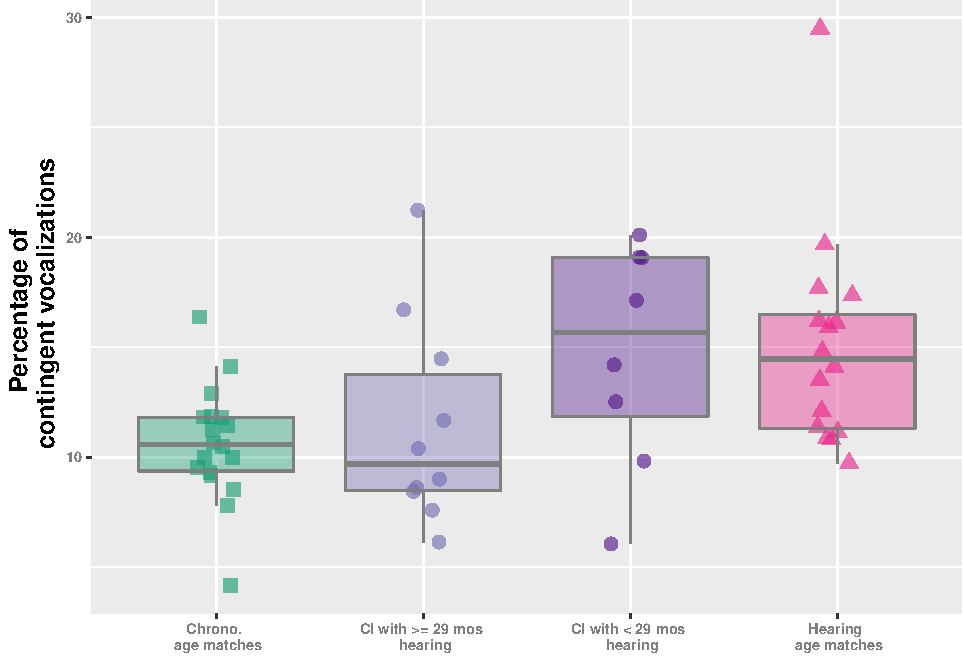
\includegraphics{everyday_CI_files/figure-latex/visualize perc contingent vocs by hearing group-1.pdf}

\begin{Shaded}
\begin{Highlighting}[]
\NormalTok{contingent\_final }\SpecialCharTok{\%\textgreater{}\%}
  \FunctionTok{mutate}\NormalTok{(}\AttributeTok{match=}\FunctionTok{recode}\NormalTok{(match,}
                      \AttributeTok{chrono=}\StringTok{\textquotesingle{}Chrono. }\SpecialCharTok{\textbackslash{}n}\StringTok{ age matches\textquotesingle{}}\NormalTok{,}
                      \AttributeTok{CI=}\StringTok{\textquotesingle{}CI by }\SpecialCharTok{\textbackslash{}n}\StringTok{ chrono. age\textquotesingle{}}\NormalTok{,}
                      \AttributeTok{CI\_by\_hearing\_age=}\StringTok{\textquotesingle{}CI by }\SpecialCharTok{\textbackslash{}n}\StringTok{ hearing age\textquotesingle{}}\NormalTok{,}
                      \AttributeTok{HA=}\StringTok{\textquotesingle{}Hearing }\SpecialCharTok{\textbackslash{}n}\StringTok{ age matches\textquotesingle{}}\NormalTok{)) }\SpecialCharTok{\%\textgreater{}\%}
\FunctionTok{ggplot}\NormalTok{(., }\FunctionTok{aes}\NormalTok{(age\_mos, perc\_contingent)) }\SpecialCharTok{+}
  \FunctionTok{geom\_jitter}\NormalTok{(}\FunctionTok{aes}\NormalTok{(}\AttributeTok{color=}\NormalTok{match, }\AttributeTok{fill=}\NormalTok{match, }\AttributeTok{shape=}\NormalTok{match),}\AttributeTok{size=}\FloatTok{2.8}\NormalTok{,}\AttributeTok{alpha=}\NormalTok{.}\DecValTok{6}\NormalTok{,}\AttributeTok{width =}\NormalTok{ .}\DecValTok{3}\NormalTok{) }\SpecialCharTok{+}
  \FunctionTok{geom\_smooth}\NormalTok{(}\FunctionTok{aes}\NormalTok{(}\AttributeTok{fill=}\NormalTok{match, }\AttributeTok{color=}\NormalTok{match), }\AttributeTok{method =} \StringTok{"lm"}\NormalTok{,}\AttributeTok{size=}\FloatTok{1.2}\NormalTok{) }\SpecialCharTok{+} 
  \FunctionTok{facet\_grid}\NormalTok{(}\SpecialCharTok{\textasciitilde{}}\NormalTok{match) }\SpecialCharTok{+}
  \FunctionTok{scale\_color\_brewer}\NormalTok{(}\AttributeTok{palette =} \StringTok{"Dark2"}\NormalTok{) }\SpecialCharTok{+}
  \FunctionTok{scale\_fill\_brewer}\NormalTok{(}\AttributeTok{palette =} \StringTok{"Dark2"}\NormalTok{) }\SpecialCharTok{+}
  \FunctionTok{scale\_shape\_manual}\NormalTok{(}\AttributeTok{values=}\FunctionTok{c}\NormalTok{(}\DecValTok{15}\NormalTok{,}\DecValTok{16}\NormalTok{,}\DecValTok{16}\NormalTok{,}\DecValTok{17}\NormalTok{)) }\SpecialCharTok{+}
  \FunctionTok{xlab}\NormalTok{(}\StringTok{"Age (mos)"}\NormalTok{) }\SpecialCharTok{+}
  \FunctionTok{ylab}\NormalTok{(}\StringTok{"Percentage of }\SpecialCharTok{\textbackslash{}n}\StringTok{ contingent vocalizations"}\NormalTok{) }\SpecialCharTok{+} 
    \FunctionTok{theme}\NormalTok{(}\AttributeTok{axis.title =} \FunctionTok{element\_text}\NormalTok{(}\AttributeTok{face =}\StringTok{"bold"}\NormalTok{, }\AttributeTok{size=}\DecValTok{12}\NormalTok{),}
        \AttributeTok{legend.position =} \StringTok{"none"}\NormalTok{, }
        \AttributeTok{axis.text =} \FunctionTok{element\_text}\NormalTok{(}\AttributeTok{face=}\StringTok{"bold"}\NormalTok{, }\AttributeTok{color=}\StringTok{\textquotesingle{}gray50\textquotesingle{}}\NormalTok{, }\AttributeTok{size=}\DecValTok{9}\NormalTok{),}
        \AttributeTok{strip.text=}\FunctionTok{element\_text}\NormalTok{(}\AttributeTok{face=}\StringTok{\textquotesingle{}bold\textquotesingle{}}\NormalTok{, }\AttributeTok{size=}\DecValTok{10}\NormalTok{))}
\end{Highlighting}
\end{Shaded}

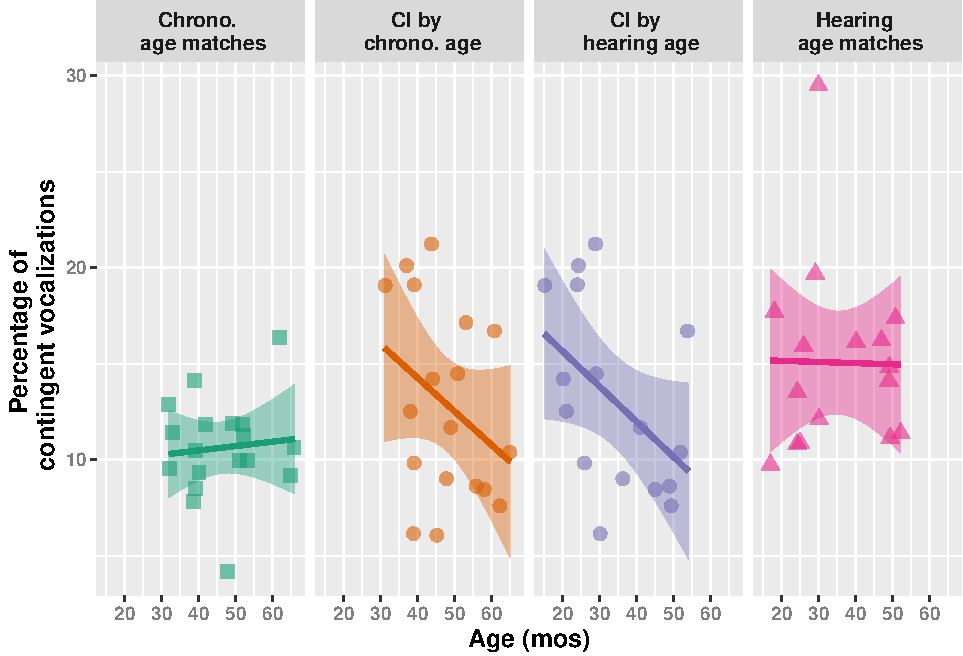
\includegraphics{everyday_CI_files/figure-latex/visualize perc contingent vocs by age-1.pdf}

\begin{Shaded}
\begin{Highlighting}[]
\CommentTok{\# are kids more likely to respond to louder speech? does this vary by hearing group?}
\NormalTok{intens2 }\SpecialCharTok{\%\textgreater{}\%}
    \FunctionTok{mutate}\NormalTok{(}\AttributeTok{match=}\FunctionTok{recode}\NormalTok{(match,}
                      \AttributeTok{chrono=}\StringTok{\textquotesingle{}Chrono. }\SpecialCharTok{\textbackslash{}n}\StringTok{ age matches\textquotesingle{}}\NormalTok{,}
                      \AttributeTok{CI=}\StringTok{\textquotesingle{}Cochlear implant\textquotesingle{}}\NormalTok{,}
                      \AttributeTok{HA=}\StringTok{\textquotesingle{}Hearing }\SpecialCharTok{\textbackslash{}n}\StringTok{ age matches\textquotesingle{}}\NormalTok{)) }\SpecialCharTok{\%\textgreater{}\%}
\FunctionTok{ggplot}\NormalTok{(., }\FunctionTok{aes}\NormalTok{(}\AttributeTok{x=}\NormalTok{adult\_loudness, }\AttributeTok{y=}\NormalTok{perc\_contingent\_loudness)) }\SpecialCharTok{+} 
    \FunctionTok{geom\_point}\NormalTok{(}\FunctionTok{aes}\NormalTok{(}\AttributeTok{fill=}\NormalTok{match,}\AttributeTok{shape=}\NormalTok{match,}\AttributeTok{group=}\NormalTok{child\_id,}\AttributeTok{color=}\NormalTok{match, }\AttributeTok{alpha=}\NormalTok{adult\_loudness),}
                \AttributeTok{size=}\FloatTok{2.5}\NormalTok{, }\AttributeTok{position=}\FunctionTok{position\_jitter}\NormalTok{(}\FloatTok{0.02}\NormalTok{)) }\SpecialCharTok{+} 
    \FunctionTok{geom\_line}\NormalTok{(}\FunctionTok{aes}\NormalTok{(}\AttributeTok{group =}\NormalTok{ child\_id), }\AttributeTok{color=}\StringTok{"gray50"}\NormalTok{,}\AttributeTok{size =}\NormalTok{ .}\DecValTok{45}\NormalTok{, }\AttributeTok{alpha =} \FloatTok{0.5}\NormalTok{) }\SpecialCharTok{+} 
    \FunctionTok{geom\_boxplot}\NormalTok{(}\FunctionTok{aes}\NormalTok{(}\AttributeTok{fill=}\NormalTok{match, }\AttributeTok{alpha=}\NormalTok{adult\_loudness),}\AttributeTok{notch=}\ConstantTok{FALSE}\NormalTok{,}\AttributeTok{size=}\NormalTok{.}\DecValTok{5}\NormalTok{, }\AttributeTok{outlier.shape =} \ConstantTok{NA}\NormalTok{,}
                 \AttributeTok{width=}\FloatTok{0.6}\NormalTok{,}\AttributeTok{color=}\StringTok{"gray50"}\NormalTok{, }\AttributeTok{position=}\FunctionTok{position\_dodge}\NormalTok{(.}\DecValTok{6}\NormalTok{),) }\SpecialCharTok{+}
    \FunctionTok{facet\_wrap}\NormalTok{(}\SpecialCharTok{\textasciitilde{}}\NormalTok{match) }\SpecialCharTok{+}
   \FunctionTok{scale\_fill\_manual}\NormalTok{(}\AttributeTok{values=}\FunctionTok{c}\NormalTok{(}\StringTok{"\#1B9E77"}\NormalTok{, }\StringTok{"\#7570B3"}\NormalTok{, }\StringTok{"\#E7298A"}\NormalTok{))}\SpecialCharTok{+}
   \FunctionTok{scale\_color\_manual}\NormalTok{(}\AttributeTok{values=}\FunctionTok{c}\NormalTok{(}\StringTok{"\#1B9E77"}\NormalTok{, }\StringTok{"\#7570B3"}\NormalTok{, }\StringTok{"\#E7298A"}\NormalTok{))}\SpecialCharTok{+}
     \FunctionTok{scale\_alpha\_manual}\NormalTok{(}\AttributeTok{values=}\FunctionTok{c}\NormalTok{(.}\DecValTok{3}\NormalTok{, .}\DecValTok{5}\NormalTok{))}\SpecialCharTok{+}
  \FunctionTok{scale\_shape\_manual}\NormalTok{(}\AttributeTok{values=}\FunctionTok{c}\NormalTok{(}\DecValTok{15}\NormalTok{,}\DecValTok{16}\NormalTok{,}\DecValTok{17}\NormalTok{)) }\SpecialCharTok{+}

  \FunctionTok{labs}\NormalTok{(}\AttributeTok{x=}\StringTok{"Intensity of caregiver speech"}\NormalTok{,}\AttributeTok{y=}\StringTok{"Percentage of all }\SpecialCharTok{\textbackslash{}n}\StringTok{ vocalizations that are contingent"}\NormalTok{) }\SpecialCharTok{+}
  \FunctionTok{guides}\NormalTok{(}\AttributeTok{alpha=}\StringTok{"none"}\NormalTok{, }\AttributeTok{fill =} \StringTok{"none"}\NormalTok{,}\AttributeTok{color=}\StringTok{"none"}\NormalTok{,}\AttributeTok{shape=}\StringTok{"none"}\NormalTok{) }\SpecialCharTok{+}
  \FunctionTok{theme}\NormalTok{(}\AttributeTok{legend.position =} \FunctionTok{c}\NormalTok{(.}\DecValTok{8}\NormalTok{, .}\DecValTok{8}\NormalTok{),}
        \AttributeTok{axis.ticks =} \FunctionTok{element\_blank}\NormalTok{(),}
        \AttributeTok{legend.title=}\FunctionTok{element\_text}\NormalTok{(}\AttributeTok{face=}\StringTok{"bold"}\NormalTok{, }\AttributeTok{size=}\DecValTok{13}\NormalTok{),}
        \AttributeTok{legend.text=}\FunctionTok{element\_text}\NormalTok{(}\AttributeTok{face=}\StringTok{"bold"}\NormalTok{, }\AttributeTok{size=}\DecValTok{9}\NormalTok{),}
        \AttributeTok{axis.text =} \FunctionTok{element\_text}\NormalTok{(}\AttributeTok{face =}\StringTok{\textquotesingle{}bold\textquotesingle{}}\NormalTok{, }\AttributeTok{size=}\DecValTok{12}\NormalTok{),}
        \AttributeTok{axis.title =} \FunctionTok{element\_text}\NormalTok{(}\AttributeTok{face =}\StringTok{\textquotesingle{}bold\textquotesingle{}}\NormalTok{, }\AttributeTok{size=}\DecValTok{16}\NormalTok{),}
        \AttributeTok{panel.grid.major.x =} \FunctionTok{element\_blank}\NormalTok{(),}
        \AttributeTok{strip.text.x =} \FunctionTok{element\_text}\NormalTok{(}\AttributeTok{face =} \StringTok{"bold"}\NormalTok{,}\AttributeTok{size=}\DecValTok{13}\NormalTok{),}
        \AttributeTok{strip.background =} \FunctionTok{element\_rect}\NormalTok{(}\AttributeTok{fill =} \StringTok{"gray60"}\NormalTok{, }\AttributeTok{size =} \DecValTok{1}\NormalTok{)) }
\end{Highlighting}
\end{Shaded}

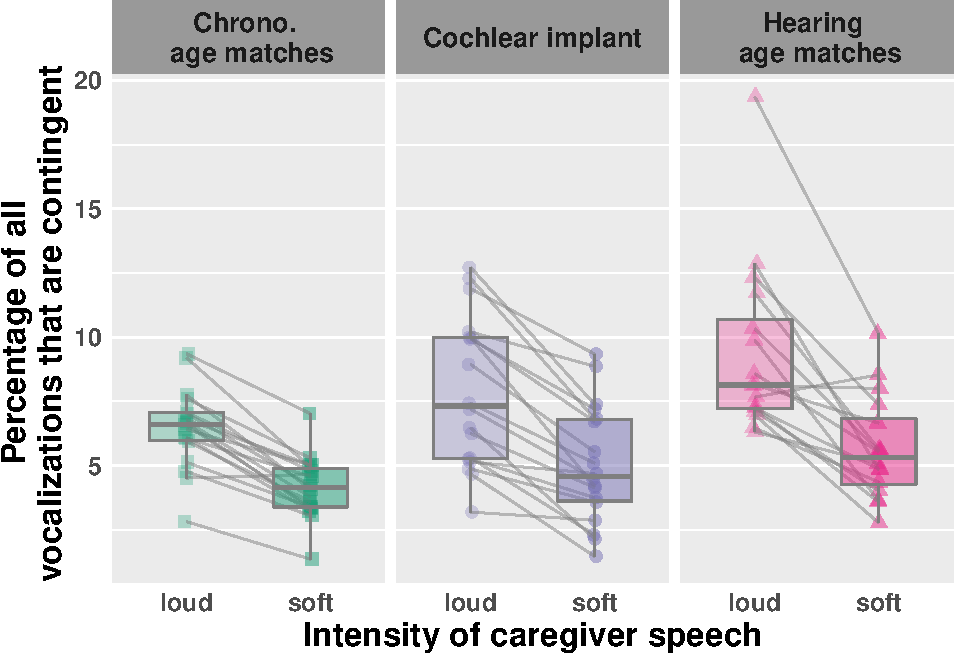
\includegraphics{everyday_CI_files/figure-latex/visualize split by intensity-1.pdf}

\begin{Shaded}
\begin{Highlighting}[]
\NormalTok{temp\_boxplot }\OtherTok{\textless{}{-}}\NormalTok{ time\_vocs\_final }\SpecialCharTok{\%\textgreater{}\%} 
  \FunctionTok{filter}\NormalTok{(match}\SpecialCharTok{==}\StringTok{\textquotesingle{}CI\textquotesingle{}}\NormalTok{) }\SpecialCharTok{\%\textgreater{}\%}
  \FunctionTok{mutate}\NormalTok{(}\AttributeTok{med\_hearing\_age =} \FunctionTok{median}\NormalTok{(hearing\_age)) }\SpecialCharTok{\%\textgreater{}\%}
  \FunctionTok{mutate}\NormalTok{(}\AttributeTok{match=}\FunctionTok{if\_else}\NormalTok{(hearing\_age }\SpecialCharTok{\textgreater{}=}\NormalTok{ med\_hearing\_age, }\StringTok{\textquotesingle{}more\textquotesingle{}}\NormalTok{, }\StringTok{\textquotesingle{}less\textquotesingle{}}\NormalTok{)) }\SpecialCharTok{\%\textgreater{}\%}
  \FunctionTok{select}\NormalTok{(}\SpecialCharTok{{-}}\NormalTok{med\_hearing\_age)}

\NormalTok{temp\_boxplot2 }\OtherTok{\textless{}{-}}\NormalTok{ time\_vocs\_final }\SpecialCharTok{\%\textgreater{}\%}
  \FunctionTok{filter}\NormalTok{(match}\SpecialCharTok{==}\StringTok{\textquotesingle{}HA\textquotesingle{}} \SpecialCharTok{|}\NormalTok{ match}\SpecialCharTok{==}\StringTok{\textquotesingle{}chrono\textquotesingle{}}\NormalTok{) }\SpecialCharTok{\%\textgreater{}\%}
  \FunctionTok{rbind}\NormalTok{(., temp\_boxplot)}

\NormalTok{temp\_boxplot2 }\SpecialCharTok{\%\textgreater{}\%}
  \FunctionTok{mutate}\NormalTok{(}\AttributeTok{match=}\FunctionTok{factor}\NormalTok{(match, }\AttributeTok{levels =} \FunctionTok{c}\NormalTok{(}\StringTok{"chrono"}\NormalTok{, }\StringTok{"more"}\NormalTok{, }\StringTok{"less"}\NormalTok{, }\StringTok{"HA"}\NormalTok{))) }\SpecialCharTok{\%\textgreater{}\%}
   \FunctionTok{mutate}\NormalTok{(}\AttributeTok{match=}\FunctionTok{recode}\NormalTok{(match,}
                      \AttributeTok{chrono=}\StringTok{\textquotesingle{}Chrono. }\SpecialCharTok{\textbackslash{}n}\StringTok{ age matches\textquotesingle{}}\NormalTok{,}
                      \AttributeTok{more=}\StringTok{\textquotesingle{}CI with \textgreater{}= 29 mos }\SpecialCharTok{\textbackslash{}n}\StringTok{ hearing\textquotesingle{}}\NormalTok{,}
                      \AttributeTok{less=}\StringTok{\textquotesingle{}CI with \textless{} 29 mos }\SpecialCharTok{\textbackslash{}n}\StringTok{ hearing\textquotesingle{}}\NormalTok{,}
                      \AttributeTok{HA=}\StringTok{\textquotesingle{}Hearing }\SpecialCharTok{\textbackslash{}n}\StringTok{ age matches\textquotesingle{}}\NormalTok{)) }\SpecialCharTok{\%\textgreater{}\%}
   \CommentTok{\#group\_by(match,child\_id) \%\textgreater{}\%}
   \CommentTok{\#summarize(mean\_speech\_lag=mean(speech\_lag*1000)) \%\textgreater{}\%}
\FunctionTok{ggplot}\NormalTok{(., }\FunctionTok{aes}\NormalTok{(match, speech\_lag)) }\SpecialCharTok{+}
  \FunctionTok{geom\_jitter}\NormalTok{(}\FunctionTok{aes}\NormalTok{(}\AttributeTok{color=}\NormalTok{match, }\AttributeTok{fill=}\NormalTok{match,}\AttributeTok{shape=}\NormalTok{match),}\AttributeTok{size=}\FloatTok{2.8}\NormalTok{,}\AttributeTok{width =}\NormalTok{ .}\DecValTok{1}\NormalTok{,}\AttributeTok{alpha=}\NormalTok{.}\DecValTok{65}\NormalTok{) }\SpecialCharTok{+}
  \FunctionTok{geom\_boxplot}\NormalTok{(}\FunctionTok{aes}\NormalTok{(}\AttributeTok{fill=}\NormalTok{match), }\AttributeTok{alpha=}\NormalTok{.}\DecValTok{4}\NormalTok{, }\AttributeTok{color=}\StringTok{\textquotesingle{}gray50\textquotesingle{}}\NormalTok{, }\AttributeTok{outlier.shape =} \ConstantTok{NA}\NormalTok{) }\SpecialCharTok{+}
  \FunctionTok{scale\_color\_manual}\NormalTok{(}\AttributeTok{values=}\FunctionTok{c}\NormalTok{(}\StringTok{"\#1B9E77"}\NormalTok{, }\StringTok{"\#7570B3"}\NormalTok{, }\StringTok{"purple4"}\NormalTok{, }\StringTok{"\#E7298A"}\NormalTok{))}\SpecialCharTok{+}
  \FunctionTok{scale\_fill\_manual}\NormalTok{(}\AttributeTok{values=}\FunctionTok{c}\NormalTok{(}\StringTok{"\#1B9E77"}\NormalTok{, }\StringTok{"\#7570B3"}\NormalTok{, }\StringTok{"purple4"}\NormalTok{, }\StringTok{"\#E7298A"}\NormalTok{)) }\SpecialCharTok{+}
  \FunctionTok{scale\_shape\_manual}\NormalTok{(}\AttributeTok{values=}\FunctionTok{c}\NormalTok{(}\DecValTok{15}\NormalTok{,}\DecValTok{16}\NormalTok{,}\DecValTok{16}\NormalTok{,}\DecValTok{17}\NormalTok{)) }\SpecialCharTok{+}
  \FunctionTok{ylab}\NormalTok{(}\StringTok{"Avg. temporal lag between }\SpecialCharTok{\textbackslash{}n}\StringTok{ adult and child vocalizations (ms)"}\NormalTok{) }\SpecialCharTok{+} 
  \CommentTok{\#ggtitle("Contingent vocalizations, by hearing group") + }
  \FunctionTok{theme}\NormalTok{(}\AttributeTok{legend.position =} \StringTok{"none"}\NormalTok{,}
        \AttributeTok{axis.title.y =} \FunctionTok{element\_text}\NormalTok{(}\AttributeTok{face =}\StringTok{"bold"}\NormalTok{, }\AttributeTok{size=}\DecValTok{12}\NormalTok{),}
        \AttributeTok{axis.title.x =} \FunctionTok{element\_blank}\NormalTok{(),}
        \AttributeTok{axis.text.y =} \FunctionTok{element\_text}\NormalTok{(}\AttributeTok{face=}\StringTok{"bold"}\NormalTok{, }\AttributeTok{color=}\StringTok{\textquotesingle{}gray50\textquotesingle{}}\NormalTok{, }\AttributeTok{size=}\DecValTok{7}\NormalTok{),}
        \AttributeTok{axis.text.x =} \FunctionTok{element\_text}\NormalTok{(}\AttributeTok{face=}\StringTok{"bold"}\NormalTok{, }\AttributeTok{color=}\StringTok{\textquotesingle{}gray50\textquotesingle{}}\NormalTok{, }\AttributeTok{size=}\DecValTok{10}\NormalTok{),}
        \AttributeTok{plot.title =} \FunctionTok{element\_text}\NormalTok{(}\AttributeTok{face=}\StringTok{"bold"}\NormalTok{, }\AttributeTok{size=}\DecValTok{16}\NormalTok{))}
\end{Highlighting}
\end{Shaded}

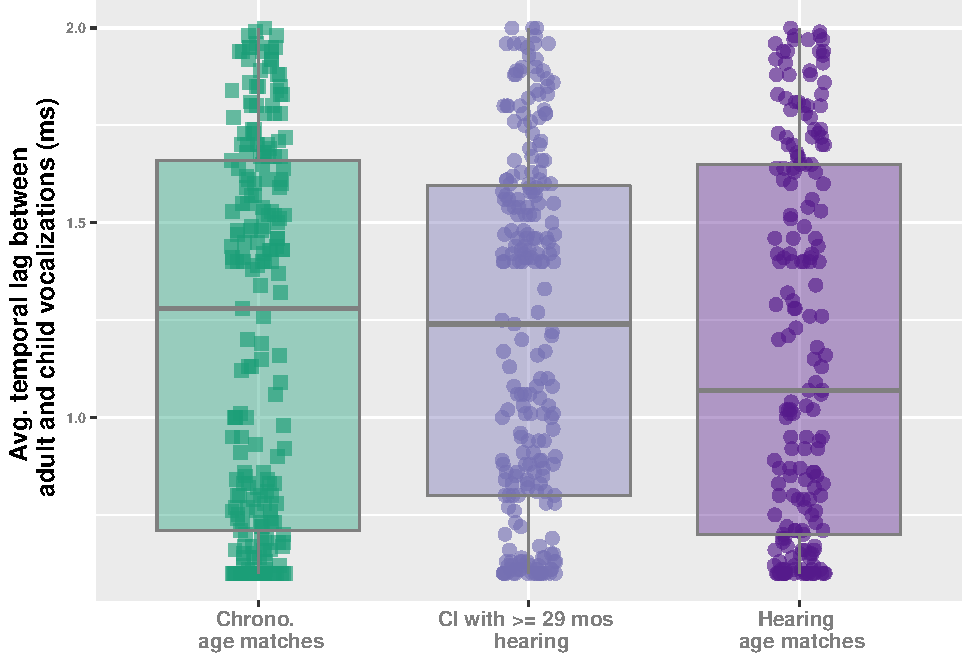
\includegraphics{everyday_CI_files/figure-latex/visualize temporal dyanmics by hearing group-1.pdf}

\hypertarget{model-contingency}{%
\subsection{Model contingency}\label{model-contingency}}

\begin{Shaded}
\begin{Highlighting}[]
\CommentTok{\# {-}{-}{-}{-}{-}{-}{-} look at percentage contingent {-}{-}{-}{-}{-}{-}{-}}
\CommentTok{\# look at just three groups}
\NormalTok{contingent\_final\_3 }\OtherTok{\textless{}{-}}\NormalTok{ contingent\_final }\SpecialCharTok{\%\textgreater{}\%} \FunctionTok{filter}\NormalTok{(match}\SpecialCharTok{!=}\StringTok{\textquotesingle{}CI\_by\_hearing\_age\textquotesingle{}}\NormalTok{)}
\NormalTok{contingent\_final\_3}\SpecialCharTok{$}\NormalTok{match }\OtherTok{\textless{}{-}} \FunctionTok{relevel}\NormalTok{(}\FunctionTok{factor}\NormalTok{(contingent\_final\_3}\SpecialCharTok{$}\NormalTok{match), }\AttributeTok{ref =} \StringTok{"chrono"}\NormalTok{)}
\NormalTok{m1 }\OtherTok{\textless{}{-}} \FunctionTok{lm}\NormalTok{(perc\_contingent}\SpecialCharTok{\textasciitilde{}}\NormalTok{match, }\AttributeTok{data=}\NormalTok{contingent\_final\_3)}
\FunctionTok{summary}\NormalTok{(m1)}
\end{Highlighting}
\end{Shaded}

\begin{verbatim}
## 
## Call:
## lm(formula = perc_contingent ~ match, data = contingent_final_3)
## 
## Residuals:
##     Min      1Q  Median      3Q     Max 
## -6.8452 -2.9846 -0.3205  1.7434 14.4340 
## 
## Coefficients:
##             Estimate Std. Error t value Pr(>|t|)    
## (Intercept)   10.622      1.005  10.566 3.13e-14 ***
## matchCI        2.283      1.422   1.606  0.11479    
## matchHA        4.434      1.465   3.025  0.00395 ** 
## ---
## Signif. codes:  0 '***' 0.001 '**' 0.01 '*' 0.05 '.' 0.1 ' ' 1
## 
## Residual standard error: 4.265 on 49 degrees of freedom
## Multiple R-squared:  0.1578, Adjusted R-squared:  0.1234 
## F-statistic: 4.589 on 2 and 49 DF,  p-value: 0.0149
\end{verbatim}

\begin{Shaded}
\begin{Highlighting}[]
\CommentTok{\# what\textquotesingle{}s the correlation between age and perc contingent for kids with CIs?}
\NormalTok{ci\_for\_cor }\OtherTok{\textless{}{-}}\NormalTok{ contingent\_final\_3 }\SpecialCharTok{\%\textgreater{}\%} \FunctionTok{filter}\NormalTok{(match}\SpecialCharTok{==}\StringTok{\textquotesingle{}CI\textquotesingle{}}\NormalTok{)}
\NormalTok{ci\_cor }\OtherTok{\textless{}{-}} \FunctionTok{cor.test}\NormalTok{(ci\_for\_cor}\SpecialCharTok{$}\NormalTok{age\_mos, ci\_for\_cor}\SpecialCharTok{$}\NormalTok{perc\_contingent)}
\NormalTok{ci\_cor\_aoi }\OtherTok{\textless{}{-}} \FunctionTok{cor.test}\NormalTok{(ci\_for\_cor}\SpecialCharTok{$}\NormalTok{age\_of\_implantation, ci\_for\_cor}\SpecialCharTok{$}\NormalTok{perc\_contingent)}

\CommentTok{\# look at HA, chrono, and more vs. less hearing experience groups}
\NormalTok{cont\_boxplot2}\SpecialCharTok{$}\NormalTok{match }\OtherTok{\textless{}{-}} \FunctionTok{relevel}\NormalTok{(}\FunctionTok{factor}\NormalTok{(cont\_boxplot2}\SpecialCharTok{$}\NormalTok{match), }\AttributeTok{ref =} \StringTok{"HA"}\NormalTok{)}
\NormalTok{ha\_model }\OtherTok{\textless{}{-}} \FunctionTok{lm}\NormalTok{(perc\_contingent}\SpecialCharTok{\textasciitilde{}}\NormalTok{match, }\AttributeTok{data=}\NormalTok{cont\_boxplot2)}
\FunctionTok{summary}\NormalTok{(ha\_model) }\CommentTok{\# the kids with more experience differ from the hearing age matches, as expected}
\end{Highlighting}
\end{Shaded}

\begin{verbatim}
## 
## Call:
## lm(formula = perc_contingent ~ match, data = cont_boxplot2)
## 
## Residuals:
##     Min      1Q  Median      3Q     Max 
## -8.6923 -2.8033 -0.4043  2.2772 14.4340 
## 
## Coefficients:
##             Estimate Std. Error t value Pr(>|t|)    
## (Intercept)  15.0559     1.0472  14.377  < 2e-16 ***
## matchchrono  -4.4337     1.4393  -3.081  0.00342 ** 
## matchless    -0.3039     1.8138  -0.168  0.86766    
## matchmore    -3.6287     1.6886  -2.149  0.03671 *  
## ---
## Signif. codes:  0 '***' 0.001 '**' 0.01 '*' 0.05 '.' 0.1 ' ' 1
## 
## Residual standard error: 4.189 on 48 degrees of freedom
## Multiple R-squared:  0.2042, Adjusted R-squared:  0.1544 
## F-statistic: 4.105 on 3 and 48 DF,  p-value: 0.01133
\end{verbatim}

\begin{Shaded}
\begin{Highlighting}[]
\NormalTok{cont\_boxplot2}\SpecialCharTok{$}\NormalTok{match }\OtherTok{\textless{}{-}} \FunctionTok{relevel}\NormalTok{(}\FunctionTok{factor}\NormalTok{(cont\_boxplot2}\SpecialCharTok{$}\NormalTok{match), }\AttributeTok{ref =} \StringTok{"chrono"}\NormalTok{)}
\NormalTok{chrono\_model }\OtherTok{\textless{}{-}} \FunctionTok{lm}\NormalTok{(perc\_contingent}\SpecialCharTok{\textasciitilde{}}\NormalTok{match, }\AttributeTok{data=}\NormalTok{cont\_boxplot2)}
\FunctionTok{summary}\NormalTok{(chrono\_model) }\CommentTok{\# the kids with less experience differ from the chrono age matches, as expected}
\end{Highlighting}
\end{Shaded}

\begin{verbatim}
## 
## Call:
## lm(formula = perc_contingent ~ match, data = cont_boxplot2)
## 
## Residuals:
##     Min      1Q  Median      3Q     Max 
## -8.6923 -2.8033 -0.4043  2.2772 14.4340 
## 
## Coefficients:
##             Estimate Std. Error t value Pr(>|t|)    
## (Intercept)  10.6222     0.9873  10.758 2.19e-14 ***
## matchHA       4.4337     1.4393   3.081  0.00342 ** 
## matchless     4.1298     1.7799   2.320  0.02463 *  
## matchmore     0.8050     1.6521   0.487  0.62830    
## ---
## Signif. codes:  0 '***' 0.001 '**' 0.01 '*' 0.05 '.' 0.1 ' ' 1
## 
## Residual standard error: 4.189 on 48 degrees of freedom
## Multiple R-squared:  0.2042, Adjusted R-squared:  0.1544 
## F-statistic: 4.105 on 3 and 48 DF,  p-value: 0.01133
\end{verbatim}

\begin{Shaded}
\begin{Highlighting}[]
\NormalTok{cont\_m0 }\OtherTok{\textless{}{-}} \FunctionTok{lm}\NormalTok{(perc\_contingent}\SpecialCharTok{\textasciitilde{}}\NormalTok{age\_mos, }\AttributeTok{data=}\NormalTok{contingent\_final\_3) }
\NormalTok{cont\_m1 }\OtherTok{\textless{}{-}} \FunctionTok{lm}\NormalTok{(perc\_contingent}\SpecialCharTok{\textasciitilde{}}\NormalTok{age\_mos }\SpecialCharTok{+}\NormalTok{ match, }\AttributeTok{data=}\NormalTok{contingent\_final\_3) }
\NormalTok{cont\_m2 }\OtherTok{\textless{}{-}} \FunctionTok{lm}\NormalTok{(perc\_contingent}\SpecialCharTok{\textasciitilde{}}\NormalTok{age\_mos}\SpecialCharTok{*}\NormalTok{match, }\AttributeTok{data=}\NormalTok{contingent\_final\_3) }

\FunctionTok{anova}\NormalTok{(cont\_m0, cont\_m1)}
\end{Highlighting}
\end{Shaded}

\begin{verbatim}
## Analysis of Variance Table
## 
## Model 1: perc_contingent ~ age_mos
## Model 2: perc_contingent ~ age_mos + match
##   Res.Df     RSS Df Sum of Sq      F  Pr(>F)  
## 1     50 1000.73                              
## 2     48  880.49  2    120.23 3.2773 0.04633 *
## ---
## Signif. codes:  0 '***' 0.001 '**' 0.01 '*' 0.05 '.' 0.1 ' ' 1
\end{verbatim}

\begin{Shaded}
\begin{Highlighting}[]
\FunctionTok{anova}\NormalTok{(cont\_m1, cont\_m2)}
\end{Highlighting}
\end{Shaded}

\begin{verbatim}
## Analysis of Variance Table
## 
## Model 1: perc_contingent ~ age_mos + match
## Model 2: perc_contingent ~ age_mos * match
##   Res.Df    RSS Df Sum of Sq      F Pr(>F)
## 1     48 880.49                           
## 2     46 840.10  2    40.394 1.1059 0.3396
\end{verbatim}

\begin{Shaded}
\begin{Highlighting}[]
\CommentTok{\# {-}{-}{-}{-}{-}{-} look at temporal dynamics {-}{-}{-}{-}{-}{-}{-}}
\CommentTok{\# for all kids?}
\NormalTok{time\_vocs\_final2 }\OtherTok{\textless{}{-}}\NormalTok{ time\_vocs\_final }\SpecialCharTok{\%\textgreater{}\%} \FunctionTok{filter}\NormalTok{(match}\SpecialCharTok{!=}\StringTok{\textquotesingle{}chrono\textquotesingle{}}\NormalTok{)}
\NormalTok{time\_vocs\_final2}\SpecialCharTok{$}\NormalTok{match }\OtherTok{\textless{}{-}} \FunctionTok{relevel}\NormalTok{(}\FunctionTok{factor}\NormalTok{(time\_vocs\_final2}\SpecialCharTok{$}\NormalTok{match), }\AttributeTok{ref =} \StringTok{"CI"}\NormalTok{)}
\NormalTok{m0\_lag }\OtherTok{\textless{}{-}} \FunctionTok{lmer}\NormalTok{(speech\_lag}\SpecialCharTok{*}\DecValTok{1000}\SpecialCharTok{\textasciitilde{}}\NormalTok{match }\SpecialCharTok{+}\NormalTok{ (}\DecValTok{1} \SpecialCharTok{|}\NormalTok{ child\_id), }\AttributeTok{data=}\NormalTok{time\_vocs\_final2)}
\NormalTok{m1\_lag }\OtherTok{\textless{}{-}} \FunctionTok{lmer}\NormalTok{(speech\_lag}\SpecialCharTok{*}\DecValTok{1000}\SpecialCharTok{\textasciitilde{}}\NormalTok{ match}\SpecialCharTok{+}\NormalTok{age\_mos}\SpecialCharTok{+}\NormalTok{(}\DecValTok{1}\SpecialCharTok{|}\NormalTok{child\_id), }\AttributeTok{data=}\NormalTok{time\_vocs\_final2)}
\FunctionTok{anova}\NormalTok{(m0\_lag,m1\_lag) }\CommentTok{\# no improvement }
\end{Highlighting}
\end{Shaded}

\begin{verbatim}
## Data: time_vocs_final2
## Models:
## m0_lag: speech_lag * 1000 ~ match + (1 | child_id)
## m1_lag: speech_lag * 1000 ~ match + age_mos + (1 | child_id)
##        npar    AIC    BIC  logLik deviance Chisq Df Pr(>Chisq)
## m0_lag    5 9434.7 9456.9 -4712.4   9424.7                    
## m1_lag    6 9436.4 9463.1 -4712.2   9424.4 0.298  1     0.5851
\end{verbatim}

\begin{Shaded}
\begin{Highlighting}[]
\NormalTok{m2\_lag }\OtherTok{\textless{}{-}} \FunctionTok{lmer}\NormalTok{(speech\_lag}\SpecialCharTok{*}\DecValTok{1000}\SpecialCharTok{\textasciitilde{}}\NormalTok{ match}\SpecialCharTok{*}\NormalTok{age\_mos}\SpecialCharTok{+}\NormalTok{(}\DecValTok{1}\SpecialCharTok{|}\NormalTok{child\_id), }\AttributeTok{data=}\NormalTok{time\_vocs\_final2)}
\FunctionTok{anova}\NormalTok{(m1\_lag,m2\_lag) }\CommentTok{\# no improvement }
\end{Highlighting}
\end{Shaded}

\begin{verbatim}
## Data: time_vocs_final2
## Models:
## m1_lag: speech_lag * 1000 ~ match + age_mos + (1 | child_id)
## m2_lag: speech_lag * 1000 ~ match * age_mos + (1 | child_id)
##        npar    AIC    BIC  logLik deviance Chisq Df Pr(>Chisq)
## m1_lag    6 9436.4 9463.1 -4712.2   9424.4                    
## m2_lag    8 9439.8 9475.3 -4711.9   9423.8 0.624  2      0.732
\end{verbatim}

\begin{Shaded}
\begin{Highlighting}[]
\CommentTok{\# what\textquotesingle{}s the association between age and temporal synchrony for kids with CIs?}
\NormalTok{ci\_temp\_for\_model }\OtherTok{\textless{}{-}}\NormalTok{ time\_vocs\_final }\SpecialCharTok{\%\textgreater{}\%} \FunctionTok{filter}\NormalTok{(match}\SpecialCharTok{==}\StringTok{\textquotesingle{}CI\textquotesingle{}}\NormalTok{)}
\NormalTok{ci\_temp\_m }\OtherTok{\textless{}{-}} \FunctionTok{lmer}\NormalTok{(speech\_lag}\SpecialCharTok{*}\DecValTok{1000}\SpecialCharTok{\textasciitilde{}}\NormalTok{hearing\_age }\SpecialCharTok{+}\NormalTok{ (}\DecValTok{1}\SpecialCharTok{|}\NormalTok{child\_id), }\AttributeTok{data=}\NormalTok{ci\_temp\_for\_model)}
\FunctionTok{summary}\NormalTok{(ci\_temp\_m)}
\end{Highlighting}
\end{Shaded}

\begin{verbatim}
## Linear mixed model fit by REML. t-tests use Satterthwaite's method [
## lmerModLmerTest]
## Formula: speech_lag * 1000 ~ hearing_age + (1 | child_id)
##    Data: ci_temp_for_model
## 
## REML criterion at convergence: 3470.4
## 
## Scaled residuals: 
##      Min       1Q   Median       3Q      Max 
## -1.40200 -0.90924  0.01766  0.81871  1.71995 
## 
## Random effects:
##  Groups   Name        Variance Std.Dev.
##  child_id (Intercept)   1418    37.66  
##  Residual             206984   454.95  
## Number of obs: 231, groups:  child_id, 18
## 
## Fixed effects:
##              Estimate Std. Error        df t value Pr(>|t|)    
## (Intercept) 1225.0001    76.0482   14.3570  16.108 1.36e-10 ***
## hearing_age   -0.1716     2.2176   14.3767  -0.077    0.939    
## ---
## Signif. codes:  0 '***' 0.001 '**' 0.01 '*' 0.05 '.' 0.1 ' ' 1
## 
## Correlation of Fixed Effects:
##             (Intr)
## hearing_age -0.912
\end{verbatim}

\begin{Shaded}
\begin{Highlighting}[]
\CommentTok{\# look at HA, chrono, and more vs. less hearing experience groups for temporal synchrony}
\NormalTok{temp\_boxplot2}\SpecialCharTok{$}\NormalTok{match }\OtherTok{\textless{}{-}} \FunctionTok{relevel}\NormalTok{(}\FunctionTok{factor}\NormalTok{(temp\_boxplot2}\SpecialCharTok{$}\NormalTok{match), }\AttributeTok{ref =} \StringTok{"HA"}\NormalTok{)}
\NormalTok{ha\_temp\_model }\OtherTok{\textless{}{-}} \FunctionTok{lmer}\NormalTok{(speech\_lag}\SpecialCharTok{*}\DecValTok{1000}\SpecialCharTok{\textasciitilde{}}\NormalTok{match}\SpecialCharTok{+}\NormalTok{(}\DecValTok{1}\SpecialCharTok{|}\NormalTok{child\_id), }\AttributeTok{data=}\NormalTok{temp\_boxplot2)}
\FunctionTok{summary}\NormalTok{(ha\_temp\_model) }\CommentTok{\# the kids with more experience differ from the hearing age matches, as expected}
\end{Highlighting}
\end{Shaded}

\begin{verbatim}
## Linear mixed model fit by REML. t-tests use Satterthwaite's method [
## lmerModLmerTest]
## Formula: speech_lag * 1000 ~ match + (1 | child_id)
##    Data: temp_boxplot2
## 
## REML criterion at convergence: 9687.8
## 
## Scaled residuals: 
##      Min       1Q   Median       3Q      Max 
## -1.30862 -1.00017 -0.02111  0.89944  1.72260 
## 
## Random effects:
##  Groups   Name        Variance Std.Dev.
##  child_id (Intercept)      0     0.0   
##  Residual             224470   473.8   
## Number of obs: 641, groups:  child_id, 52
## 
## Fixed effects:
##             Estimate Std. Error      df t value Pr(>|t|)    
## (Intercept)  1183.86      34.46  638.00  34.352   <2e-16 ***
## matchchrono    23.42      46.94  638.00   0.499    0.618    
## matchmore      36.14      46.47  638.00   0.778    0.437    
## ---
## Signif. codes:  0 '***' 0.001 '**' 0.01 '*' 0.05 '.' 0.1 ' ' 1
## 
## Correlation of Fixed Effects:
##             (Intr) mtchch
## matchchrono -0.734       
## matchmore   -0.742  0.544
## optimizer (nloptwrap) convergence code: 0 (OK)
## boundary (singular) fit: see help('isSingular')
\end{verbatim}

\begin{Shaded}
\begin{Highlighting}[]
\NormalTok{temp\_boxplot2}\SpecialCharTok{$}\NormalTok{match }\OtherTok{\textless{}{-}} \FunctionTok{relevel}\NormalTok{(}\FunctionTok{factor}\NormalTok{(temp\_boxplot2}\SpecialCharTok{$}\NormalTok{match), }\AttributeTok{ref =} \StringTok{"chrono"}\NormalTok{)}
\NormalTok{chrono\_temp\_model }\OtherTok{\textless{}{-}} \FunctionTok{lmer}\NormalTok{(speech\_lag}\SpecialCharTok{*}\DecValTok{1000}\SpecialCharTok{\textasciitilde{}}\NormalTok{match}\SpecialCharTok{+}\NormalTok{(}\DecValTok{1}\SpecialCharTok{|}\NormalTok{child\_id), }\AttributeTok{data=}\NormalTok{temp\_boxplot2)}
\FunctionTok{summary}\NormalTok{(chrono\_temp\_model) }\CommentTok{\# the kids with less experience differ from the chrono age matches, as expected}
\end{Highlighting}
\end{Shaded}

\begin{verbatim}
## Linear mixed model fit by REML. t-tests use Satterthwaite's method [
## lmerModLmerTest]
## Formula: speech_lag * 1000 ~ match + (1 | child_id)
##    Data: temp_boxplot2
## 
## REML criterion at convergence: 9687.8
## 
## Scaled residuals: 
##      Min       1Q   Median       3Q      Max 
## -1.30862 -1.00017 -0.02111  0.89944  1.72260 
## 
## Random effects:
##  Groups   Name        Variance Std.Dev.
##  child_id (Intercept)      0     0.0   
##  Residual             224470   473.8   
## Number of obs: 641, groups:  child_id, 52
## 
## Fixed effects:
##             Estimate Std. Error      df t value Pr(>|t|)    
## (Intercept)  1207.29      31.87  638.00  37.881   <2e-16 ***
## matchHA       -23.42      46.94  638.00  -0.499    0.618    
## matchmore      12.71      44.58  638.00   0.285    0.776    
## ---
## Signif. codes:  0 '***' 0.001 '**' 0.01 '*' 0.05 '.' 0.1 ' ' 1
## 
## Correlation of Fixed Effects:
##           (Intr) mtchHA
## matchHA   -0.679       
## matchmore -0.715  0.485
## optimizer (nloptwrap) convergence code: 0 (OK)
## boundary (singular) fit: see help('isSingular')
\end{verbatim}

\begin{Shaded}
\begin{Highlighting}[]
\NormalTok{center\_scale }\OtherTok{\textless{}{-}} \ControlFlowTok{function}\NormalTok{(x) \{}
    \FunctionTok{scale}\NormalTok{(x, }\AttributeTok{scale =} \ConstantTok{FALSE}\NormalTok{)}
\NormalTok{\}}
\NormalTok{all\_intens\_vocs }\OtherTok{\textless{}{-}}\NormalTok{ all\_intens\_vocs }\SpecialCharTok{\%\textgreater{}\%}
  \FunctionTok{mutate}\NormalTok{(}\AttributeTok{adult\_voc\_dB\_centered =} \FunctionTok{center\_scale}\NormalTok{(adult\_voc\_dB)) }

\CommentTok{\#not using these}
\NormalTok{intens2}\SpecialCharTok{$}\NormalTok{match }\OtherTok{\textless{}{-}} \FunctionTok{relevel}\NormalTok{(}\FunctionTok{factor}\NormalTok{(intens2}\SpecialCharTok{$}\NormalTok{match), }\AttributeTok{ref =} \StringTok{"CI"}\NormalTok{)}
\NormalTok{intens\_m0 }\OtherTok{\textless{}{-}} \FunctionTok{lm}\NormalTok{(perc\_contingent\_loudness}\SpecialCharTok{\textasciitilde{}}\NormalTok{adult\_loudness, }\AttributeTok{data=}\NormalTok{intens2)}
\NormalTok{intens\_m1 }\OtherTok{\textless{}{-}} \FunctionTok{lm}\NormalTok{(perc\_contingent\_loudness}\SpecialCharTok{\textasciitilde{}}\NormalTok{match}\SpecialCharTok{+}\NormalTok{adult\_loudness, }\AttributeTok{data=}\NormalTok{intens2)}
\FunctionTok{anova}\NormalTok{(intens\_m0,intens\_m1)}
\end{Highlighting}
\end{Shaded}

\begin{verbatim}
## Analysis of Variance Table
## 
## Model 1: perc_contingent_loudness ~ adult_loudness
## Model 2: perc_contingent_loudness ~ match + adult_loudness
##   Res.Df    RSS Df Sum of Sq      F    Pr(>F)    
## 1    102 625.64                                  
## 2    100 542.15  2    83.483 7.6992 0.0007762 ***
## ---
## Signif. codes:  0 '***' 0.001 '**' 0.01 '*' 0.05 '.' 0.1 ' ' 1
\end{verbatim}

\begin{Shaded}
\begin{Highlighting}[]
\NormalTok{intens\_m2 }\OtherTok{\textless{}{-}} \FunctionTok{lm}\NormalTok{(perc\_contingent\_loudness}\SpecialCharTok{\textasciitilde{}}\NormalTok{match}\SpecialCharTok{*}\NormalTok{adult\_loudness, }\AttributeTok{data=}\NormalTok{intens2)}
\FunctionTok{anova}\NormalTok{(intens\_m1,intens\_m2) }\CommentTok{\# no interaction}
\end{Highlighting}
\end{Shaded}

\begin{verbatim}
## Analysis of Variance Table
## 
## Model 1: perc_contingent_loudness ~ match + adult_loudness
## Model 2: perc_contingent_loudness ~ match * adult_loudness
##   Res.Df    RSS Df Sum of Sq      F Pr(>F)
## 1    100 542.15                           
## 2     98 533.51  2    8.6462 0.7941 0.4549
\end{verbatim}

\begin{Shaded}
\begin{Highlighting}[]
\CommentTok{\# repeated measures model:}
\CommentTok{\# hearing status?}
\NormalTok{all\_intens\_vocs}\SpecialCharTok{$}\NormalTok{match }\OtherTok{\textless{}{-}} \FunctionTok{relevel}\NormalTok{(}\FunctionTok{factor}\NormalTok{(all\_intens\_vocs}\SpecialCharTok{$}\NormalTok{match), }\AttributeTok{ref =} \StringTok{"CI"}\NormalTok{)}
\NormalTok{lag\_m0 }\OtherTok{\textless{}{-}} \FunctionTok{lmer}\NormalTok{(speech\_lag}\SpecialCharTok{*}\DecValTok{1000}\SpecialCharTok{\textasciitilde{}} \SpecialCharTok{+}\NormalTok{ (}\DecValTok{1} \SpecialCharTok{|}\NormalTok{ child\_id), }\AttributeTok{data=}\NormalTok{all\_intens\_vocs)}
\NormalTok{lag\_m1 }\OtherTok{\textless{}{-}} \FunctionTok{lmer}\NormalTok{(speech\_lag}\SpecialCharTok{*}\DecValTok{1000}\SpecialCharTok{\textasciitilde{}}\NormalTok{ match }\SpecialCharTok{+}\NormalTok{ (}\DecValTok{1} \SpecialCharTok{|}\NormalTok{ child\_id), }\AttributeTok{data=}\NormalTok{all\_intens\_vocs)}
\FunctionTok{anova}\NormalTok{(lag\_m0,lag\_m1)}
\end{Highlighting}
\end{Shaded}

\begin{verbatim}
## Data: all_intens_vocs
## Models:
## lag_m0: speech_lag * 1000 ~ +(1 | child_id)
## lag_m1: speech_lag * 1000 ~ match + (1 | child_id)
##        npar    AIC    BIC  logLik deviance  Chisq Df Pr(>Chisq)
## lag_m0    3 325152 325176 -162573   325146                     
## lag_m1    5 325154 325193 -162572   325144 2.2063  2     0.3318
\end{verbatim}

\begin{Shaded}
\begin{Highlighting}[]
\CommentTok{\# age?}
\NormalTok{lag\_m2 }\OtherTok{\textless{}{-}} \FunctionTok{lmer}\NormalTok{(speech\_lag}\SpecialCharTok{*}\DecValTok{1000}\SpecialCharTok{\textasciitilde{}}\NormalTok{ age\_mos }\SpecialCharTok{+}\NormalTok{ (}\DecValTok{1} \SpecialCharTok{|}\NormalTok{ child\_id), }\AttributeTok{data=}\NormalTok{all\_intens\_vocs)}
\FunctionTok{anova}\NormalTok{(lag\_m0,lag\_m2) }\CommentTok{\# no improvement}
\end{Highlighting}
\end{Shaded}

\begin{verbatim}
## Data: all_intens_vocs
## Models:
## lag_m0: speech_lag * 1000 ~ +(1 | child_id)
## lag_m2: speech_lag * 1000 ~ age_mos + (1 | child_id)
##        npar    AIC    BIC  logLik deviance  Chisq Df Pr(>Chisq)
## lag_m0    3 325152 325176 -162573   325146                     
## lag_m2    4 325152 325183 -162572   325144 2.2086  1     0.1372
\end{verbatim}

\begin{Shaded}
\begin{Highlighting}[]
\NormalTok{lag\_m3 }\OtherTok{\textless{}{-}} \FunctionTok{lmer}\NormalTok{(speech\_lag}\SpecialCharTok{*}\DecValTok{1000}\SpecialCharTok{\textasciitilde{}}\NormalTok{ age\_mos}\SpecialCharTok{*}\NormalTok{match }\SpecialCharTok{+}\NormalTok{ (}\DecValTok{1} \SpecialCharTok{|}\NormalTok{ child\_id), }\AttributeTok{data=}\NormalTok{all\_intens\_vocs)}
\FunctionTok{anova}\NormalTok{(lag\_m0,lag\_m3) }\CommentTok{\# no improvement}
\end{Highlighting}
\end{Shaded}

\begin{verbatim}
## Data: all_intens_vocs
## Models:
## lag_m0: speech_lag * 1000 ~ +(1 | child_id)
## lag_m3: speech_lag * 1000 ~ age_mos * match + (1 | child_id)
##        npar    AIC    BIC  logLik deviance  Chisq Df Pr(>Chisq)
## lag_m0    3 325152 325176 -162573   325146                     
## lag_m3    8 325153 325216 -162568   325137 9.2057  5     0.1011
\end{verbatim}

\begin{Shaded}
\begin{Highlighting}[]
\NormalTok{intens\_m3 }\OtherTok{\textless{}{-}} \FunctionTok{lmer}\NormalTok{(speech\_lag}\SpecialCharTok{*}\DecValTok{1000}\SpecialCharTok{\textasciitilde{}}\NormalTok{adult\_voc\_dB\_centered }\SpecialCharTok{+}\NormalTok{ (}\DecValTok{1} \SpecialCharTok{|}\NormalTok{ child\_id), }\AttributeTok{data=}\NormalTok{all\_intens\_vocs)}
\NormalTok{intens\_m4 }\OtherTok{\textless{}{-}} \FunctionTok{lmer}\NormalTok{(speech\_lag}\SpecialCharTok{*}\DecValTok{1000}\SpecialCharTok{\textasciitilde{}}\NormalTok{adult\_voc\_dB\_centered }\SpecialCharTok{+}\NormalTok{ match }\SpecialCharTok{+}\NormalTok{ (}\DecValTok{1} \SpecialCharTok{|}\NormalTok{ child\_id), }\AttributeTok{data=}\NormalTok{all\_intens\_vocs)}
\FunctionTok{anova}\NormalTok{(intens\_m3, intens\_m4)}
\end{Highlighting}
\end{Shaded}

\begin{verbatim}
## Data: all_intens_vocs
## Models:
## intens_m3: speech_lag * 1000 ~ adult_voc_dB_centered + (1 | child_id)
## intens_m4: speech_lag * 1000 ~ adult_voc_dB_centered + match + (1 | child_id)
##           npar    AIC    BIC  logLik deviance  Chisq Df Pr(>Chisq)
## intens_m3    4 325078 325110 -162535   325070                     
## intens_m4    6 325080 325128 -162534   325068 2.0713  2      0.355
\end{verbatim}

\begin{Shaded}
\begin{Highlighting}[]
\NormalTok{intens\_m5 }\OtherTok{\textless{}{-}} \FunctionTok{lmer}\NormalTok{(speech\_lag}\SpecialCharTok{*}\DecValTok{1000}\SpecialCharTok{\textasciitilde{}}\NormalTok{adult\_voc\_dB\_centered}\SpecialCharTok{*}\NormalTok{match }\SpecialCharTok{+}\NormalTok{ (}\DecValTok{1} \SpecialCharTok{|}\NormalTok{ child\_id), }\AttributeTok{data=}\NormalTok{all\_intens\_vocs)}
\FunctionTok{anova}\NormalTok{(intens\_m3, intens\_m5)}
\end{Highlighting}
\end{Shaded}

\begin{verbatim}
## Data: all_intens_vocs
## Models:
## intens_m3: speech_lag * 1000 ~ adult_voc_dB_centered + (1 | child_id)
## intens_m5: speech_lag * 1000 ~ adult_voc_dB_centered * match + (1 | child_id)
##           npar    AIC    BIC  logLik deviance Chisq Df Pr(>Chisq)  
## intens_m3    4 325078 325110 -162535   325070                      
## intens_m5    8 325078 325142 -162531   325062  8.22  4    0.08384 .
## ---
## Signif. codes:  0 '***' 0.001 '**' 0.01 '*' 0.05 '.' 0.1 ' ' 1
\end{verbatim}

\begin{Shaded}
\begin{Highlighting}[]
\FunctionTok{summary}\NormalTok{(intens\_m5)}
\end{Highlighting}
\end{Shaded}

\begin{verbatim}
## Linear mixed model fit by REML. t-tests use Satterthwaite's method [
## lmerModLmerTest]
## Formula: speech_lag * 1000 ~ adult_voc_dB_centered * match + (1 | child_id)
##    Data: all_intens_vocs
## 
## REML criterion at convergence: 325037.5
## 
## Scaled residuals: 
##     Min      1Q  Median      3Q     Max 
## -1.5349 -1.0080 -0.1107  0.8852  1.9751 
## 
## Random effects:
##  Groups   Name        Variance Std.Dev.
##  child_id (Intercept)   1158    34.04  
##  Residual             215115   463.81  
## Number of obs: 21500, groups:  child_id, 52
## 
## Fixed effects:
##                                    Estimate Std. Error        df t value
## (Intercept)                        1185.476      9.832    42.899 120.577
## adult_voc_dB_centered                -3.235      0.938 17768.311  -3.449
## matchchrono                          -6.875     14.128    46.246  -0.487
## matchHA                             -20.091     14.589    44.982  -1.377
## adult_voc_dB_centered:matchchrono    -3.370      1.361 16826.200  -2.476
## adult_voc_dB_centered:matchHA        -1.730      1.371 18139.183  -1.262
##                                   Pr(>|t|)    
## (Intercept)                        < 2e-16 ***
## adult_voc_dB_centered             0.000564 ***
## matchchrono                       0.628812    
## matchHA                           0.175269    
## adult_voc_dB_centered:matchchrono 0.013285 *  
## adult_voc_dB_centered:matchHA     0.206941    
## ---
## Signif. codes:  0 '***' 0.001 '**' 0.01 '*' 0.05 '.' 0.1 ' ' 1
## 
## Correlation of Fixed Effects:
##             (Intr) ad__B_ mtchch mtchHA ad__B_:
## adlt_vc_dB_ -0.017                             
## matchchrono -0.696  0.012                      
## matchHA     -0.674  0.012  0.469               
## adlt_vc_B_:  0.012 -0.689  0.016 -0.008        
## adlt__B_:HA  0.012 -0.684 -0.008 -0.016  0.472
\end{verbatim}

\begin{Shaded}
\begin{Highlighting}[]
\CommentTok{\# interaction means that the effect of loudness on speech lag differs by hearing status}
\CommentTok{\# centering dB means that the intercept is the speech lag for CI group when dB = 0, or the mean dB}
\CommentTok{\# adult\_voc\_dB\_centered: adding 1 dB decreases the speech lag by 3.235 ms *for CI kids* (so a slope of {-}3.235)}
\CommentTok{\# smaller lags for chrono and hearing matches than CI kids }
\CommentTok{\# the slope of relationship between dB and lag for chrono kids is {-}3.235 + {-}3.370 (so a slope of {-}6.605)}
\CommentTok{\# the slope of the relationship between dB and lag for ha kids is {-}3.235 + {-}1.730 (so a slope of {-}4.965)}
\end{Highlighting}
\end{Shaded}

\begin{Shaded}
\begin{Highlighting}[]
\CommentTok{\# create model summary}
\NormalTok{intens\_m5\_tbl }\OtherTok{\textless{}{-}} \FunctionTok{rbind}\NormalTok{(}\FunctionTok{tidy}\NormalTok{(intens\_m5,}
                         \AttributeTok{effects =} \FunctionTok{c}\NormalTok{(}\StringTok{"fixed"}\NormalTok{),}
                         \AttributeTok{conf.int =} \ConstantTok{TRUE}\NormalTok{)) }\SpecialCharTok{\%\textgreater{}\%}
  \FunctionTok{select}\NormalTok{(}\SpecialCharTok{{-}}\NormalTok{effect) }\SpecialCharTok{\%\textgreater{}\%}
  \FunctionTok{mutate}\NormalTok{(}\AttributeTok{term=}\FunctionTok{recode}\NormalTok{(term,}\StringTok{"(Intercept)"}\OtherTok{=}\StringTok{"Intercept"}\NormalTok{,}
                     \StringTok{"adult\_voc\_dB\_centered"}\OtherTok{=}\StringTok{"Adult speech intensity (dB)"}\NormalTok{,}
                     \StringTok{"matchchrono"}\OtherTok{=}\StringTok{"Match:Chronological"}\NormalTok{,}
                     \StringTok{"matchHA"}\OtherTok{=}\StringTok{"Match:Hearing Age"}\NormalTok{,}
                     \StringTok{"adult\_voc\_dB\_centered:matchchrono"}\OtherTok{=}\StringTok{"Adult speech intensity*Match:Chronological"}\NormalTok{,}
                     \StringTok{"adult\_voc\_dB\_centered:matchHA"}\OtherTok{=}\StringTok{"Adult speech intensity*Match:Hearing Age"}\NormalTok{)) }\SpecialCharTok{\%\textgreater{}\%}
  \FunctionTok{mutate\_if}\NormalTok{(is.numeric, round, }\AttributeTok{digits=}\DecValTok{2}\NormalTok{) }\SpecialCharTok{\%\textgreater{}\%}
  \FunctionTok{rename}\NormalTok{(}\AttributeTok{Parameter=}\NormalTok{term,}
         \AttributeTok{Estimate=}\NormalTok{estimate,}
         \AttributeTok{S.E. =}\NormalTok{ std.error,}
         \StringTok{\textasciigrave{}}\AttributeTok{z{-}statistic}\StringTok{\textasciigrave{}}\OtherTok{=}\NormalTok{statistic,}
         \StringTok{\textasciigrave{}}\AttributeTok{p{-}value}\StringTok{\textasciigrave{}}\OtherTok{=}\NormalTok{p.value) }\SpecialCharTok{\%\textgreater{}\%}
  \FunctionTok{mutate}\NormalTok{(}\StringTok{\textasciigrave{}}\AttributeTok{95\% CI}\StringTok{\textasciigrave{}}\OtherTok{=}\FunctionTok{paste}\NormalTok{(conf.low,}\StringTok{"–"}\NormalTok{,conf.high)) }\SpecialCharTok{\%\textgreater{}\%}
  \FunctionTok{select}\NormalTok{(}\SpecialCharTok{{-}}\NormalTok{conf.low,}\SpecialCharTok{{-}}\NormalTok{conf.high)}

\NormalTok{knitr}\SpecialCharTok{::}\FunctionTok{kable}\NormalTok{(intens\_m5\_tbl,}
             \AttributeTok{caption =} \StringTok{\textquotesingle{}Model predicting timing of contingent vocalizations\textquotesingle{}}\NormalTok{,}
             \AttributeTok{booktabs=}\NormalTok{T) }\SpecialCharTok{\%\textgreater{}\%}
  \FunctionTok{kable\_styling}\NormalTok{() }\SpecialCharTok{\%\textgreater{}\%}
  \FunctionTok{landscape}\NormalTok{()}
\end{Highlighting}
\end{Shaded}

\begin{landscape}\begin{table}

\caption{(\#tab:create model summary table)Model predicting timing of contingent vocalizations}
\centering
\begin{tabular}[t]{lrrrrrl}
\toprule
Parameter & Estimate & S.E. & z-statistic & df & p-value & 95\% CI\\
\midrule
Intercept & 1185.48 & 9.83 & 120.58 & 42.90 & 0.00 & 1165.65 – 1205.31\\
Adult speech intensity (dB) & -3.24 & 0.94 & -3.45 & 17768.31 & 0.00 & -5.07 – -1.4\\
Match:Chronological & -6.88 & 14.13 & -0.49 & 46.25 & 0.63 & -35.31 – 21.56\\
Match:Hearing Age & -20.09 & 14.59 & -1.38 & 44.98 & 0.18 & -49.47 – 9.29\\
Adult speech intensity*Match:Chronological & -3.37 & 1.36 & -2.48 & 16826.20 & 0.01 & -6.04 – -0.7\\
\addlinespace
Adult speech intensity*Match:Hearing Age & -1.73 & 1.37 & -1.26 & 18139.18 & 0.21 & -4.42 – 0.96\\
\bottomrule
\end{tabular}
\end{table}
\end{landscape}

\hypertarget{predicting-vocal-maturity-from-the-speech-environment}{%
\section{Predicting vocal maturity from the speech environment}\label{predicting-vocal-maturity-from-the-speech-environment}}

\begin{Shaded}
\begin{Highlighting}[]
\NormalTok{num\_convo }\OtherTok{\textless{}{-}}\NormalTok{ convo }\SpecialCharTok{\%\textgreater{}\%}
  \FunctionTok{group\_by}\NormalTok{(child\_id) }\SpecialCharTok{\%\textgreater{}\%}
  \FunctionTok{summarize}\NormalTok{(}\AttributeTok{normed\_turns =} \FunctionTok{sum}\NormalTok{(convo\_count)}\SpecialCharTok{/}\NormalTok{total\_hrs) }\SpecialCharTok{\%\textgreater{}\%}
  \FunctionTok{distinct}\NormalTok{(child\_id,}\AttributeTok{.keep\_all =}\NormalTok{ T)}

\NormalTok{num\_words }\OtherTok{\textless{}{-}}\NormalTok{ speech }\SpecialCharTok{\%\textgreater{}\%}
  \FunctionTok{group\_by}\NormalTok{(child\_id) }\SpecialCharTok{\%\textgreater{}\%}
  \FunctionTok{summarize}\NormalTok{(}\AttributeTok{normed\_words =} \FunctionTok{sum}\NormalTok{(wordCount)}\SpecialCharTok{/}\NormalTok{total\_hrs) }\SpecialCharTok{\%\textgreater{}\%}
  \FunctionTok{distinct}\NormalTok{(child\_id,}\AttributeTok{.keep\_all =}\NormalTok{ T)}

\NormalTok{num\_vocs\_only }\OtherTok{\textless{}{-}}\NormalTok{ vocs }\SpecialCharTok{\%\textgreater{}\%}
  \FunctionTok{group\_by}\NormalTok{(child\_id, match) }\SpecialCharTok{\%\textgreater{}\%}
  \FunctionTok{summarize}\NormalTok{(}\AttributeTok{normed\_vocs =} \FunctionTok{sum}\NormalTok{(childUttCnt)}\SpecialCharTok{/}\NormalTok{total\_hrs) }\SpecialCharTok{\%\textgreater{}\%}
  \FunctionTok{distinct}\NormalTok{(child\_id, }\AttributeTok{.keep\_all =}\NormalTok{ T) }

\NormalTok{num\_vocs }\OtherTok{\textless{}{-}}\NormalTok{ num\_vocs\_only }\SpecialCharTok{\%\textgreater{}\%}
  \FunctionTok{merge}\NormalTok{(., num\_convo, }\AttributeTok{by=}\StringTok{\textquotesingle{}child\_id\textquotesingle{}}\NormalTok{) }\SpecialCharTok{\%\textgreater{}\%}
  \FunctionTok{merge}\NormalTok{(., num\_words, }\AttributeTok{by=}\FunctionTok{c}\NormalTok{(}\StringTok{\textquotesingle{}child\_id\textquotesingle{}}\NormalTok{)) }\SpecialCharTok{\%\textgreater{}\%}
  \FunctionTok{merge}\NormalTok{(., its\_df, }\AttributeTok{by=}\FunctionTok{c}\NormalTok{(}\StringTok{\textquotesingle{}match\textquotesingle{}}\NormalTok{,}\StringTok{\textquotesingle{}child\_id\textquotesingle{}}\NormalTok{))}

\CommentTok{\# get a dataframe that contains the avg \# of seconds/hr of adult speech}
\NormalTok{seconds\_adult\_speech }\OtherTok{\textless{}{-}}\NormalTok{ speech }\SpecialCharTok{\%\textgreater{}\%}
  \FunctionTok{group\_by}\NormalTok{(child\_id, total\_hrs) }\SpecialCharTok{\%\textgreater{}\%}
  \FunctionTok{summarize}\NormalTok{(}\AttributeTok{total\_input =} \FunctionTok{sum}\NormalTok{(duration)) }\SpecialCharTok{\%\textgreater{}\%} \CommentTok{\# total input, in seconds, over the whole recording }
  \FunctionTok{mutate}\NormalTok{(}\AttributeTok{adult\_speech\_per\_hour =}\NormalTok{ total\_input}\SpecialCharTok{/}\NormalTok{(total\_hrs)) }\SpecialCharTok{\%\textgreater{}\%} \CommentTok{\# normalize by duration of recording }
  \FunctionTok{merge}\NormalTok{(., num\_vocs, }\AttributeTok{by=}\StringTok{\textquotesingle{}child\_id\textquotesingle{}}\NormalTok{)}

\CommentTok{\# get a dataframe that contains the avg num of words per hour that were relatively loud}
\NormalTok{num\_loud\_words }\OtherTok{\textless{}{-}}\NormalTok{ speech }\SpecialCharTok{\%\textgreater{}\%}
  \FunctionTok{merge}\NormalTok{(., med\_meas, }\AttributeTok{by=}\StringTok{\textquotesingle{}child\_id\textquotesingle{}}\NormalTok{) }\SpecialCharTok{\%\textgreater{}\%} \CommentTok{\# merge with df containing median measurement of adult speech intensity }
  \FunctionTok{group\_by}\NormalTok{(child\_id) }\SpecialCharTok{\%\textgreater{}\%}
  \FunctionTok{mutate}\NormalTok{(}\AttributeTok{adult\_loudness=}\FunctionTok{if\_else}\NormalTok{(avg\_dB}\SpecialCharTok{\textgreater{}}\NormalTok{med\_dB, }\StringTok{"loud"}\NormalTok{, }\StringTok{"soft"}\NormalTok{)) }\SpecialCharTok{\%\textgreater{}\%}
  \FunctionTok{filter}\NormalTok{(adult\_loudness}\SpecialCharTok{==}\StringTok{\textquotesingle{}loud\textquotesingle{}}\NormalTok{) }\SpecialCharTok{\%\textgreater{}\%} \CommentTok{\# select only those words that were relatively loud}
  \FunctionTok{summarize}\NormalTok{(}\AttributeTok{normed\_loud\_words =} \FunctionTok{sum}\NormalTok{(wordCount)}\SpecialCharTok{/}\NormalTok{total\_hrs) }\SpecialCharTok{\%\textgreater{}\%}
  \FunctionTok{distinct}\NormalTok{(child\_id,}\AttributeTok{.keep\_all =}\NormalTok{ T) }\SpecialCharTok{\%\textgreater{}\%}
  \FunctionTok{merge}\NormalTok{(., num\_vocs\_only, }\AttributeTok{by=}\StringTok{\textquotesingle{}child\_id\textquotesingle{}}\NormalTok{)}

\CommentTok{\# what\textquotesingle{}s the correlation between seconds of input and words of input?}
\FunctionTok{cor.test}\NormalTok{(seconds\_adult\_speech}\SpecialCharTok{$}\NormalTok{adult\_speech\_per\_hour,seconds\_adult\_speech}\SpecialCharTok{$}\NormalTok{normed\_words)}
\end{Highlighting}
\end{Shaded}

\begin{verbatim}
## 
##  Pearson's product-moment correlation
## 
## data:  seconds_adult_speech$adult_speech_per_hour and seconds_adult_speech$normed_words
## t = 55.635, df = 50, p-value < 2.2e-16
## alternative hypothesis: true correlation is not equal to 0
## 95 percent confidence interval:
##  0.9860709 0.9954337
## sample estimates:
##       cor 
## 0.9920197
\end{verbatim}

\begin{Shaded}
\begin{Highlighting}[]
\NormalTok{num\_vocs }\SpecialCharTok{\%\textgreater{}\%}
  \FunctionTok{mutate}\NormalTok{(}\AttributeTok{match=}\FunctionTok{factor}\NormalTok{(match, }\AttributeTok{levels=}\FunctionTok{c}\NormalTok{(}\StringTok{"chrono"}\NormalTok{, }\StringTok{"CI"}\NormalTok{, }\StringTok{"HA"}\NormalTok{))) }\SpecialCharTok{\%\textgreater{}\%}
  \FunctionTok{mutate}\NormalTok{(}\AttributeTok{match=}\FunctionTok{recode}\NormalTok{(match,}
                      \AttributeTok{chrono=}\StringTok{\textquotesingle{}Chrono. }\SpecialCharTok{\textbackslash{}n}\StringTok{ age matches\textquotesingle{}}\NormalTok{,}
                      \AttributeTok{CI=}\StringTok{\textquotesingle{}Cochlear }\SpecialCharTok{\textbackslash{}n}\StringTok{ implant\textquotesingle{}}\NormalTok{,}
                      \AttributeTok{HA=}\StringTok{\textquotesingle{}Hearing }\SpecialCharTok{\textbackslash{}n}\StringTok{ age matches\textquotesingle{}}\NormalTok{)) }\SpecialCharTok{\%\textgreater{}\%}
\FunctionTok{ggplot}\NormalTok{(., }\FunctionTok{aes}\NormalTok{(normed\_turns, normed\_vocs)) }\SpecialCharTok{+}
  \FunctionTok{geom\_jitter}\NormalTok{(}\FunctionTok{aes}\NormalTok{(}\AttributeTok{color=}\NormalTok{match, }\AttributeTok{fill=}\NormalTok{match, }\AttributeTok{shape=}\NormalTok{match),}\AttributeTok{size=}\FloatTok{2.6}\NormalTok{,}\AttributeTok{alpha=}\NormalTok{.}\DecValTok{8}\NormalTok{,}\AttributeTok{width =}\NormalTok{ .}\DecValTok{3}\NormalTok{) }\SpecialCharTok{+}
  \FunctionTok{geom\_smooth}\NormalTok{(}\FunctionTok{aes}\NormalTok{(}\AttributeTok{fill=}\NormalTok{match, }\AttributeTok{color=}\NormalTok{match), }\AttributeTok{method =} \StringTok{"lm"}\NormalTok{,}\AttributeTok{size=}\FloatTok{1.2}\NormalTok{) }\SpecialCharTok{+} 
  \FunctionTok{facet\_grid}\NormalTok{(}\SpecialCharTok{\textasciitilde{}}\NormalTok{match) }\SpecialCharTok{+}
  \CommentTok{\#ylim(0, 600) +}
  \FunctionTok{scale\_color\_manual}\NormalTok{(}\AttributeTok{values=}\FunctionTok{c}\NormalTok{(}\StringTok{"\#1B9E77"}\NormalTok{, }\StringTok{"\#7570B3"}\NormalTok{, }\StringTok{"\#E7298A"}\NormalTok{))}\SpecialCharTok{+}
  \FunctionTok{scale\_fill\_manual}\NormalTok{(}\AttributeTok{values=}\FunctionTok{c}\NormalTok{(}\StringTok{"\#1B9E77"}\NormalTok{, }\StringTok{"\#7570B3"}\NormalTok{, }\StringTok{"\#E7298A"}\NormalTok{))}\SpecialCharTok{+}
  \FunctionTok{scale\_shape\_manual}\NormalTok{(}\AttributeTok{values=}\FunctionTok{c}\NormalTok{(}\DecValTok{15}\NormalTok{,}\DecValTok{16}\NormalTok{,}\DecValTok{17}\NormalTok{)) }\SpecialCharTok{+}
  \FunctionTok{xlab}\NormalTok{(}\StringTok{"Avg. \# of conversational turns/hr"}\NormalTok{) }\SpecialCharTok{+}
  \FunctionTok{ylab}\NormalTok{(}\StringTok{"Avg. \# of child vocalizations/hr"}\NormalTok{) }\SpecialCharTok{+} 
    \FunctionTok{theme}\NormalTok{(}\AttributeTok{axis.title =} \FunctionTok{element\_text}\NormalTok{(}\AttributeTok{face =}\StringTok{"bold"}\NormalTok{, }\AttributeTok{size=}\DecValTok{12}\NormalTok{),}
        \AttributeTok{legend.position =} \StringTok{"none"}\NormalTok{, }
        \AttributeTok{axis.text =} \FunctionTok{element\_text}\NormalTok{(}\AttributeTok{face=}\StringTok{"bold"}\NormalTok{, }\AttributeTok{color=}\StringTok{\textquotesingle{}gray50\textquotesingle{}}\NormalTok{, }\AttributeTok{size=}\DecValTok{7}\NormalTok{),}
        \AttributeTok{strip.text=}\FunctionTok{element\_text}\NormalTok{(}\AttributeTok{face=}\StringTok{\textquotesingle{}bold\textquotesingle{}}\NormalTok{, }\AttributeTok{size=}\DecValTok{10}\NormalTok{))}
\end{Highlighting}
\end{Shaded}

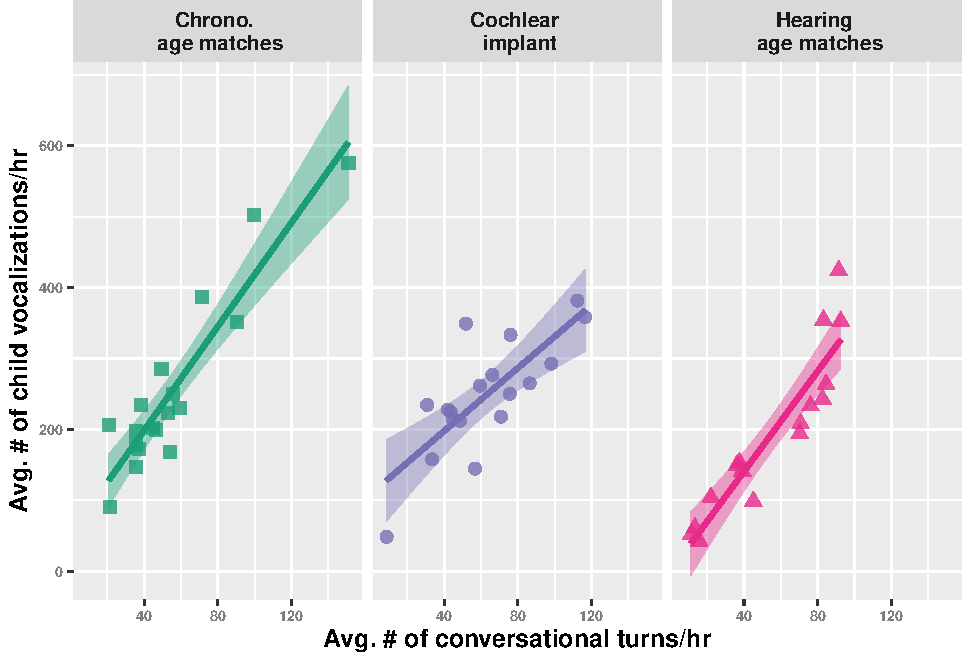
\includegraphics{everyday_CI_files/figure-latex/visualize input as turns predicting num vocalizations-1.pdf}

\begin{Shaded}
\begin{Highlighting}[]
\NormalTok{num\_vocs }\SpecialCharTok{\%\textgreater{}\%}
  \FunctionTok{mutate}\NormalTok{(}\AttributeTok{match=}\FunctionTok{factor}\NormalTok{(match, }\AttributeTok{levels=}\FunctionTok{c}\NormalTok{(}\StringTok{"chrono"}\NormalTok{, }\StringTok{"CI"}\NormalTok{, }\StringTok{"HA"}\NormalTok{))) }\SpecialCharTok{\%\textgreater{}\%}
  \FunctionTok{mutate}\NormalTok{(}\AttributeTok{match=}\FunctionTok{recode}\NormalTok{(match,}
                      \AttributeTok{chrono=}\StringTok{\textquotesingle{}Chrono. }\SpecialCharTok{\textbackslash{}n}\StringTok{ age matches\textquotesingle{}}\NormalTok{,}
                      \AttributeTok{CI=}\StringTok{\textquotesingle{}Cochlear }\SpecialCharTok{\textbackslash{}n}\StringTok{ implant\textquotesingle{}}\NormalTok{,}
                      \AttributeTok{HA=}\StringTok{\textquotesingle{}Hearing }\SpecialCharTok{\textbackslash{}n}\StringTok{ age matches\textquotesingle{}}\NormalTok{)) }\SpecialCharTok{\%\textgreater{}\%}
\FunctionTok{ggplot}\NormalTok{(., }\FunctionTok{aes}\NormalTok{(normed\_words, normed\_vocs)) }\SpecialCharTok{+}
  \FunctionTok{geom\_jitter}\NormalTok{(}\FunctionTok{aes}\NormalTok{(}\AttributeTok{color=}\NormalTok{match, }\AttributeTok{fill=}\NormalTok{match, }\AttributeTok{shape=}\NormalTok{match),}\AttributeTok{size=}\FloatTok{2.6}\NormalTok{,}\AttributeTok{alpha=}\NormalTok{.}\DecValTok{8}\NormalTok{,}\AttributeTok{width =}\NormalTok{ .}\DecValTok{3}\NormalTok{) }\SpecialCharTok{+}
  \FunctionTok{geom\_smooth}\NormalTok{(}\FunctionTok{aes}\NormalTok{(}\AttributeTok{fill=}\NormalTok{match, }\AttributeTok{color=}\NormalTok{match), }\AttributeTok{method =} \StringTok{"lm"}\NormalTok{,}\AttributeTok{size=}\FloatTok{1.2}\NormalTok{) }\SpecialCharTok{+} 
  \FunctionTok{facet\_grid}\NormalTok{(}\SpecialCharTok{\textasciitilde{}}\NormalTok{match) }\SpecialCharTok{+}
  \CommentTok{\#ylim(0, 600) +}
    \FunctionTok{scale\_color\_manual}\NormalTok{(}\AttributeTok{values=}\FunctionTok{c}\NormalTok{(}\StringTok{"\#1B9E77"}\NormalTok{, }\StringTok{"\#7570B3"}\NormalTok{, }\StringTok{"\#E7298A"}\NormalTok{))}\SpecialCharTok{+}
  \FunctionTok{scale\_fill\_manual}\NormalTok{(}\AttributeTok{values=}\FunctionTok{c}\NormalTok{(}\StringTok{"\#1B9E77"}\NormalTok{, }\StringTok{"\#7570B3"}\NormalTok{, }\StringTok{"\#E7298A"}\NormalTok{))}\SpecialCharTok{+}
  \FunctionTok{scale\_shape\_manual}\NormalTok{(}\AttributeTok{values=}\FunctionTok{c}\NormalTok{(}\DecValTok{15}\NormalTok{,}\DecValTok{16}\NormalTok{,}\DecValTok{17}\NormalTok{)) }\SpecialCharTok{+}
  \FunctionTok{xlab}\NormalTok{(}\StringTok{"Avg. \# of words from adults/hr"}\NormalTok{) }\SpecialCharTok{+}
  \FunctionTok{ylab}\NormalTok{(}\StringTok{"Avg. \# of child vocalizations/hr"}\NormalTok{) }\SpecialCharTok{+} 
    \FunctionTok{theme}\NormalTok{(}\AttributeTok{axis.title =} \FunctionTok{element\_text}\NormalTok{(}\AttributeTok{face =}\StringTok{"bold"}\NormalTok{, }\AttributeTok{size=}\DecValTok{12}\NormalTok{),}
        \AttributeTok{legend.position =} \StringTok{"none"}\NormalTok{, }
        \AttributeTok{axis.text =} \FunctionTok{element\_text}\NormalTok{(}\AttributeTok{face=}\StringTok{"bold"}\NormalTok{, }\AttributeTok{color=}\StringTok{\textquotesingle{}gray50\textquotesingle{}}\NormalTok{, }\AttributeTok{size=}\DecValTok{7}\NormalTok{),}
        \AttributeTok{strip.text=}\FunctionTok{element\_text}\NormalTok{(}\AttributeTok{face=}\StringTok{\textquotesingle{}bold\textquotesingle{}}\NormalTok{, }\AttributeTok{size=}\DecValTok{10}\NormalTok{))}
\end{Highlighting}
\end{Shaded}

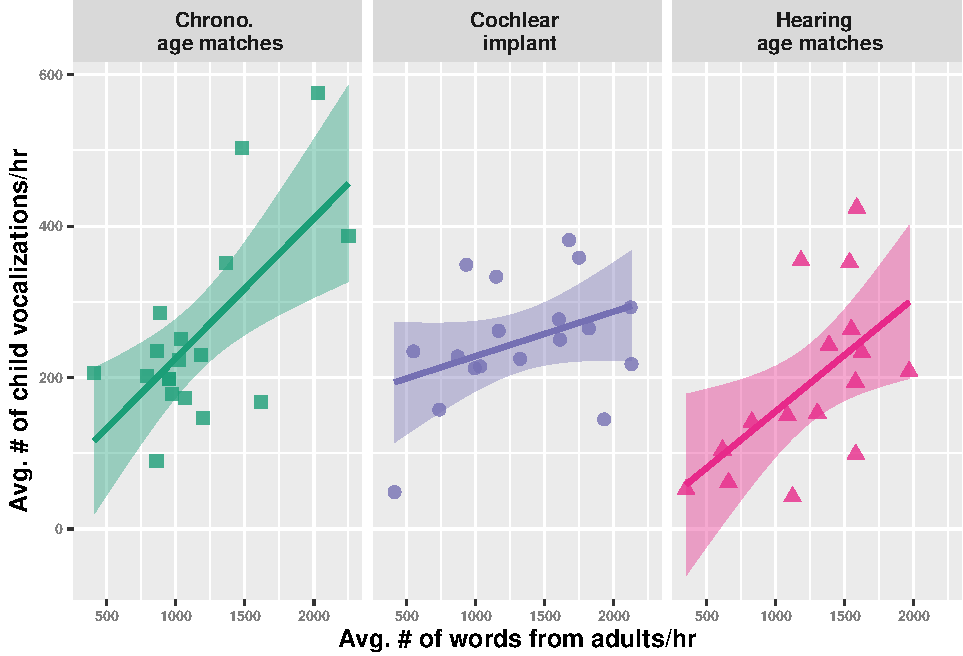
\includegraphics{everyday_CI_files/figure-latex/visualize input as words predicting num vocalizations-1.pdf}

\begin{Shaded}
\begin{Highlighting}[]
\NormalTok{num\_vocs }\OtherTok{\textless{}{-}}\NormalTok{ num\_vocs }\SpecialCharTok{\%\textgreater{}\%}
  \FunctionTok{mutate}\NormalTok{(}\AttributeTok{age\_mos\_centered =} \FunctionTok{center\_scale}\NormalTok{(age\_mos),}
         \AttributeTok{normed\_turns\_centered =} \FunctionTok{center\_scale}\NormalTok{(normed\_turns),}
         \AttributeTok{normed\_words\_centered =} \FunctionTok{center\_scale}\NormalTok{(normed\_words)) }

\CommentTok{\# which measure of input fits the outcome measure better?}
\NormalTok{num\_vocs}\SpecialCharTok{$}\NormalTok{match }\OtherTok{\textless{}{-}} \FunctionTok{relevel}\NormalTok{(}\FunctionTok{factor}\NormalTok{(num\_vocs}\SpecialCharTok{$}\NormalTok{match), }\AttributeTok{ref =} \StringTok{"CI"}\NormalTok{)}
\NormalTok{in\_out\_m0 }\OtherTok{\textless{}{-}} \FunctionTok{lm}\NormalTok{(normed\_vocs}\SpecialCharTok{\textasciitilde{}}\NormalTok{normed\_turns\_centered}\SpecialCharTok{+}\NormalTok{age\_mos\_centered, }\AttributeTok{data=}\NormalTok{num\_vocs)}
\NormalTok{in\_out\_m1 }\OtherTok{\textless{}{-}} \FunctionTok{lm}\NormalTok{(normed\_vocs}\SpecialCharTok{\textasciitilde{}}\NormalTok{normed\_words\_centered}\SpecialCharTok{+}\NormalTok{age\_mos\_centered, }\AttributeTok{data=}\NormalTok{num\_vocs)}
\CommentTok{\# turns results in a better model fit}
\FunctionTok{AIC}\NormalTok{(in\_out\_m0) }\CommentTok{\#560.5966}
\end{Highlighting}
\end{Shaded}

\begin{verbatim}
## [1] 560.5966
\end{verbatim}

\begin{Shaded}
\begin{Highlighting}[]
\FunctionTok{AIC}\NormalTok{(in\_out\_m1) }\CommentTok{\#611.2076}
\end{Highlighting}
\end{Shaded}

\begin{verbatim}
## [1] 611.2076
\end{verbatim}

\begin{Shaded}
\begin{Highlighting}[]
\CommentTok{\# match improves}
\NormalTok{in\_out\_m2 }\OtherTok{\textless{}{-}} \FunctionTok{lm}\NormalTok{(normed\_vocs}\SpecialCharTok{\textasciitilde{}}\NormalTok{match, }\AttributeTok{data=}\NormalTok{num\_vocs)}
\NormalTok{in\_out\_m3 }\OtherTok{\textless{}{-}} \FunctionTok{lm}\NormalTok{(normed\_vocs}\SpecialCharTok{\textasciitilde{}}\NormalTok{normed\_turns\_centered}\SpecialCharTok{+}\NormalTok{match, }\AttributeTok{data=}\NormalTok{num\_vocs)}
\FunctionTok{anova}\NormalTok{(in\_out\_m2,in\_out\_m3) }
\end{Highlighting}
\end{Shaded}

\begin{verbatim}
## Analysis of Variance Table
## 
## Model 1: normed_vocs ~ match
## Model 2: normed_vocs ~ normed_turns_centered + match
##   Res.Df    RSS Df Sum of Sq      F    Pr(>F)    
## 1     49 575123                                  
## 2     48 131913  1    443210 161.27 < 2.2e-16 ***
## ---
## Signif. codes:  0 '***' 0.001 '**' 0.01 '*' 0.05 '.' 0.1 ' ' 1
\end{verbatim}

\begin{Shaded}
\begin{Highlighting}[]
\CommentTok{\# interaction improves }
\NormalTok{in\_out\_m4 }\OtherTok{\textless{}{-}} \FunctionTok{lm}\NormalTok{(normed\_vocs}\SpecialCharTok{\textasciitilde{}}\NormalTok{normed\_turns\_centered}\SpecialCharTok{*}\NormalTok{match, }\AttributeTok{data=}\NormalTok{num\_vocs)}
\FunctionTok{anova}\NormalTok{(in\_out\_m3,in\_out\_m4)}
\end{Highlighting}
\end{Shaded}

\begin{verbatim}
## Analysis of Variance Table
## 
## Model 1: normed_vocs ~ normed_turns_centered + match
## Model 2: normed_vocs ~ normed_turns_centered * match
##   Res.Df    RSS Df Sum of Sq      F Pr(>F)  
## 1     48 131913                             
## 2     46 113563  2     18350 3.7165 0.0319 *
## ---
## Signif. codes:  0 '***' 0.001 '**' 0.01 '*' 0.05 '.' 0.1 ' ' 1
\end{verbatim}

\begin{Shaded}
\begin{Highlighting}[]
\CommentTok{\# repeated measures {-} not using}
\CommentTok{\#predict\_df \textless{}{-} num\_vocs \%\textgreater{}\%}
\CommentTok{\#  merge(., vocs, by=c(\textquotesingle{}child\_id\textquotesingle{}, \textquotesingle{}match\textquotesingle{}))}


\CommentTok{\#in\_out\_m2 \textless{}{-} lmer(log(childUttLen)\textasciitilde{}normed\_turns+match+(1|child\_id),data=predict\_df)}
\CommentTok{\#in\_out\_m3 \textless{}{-} lmer(log(childUttLen)\textasciitilde{}normed\_words*match+(1|child\_id),data=predict\_df)}
\CommentTok{\#in\_out\_m4 \textless{}{-} lmer(log(childUttLen)\textasciitilde{}normed\_turns*match+(1|child\_id),data=predict\_df)}
\end{Highlighting}
\end{Shaded}

\hypertarget{create-speech-measures-tables}{%
\section{Create speech measures tables}\label{create-speech-measures-tables}}

\hypertarget{standard-measures}{%
\subsection{Standard measures}\label{standard-measures}}

\begin{Shaded}
\begin{Highlighting}[]
\CommentTok{\# recording duration}
\NormalTok{rec\_dur\_tbl }\OtherTok{\textless{}{-}}\NormalTok{ its\_df }\SpecialCharTok{\%\textgreater{}\%}
  \FunctionTok{group\_by}\NormalTok{(match) }\SpecialCharTok{\%\textgreater{}\%}
  \FunctionTok{summarize}\NormalTok{(}\AttributeTok{recording\_duration =} \FunctionTok{mean}\NormalTok{(total\_hrs),}
            \AttributeTok{recording\_duration\_sd =} \FunctionTok{sd}\NormalTok{(total\_hrs),}
            \AttributeTok{recording\_duration\_min =} \FunctionTok{min}\NormalTok{(total\_hrs),}
            \AttributeTok{recording\_duration\_max =} \FunctionTok{max}\NormalTok{(total\_hrs)) }\SpecialCharTok{\%\textgreater{}\%}
  \FunctionTok{mutate\_if}\NormalTok{(is.numeric, round, }\DecValTok{2}\NormalTok{) }\SpecialCharTok{\%\textgreater{}\%}
  \FunctionTok{mutate}\NormalTok{(}\AttributeTok{recording\_stats =} \FunctionTok{paste0}\NormalTok{(recording\_duration,}\StringTok{"("}\NormalTok{,recording\_duration\_sd,}\StringTok{")"}\NormalTok{,}\StringTok{","}\NormalTok{,recording\_duration\_min,}\StringTok{"{-}"}\NormalTok{,recording\_duration\_max)) }\SpecialCharTok{\%\textgreater{}\%}
  \FunctionTok{select}\NormalTok{(match, recording\_stats) }\SpecialCharTok{\%\textgreater{}\%}
  \FunctionTok{spread}\NormalTok{(match, recording\_stats) }\SpecialCharTok{\%\textgreater{}\%}
  \FunctionTok{rownames\_to\_column}\NormalTok{(.,}\AttributeTok{var =} \StringTok{\textquotesingle{}measure\textquotesingle{}}\NormalTok{)}

\CommentTok{\# Input}
\NormalTok{speech\_quantity\_tbl}
\end{Highlighting}
\end{Shaded}

\begin{verbatim}
## # A tibble: 3 x 4
##   measure        chrono                         CI                         HA   
##   <chr>          <chr>                          <chr>                      <chr>
## 1 intensity      68.12(5.98),47.1-84.22         68.82(5.87),45.46-84.2     68.7~
## 2 num_words_hr   1162.83(448.41),408.96-2250.39 1321.66(528.56),411.36-21~ 1246~
## 3 mins_speech_hr 291.29(111.26),112.59-545.81   327(125.54),100.7-514.19   314.~
\end{verbatim}

\begin{Shaded}
\begin{Highlighting}[]
\NormalTok{speech\_consis\_tbl}
\end{Highlighting}
\end{Shaded}

\begin{verbatim}
## # A tibble: 1 x 4
##   measure chrono               CI                   HA                  
##   <chr>   <chr>                <chr>                <chr>               
## 1 1       0.53(0.12),0.35-0.78 0.59(0.12),0.25-0.73 0.53(0.11),0.31-0.66
\end{verbatim}

\begin{Shaded}
\begin{Highlighting}[]
\CommentTok{\# Output}
\NormalTok{voc\_tbl}
\end{Highlighting}
\end{Shaded}

\begin{verbatim}
## # A tibble: 3 x 4
##   measure     chrono                      CI                         HA         
##   <chr>       <chr>                       <chr>                      <chr>      
## 1 intensity   76.78(4.39),47.51-84.77     76.95(4.35),43.16-85.79    77.15(4.95~
## 2 num_vocs_hr 308.03(142.81),90.12-575.81 271.75(69.23),48.75-381.62 254.5(108.~
## 3 voc_dur     1004.46(662.3),80-10940     937.93(569.76),80-13270    966.59(627~
\end{verbatim}

\begin{Shaded}
\begin{Highlighting}[]
\NormalTok{voc\_consis\_tbl}
\end{Highlighting}
\end{Shaded}

\begin{verbatim}
## # A tibble: 1 x 4
##   measure chrono               CI                   HA                  
##   <chr>   <chr>                <chr>                <chr>               
## 1 1       0.55(0.15),0.34-0.84 0.58(0.13),0.17-0.72 0.49(0.14),0.22-0.69
\end{verbatim}

\begin{Shaded}
\begin{Highlighting}[]
\CommentTok{\# Interaction}
\NormalTok{convo\_consis\_tbl}
\end{Highlighting}
\end{Shaded}

\begin{verbatim}
## # A tibble: 1 x 4
##   measure chrono               CI                   HA                  
##   <chr>   <chr>                <chr>                <chr>               
## 1 1       0.58(0.14),0.38-0.84 0.64(0.13),0.22-0.77 0.56(0.12),0.36-0.74
\end{verbatim}

\begin{Shaded}
\begin{Highlighting}[]
\NormalTok{turn\_quantity\_tbl}
\end{Highlighting}
\end{Shaded}

\begin{verbatim}
## # A tibble: 1 x 4
##   measure chrono                    CI                      HA                  
##   <chr>   <chr>                     <chr>                   <chr>               
## 1 1       61.71(32.78),20.69-150.94 68.17(26.47),8.5-116.75 65.13(25.47),11.12-~
\end{verbatim}

\begin{Shaded}
\begin{Highlighting}[]
\NormalTok{measure\_tbl }\OtherTok{\textless{}{-}}\NormalTok{ rec\_dur\_tbl }\SpecialCharTok{\%\textgreater{}\%}
  \FunctionTok{rbind}\NormalTok{(., speech\_quantity\_tbl) }\SpecialCharTok{\%\textgreater{}\%}
  \FunctionTok{rbind}\NormalTok{(., speech\_consis\_tbl) }\SpecialCharTok{\%\textgreater{}\%}
  \FunctionTok{rbind}\NormalTok{(., voc\_tbl) }\SpecialCharTok{\%\textgreater{}\%}
  \FunctionTok{rbind}\NormalTok{(., voc\_consis\_tbl) }\SpecialCharTok{\%\textgreater{}\%}
  \FunctionTok{rbind}\NormalTok{(., turn\_quantity\_tbl) }\SpecialCharTok{\%\textgreater{}\%}
  \FunctionTok{rbind}\NormalTok{(., convo\_consis\_tbl) }
  
\NormalTok{meas\_mat }\OtherTok{\textless{}{-}}\NormalTok{ measure\_tbl }\SpecialCharTok{\%\textgreater{}\%} \FunctionTok{select}\NormalTok{(}\SpecialCharTok{{-}}\NormalTok{measure) }\SpecialCharTok{\%\textgreater{}\%} \FunctionTok{as.matrix}\NormalTok{(.)}

\FunctionTok{row.names}\NormalTok{(meas\_mat) }\OtherTok{\textless{}{-}} \FunctionTok{c}\NormalTok{(}\StringTok{"Recording duration (hrs.)"}\NormalTok{,}
                           \StringTok{"Adult speech intensity (dB)"}\NormalTok{,}
                           \StringTok{"Adult speech/hr (words)"}\NormalTok{,}
                           \StringTok{"Adult speech/hr (s)"}\NormalTok{,}
                           \StringTok{"Adult word consistency"}\NormalTok{,}
                           \StringTok{"Voc. intensity (dB)"}\NormalTok{,}
                           \StringTok{"Child voc. quantity"}\NormalTok{,}
                           \StringTok{"Voc. duration (ms)"}\NormalTok{,}
                           \StringTok{"Child voc. consistency"}\NormalTok{,}
                           \CommentTok{\#"Input:output", \# maybe include this?}
                           \CommentTok{\#"\% contingent vocs.",}
                           \StringTok{"Convo. turn quantity"}\NormalTok{,}
                           \StringTok{"Convo turn consistency"}\NormalTok{)}


\FunctionTok{kable}\NormalTok{(meas\_mat,}
             \AttributeTok{caption=} \StringTok{"Measures of the naturalistic speech environment, by hearing group"}\NormalTok{,}
             \AttributeTok{col.names =} \FunctionTok{c}\NormalTok{(}\StringTok{"Chrono. age matches"}\NormalTok{, }
                           \StringTok{"CI"}\NormalTok{, }
                           \StringTok{"Hearing age matches"}\NormalTok{),}
      \AttributeTok{escape=}\ConstantTok{FALSE}\NormalTok{) }\SpecialCharTok{\%\textgreater{}\%} 
  \FunctionTok{kable\_styling}\NormalTok{(.) }\SpecialCharTok{\%\textgreater{}\%}
  \FunctionTok{pack\_rows}\NormalTok{(., }\StringTok{"Recording"}\NormalTok{, }\DecValTok{1}\NormalTok{, }\DecValTok{1}\NormalTok{) }\SpecialCharTok{\%\textgreater{}\%}
  \FunctionTok{pack\_rows}\NormalTok{(., }\StringTok{"Input"}\NormalTok{, }\DecValTok{2}\NormalTok{,}\DecValTok{5}\NormalTok{) }\SpecialCharTok{\%\textgreater{}\%}
  \FunctionTok{pack\_rows}\NormalTok{(., }\StringTok{"Output"}\NormalTok{, }\DecValTok{6}\NormalTok{,}\DecValTok{9}\NormalTok{) }\SpecialCharTok{\%\textgreater{}\%}
  \FunctionTok{pack\_rows}\NormalTok{(., }\StringTok{"Interaction"}\NormalTok{, }\DecValTok{10}\NormalTok{,}\DecValTok{11}\NormalTok{)}
\end{Highlighting}
\end{Shaded}

\begin{table}

\caption{(\#tab:create standard measures table)Measures of the naturalistic speech environment, by hearing group}
\centering
\begin{tabular}[t]{l|l|l|l}
\hline
  & Chrono. age matches & CI & Hearing age matches\\
\hline
\multicolumn{4}{l}{\textbf{Recording}}\\
\hline
\hspace{1em}Recording duration (hrs.) & 15.82(0.75),12.83-16 & 16(0),16-16 & 16(0),16-16\\
\hline
\multicolumn{4}{l}{\textbf{Input}}\\
\hline
\hspace{1em}Adult speech intensity (dB) & 68.12(5.98),47.1-84.22 & 68.82(5.87),45.46-84.2 & 68.73(6.19),44.92-88.4\\
\hline
\hspace{1em}Adult speech/hr (words) & 1162.83(448.41),408.96-2250.39 & 1321.66(528.56),411.36-2127.7 & 1246.53(444.48),350.59-1966.41\\
\hline
\hspace{1em}Adult speech/hr (s) & 291.29(111.26),112.59-545.81 & 327(125.54),100.7-514.19 & 314.5(104.37),107.19-473.13\\
\hline
\hspace{1em}Adult word consistency & 0.53(0.12),0.35-0.78 & 0.59(0.12),0.25-0.73 & 0.53(0.11),0.31-0.66\\
\hline
\multicolumn{4}{l}{\textbf{Output}}\\
\hline
\hspace{1em}Voc. intensity (dB) & 76.78(4.39),47.51-84.77 & 76.95(4.35),43.16-85.79 & 77.15(4.95),44.79-90.31\\
\hline
\hspace{1em}Child voc. quantity & 308.03(142.81),90.12-575.81 & 271.75(69.23),48.75-381.62 & 254.5(108.83),42.5-424\\
\hline
\hspace{1em}Voc. duration (ms) & 1004.46(662.3),80-10940 & 937.93(569.76),80-13270 & 966.59(627.6),80-19730\\
\hline
\hspace{1em}Child voc. consistency & 0.55(0.15),0.34-0.84 & 0.58(0.13),0.17-0.72 & 0.49(0.14),0.22-0.69\\
\hline
\multicolumn{4}{l}{\textbf{Interaction}}\\
\hline
\hspace{1em}Convo. turn quantity & 61.71(32.78),20.69-150.94 & 68.17(26.47),8.5-116.75 & 65.13(25.47),11.12-92.62\\
\hline
\hspace{1em}Convo turn consistency & 0.58(0.14),0.38-0.84 & 0.64(0.13),0.22-0.77 & 0.56(0.12),0.36-0.74\\
\hline
\end{tabular}
\end{table}

\hypertarget{growth-in-measures-table}{%
\subsection{Growth in measures table}\label{growth-in-measures-table}}

\begin{Shaded}
\begin{Highlighting}[]
\CommentTok{\# we create a separate table here because comparing four "matches" (to include growth by hearing age)}
\NormalTok{growth\_tbl }\OtherTok{\textless{}{-}}\NormalTok{ input\_growth\_tbl  }\SpecialCharTok{\%\textgreater{}\%}
  \FunctionTok{rbind}\NormalTok{(., voc\_growth\_tbl) }\SpecialCharTok{\%\textgreater{}\%}
  \FunctionTok{rbind}\NormalTok{(., voc\_dur\_growth\_tbl) }\SpecialCharTok{\%\textgreater{}\%}
  \FunctionTok{rbind}\NormalTok{(., ctc\_growth\_tbl) }\SpecialCharTok{\%\textgreater{}\%}
  \FunctionTok{select}\NormalTok{(measure, chrono, CI, CI\_by\_hearing\_age, HA)}


\FunctionTok{kable}\NormalTok{(growth\_tbl, }\AttributeTok{booktabs=}\NormalTok{T, }
              \AttributeTok{caption=} \StringTok{"Growth in measures of the naturalistic speech environment, by hearing group"}\NormalTok{,}
              \AttributeTok{col.names =} \FunctionTok{c}\NormalTok{(}\StringTok{" "}\NormalTok{, }
                            \StringTok{"Chrono. age matches"}\NormalTok{, }
                           \StringTok{"CI by chrono. age"}\NormalTok{, }
                           \StringTok{"CI by hearing age"}\NormalTok{, }
                           \StringTok{"Hearing age matches"}\NormalTok{)) }\SpecialCharTok{\%\textgreater{}\%}
  \FunctionTok{kable\_styling}\NormalTok{() }\SpecialCharTok{\%\textgreater{}\%}
  \FunctionTok{kable\_styling}\NormalTok{(}\AttributeTok{latex\_options =} \StringTok{"hold\_position"}\NormalTok{)}
\end{Highlighting}
\end{Shaded}

\begin{table}[!h]

\caption{(\#tab:create growth table)Growth in measures of the naturalistic speech environment, by hearing group}
\centering
\begin{tabular}[t]{lllll}
\toprule
  & Chrono. age matches & CI by chrono. age & CI by hearing age & Hearing age matches\\
\midrule
Adult word growth & B=14.1,p=0.17,r=0.34 & B=1.03,p=0.94,r=0.02 & B=-2.03,p=0.86,r=-0.05 & B=22.03,p=0.01,r=0.63\\
Child voc. quantity growth & B=3.98,p=0.16,r=0.34 & B=2.71,p=0.19,r=0.33 & B=1.06,p=0.53,r=0.17 & B=8.03,p=0,r=0.89\\
Child voc. duration growth (ms) & B=564.77,p=0.79,r=0.07 & B=3168.23,p=0.05,r=0.47 & B=1850.89,p=0.18,r=0.35 & B=6584.89,p=0,r=0.73\\
Convo. turn growth & B=0.83,p=0.25,r=0.29 & B=0.01,p=0.99,r=0 & B=-0.33,p=0.56,r=-0.16 & B=2.18,p=0,r=0.93\\
\bottomrule
\end{tabular}
\end{table}

\begin{Shaded}
\begin{Highlighting}[]
\CommentTok{\# note that in the ICPhS paper I reported the p{-}value for CI hearing age that included the two kids}
\CommentTok{\# with HA \textless{} 12}
\end{Highlighting}
\end{Shaded}


\end{document}
